\documentclass[a4paper,12pt,titlepage]{report}  

% Pacchetti per la lingua e la grafica
\usepackage[utf8]{inputenc}            % Codifica dei caratteri in UTF-8
\usepackage[T1]{fontenc}               % Codifica dei font in T1
\usepackage[italian]{babel}            % Imposta l'italiano come lingua principale
\usepackage{graphicx}                  % Per inserire immagini
\usepackage{caption}                   % Per personalizzare le didascalie delle immagini
\usepackage{subcaption}                % Per didascalie delle sotto-figure
\usepackage{amsmath, amssymb, amsthm, mathrsfs}  % Pacchetti per la matematica avanzata
\usepackage{hyperref}                  % Per i link interni ed esterni
\usepackage{geometry}                  % Per personalizzare i margini della pagina
\geometry{a4paper, margin=2.5cm}       % Margini personalizzati 
\usepackage{setspace}                  % Per gestire l'interlinea
\usepackage{fancyhdr}                  % Per personalizzare intestazioni e piè di pagina
\usepackage{pdfpages}                  % Per inserire pagine PDF nel documento
\usepackage{frontespizio}
\usepackage{tikz}
\usepackage{float}
\usepackage[font=small,labelfont=bf,width=0.8\textwidth]{caption}
\usepackage[autostyle,italian=guillemets]{csquotes}
\usepackage[backend=biber]{biblatex}
\addbibresource{bibliografia.bib}

% Definizioni di teoremi, lemmi, corollari, ecc.
\newtheorem{theorem}{Teorema}[chapter]
\newtheorem{lemma}[theorem]{Lemma}
\newtheorem{corollary}[theorem]{Corollario}
\newtheorem{definition}{Definizione}[chapter]

% Impostazioni di base per l'intestazione e il piè di pagina
\pagestyle{fancy}
\fancyhead{}
\fancyfoot{}
\fancyhead[L]{\leftmark}               % Intestazione sinistra con il titolo del capitolo
\fancyfoot[C]{\thepage}                % Piè di pagina centrale con il numero di pagina

% Link colorati
\hypersetup{
	colorlinks=true,                   % false: link con riquadri; true: link colorati
	linkcolor=black,                    % Colore dei link interni
	citecolor=black,                   % Colore delle citazioni
	filecolor=magenta,                 % Colore dei file allegati
	urlcolor=cyan                      % Colore degli URL
}

% Impostazioni per l'interlinea
\onehalfspacing                       % Interlinea di 1.5

\begin{document}
	
	\begin{frontespizio}
		\Universita{Padova}
		\Logo[2.5cm]{Logo_Unipd}
		\Dipartimento{Matematica\\''Tullio Levi-Civita''}
		\Corso[Laurea]{Matematica}
		\Annoaccademico{2023--2024}
		\Titoletto{\large Tesi di Laurea}
		\Titolo{Il Teorema dei Quattro Colori:\\Storia e Dimostrazioni}
		\Candidato[1220520]{Riccardo Pilan}
		\Relatore{Prof. Manuel Francesco Aprile}
	\end{frontespizio}   
	                         
	\newpage
	\thispagestyle{empty}
	\null
	\newpage
	\setcounter{page}{1} % Ripristina il numero di pagina a 1
	
	\tableofcontents
	 
	\newpage
	\null                       
	
	\chapter{Introduzione}                
	
	\section{Premessa}
	Il Teorema dei Quattro Colori rappresenta forse uno dei risultati più interessanti, rivoluzionari e controversi della storia della matematica.
	\\L’enunciato del Teorema è in realtà piuttosto semplice: data una mappa geografica, o, in generale, una superficie piana suddivisa in regioni connesse, è sempre possibile colorarne le regioni utilizzando al massimo quattro colori diversi, ponendo come regola che due territori confinanti non condividano lo stesso colore.
	\\Nonostante la semplicità della sua formulazione, il Teorema ha impegnato per oltre un secolo le menti di alcuni tra i più illustri matematici del diciannovesimo e ventesimo secolo, tra dimostrazioni rivelatesi errate, vari tentativi di approccio al problema utilizzando tecniche differenti e lo sviluppo di una vera e propria nuova branca della matematica, la Teoria dei grafi, fino a giungere a una delle dimostrazioni più controverse e divisive di sempre all’interno della comunità matematica.
	
	\section{Breve storia del Teorema}
	La prima formulazione del Teorema risale al 1852 ed è da attribuire a Francis Guthrie, ma è grazie a De Morgan e Cayley che la comunità matematica ne viene a conoscenza. 
	\\I primi contributi importanti nella ricerca di una soluzione sono datati 1879 e 1880 e consistono in due dimostrazioni, rivelatesi entrambe errate, da parte rispettivamente di Kempe e Tait, confutate da Heawood nel 1890 e da Petersen nel 1891, ma contenenti una serie di tecniche e risultati di grande rilevanza per gli sviluppi successivi.
	\\Per quasi un secolo, nonostante le formulazioni alternative, lo sviluppo della Teoria dei grafi, i diversi approcci tentati e le nuove tecniche utilizzate, sono pochi i passi compiuti verso una vera e propria dimostrazione della Congettura; fino a giungere al 1976, quando Appel e Haken pubblicano una dimostrazione completamente diversa da qualunque risultato ottenuto precedentemente in ambito matematico, a causa di un uso estensivo del computer per l’analisi, caso per caso, di una serie di numerose configurazioni.
	\\La dimostrazione scatena grandi controversie e divide la comunità matematica per via dell’utilizzo della cosiddetta “forza bruta” e quindi per la sua scarsa eleganza, ma soprattutto per l’impossibilità di verificare manualmente che il computer non abbia commesso errori e che l’algoritmo utilizzato da esso funzioni correttamente.
	\\Tuttavia, il metodo utilizzato per ottenere il risultato è rivoluzionario e sancisce l’inizio dell’era delle dimostrazioni assistite da computer, portando a una grande svolta nel mondo della matematica.
	\\Inoltre, nel 1996, 4 matematici, a cui ci riferiremo come Robertson et al., pubblicano una nuova dimostrazione che risulta essere una versione più efficiente e meno controversa di quella di Appel e Haken, sarà infatti quella che verrà trattata in questa tesi.
	
	\section{Scopo e struttura della tesi}
	Questa tesi ha un duplice scopo, si propone di analizzare il Teorema dei Quattro Colori da due punti di vista ugualmente significativi: da un lato verrà approfondita la parte storica del Teorema, con particolare interesse verso le sue origini, le dimostrazioni tentate, lo sviluppo delle tecniche che hanno contribuito alla dimostrazione definitiva e le figure chiave coinvolte nella diffusione e nello studio del problema; dall’altro lato verrà esaminato il contenuto matematico del Teorema, nello specifico l’utilizzo della Teoria dei grafi per affrontare la Congettura, la serie di teoremi e risultati che hanno preceduto e ispirato Appel e Haken (e Robertson et al.), le tecniche da loro utilizzate nella dimostrazione finale e infine le generalizzazioni del Teorema e gli sviluppi più recenti.
	\\In particolare, in seguito a questo primo capitolo introduttivo, il capitolo 2 ripercorrerà in modo più dettagliato la storia del Teorema, dalle sue origini alla sua dimostrazione finale.
	\\Il capitolo 3 sarà dedicato alle basi matematiche necessarie per la comprensione della dimostrazione del Teorema: definizioni fondamentali di Teoria dei grafi, passaggio da mappe a grafi duali e riformulazione del Teorema in termini di grafi.
	\\Il capitolo 4 conterrà invece una formulazione matematica dettagliata della dimostrazione errata di Kempe, dell'errore contenuto in essa e della dimostrazione del Teorema dei Cinque Colori formulata da Heawood.
	\\Il capitolo 5 sarà quello dedicato alla vera e propria dimostrazione del Teorema dei Quattro Colori, in questo caso specifico la dimostrazione successiva pubblicata da Robertson et al. e non quella di Appel e Haken.
	\\Infine, il capitolo 6 sarà dedicato alle conclusioni, tra accenni a generalizzazioni del Teorema e problemi ancora aperti correlati ad esso, possibili evoluzioni della ricerca in questo campo e considerazioni finali sull’importanza e l’impatto rivestito dal Teorema nella storia della matematica.
	
	\chapter[Storia del Teorema]{Storia del Teorema dei Quattro Colori}
	In questo capitolo ripercorriamo la storia del Teorema dei Quattro Colori, facendo riferimento principalmente a {\bfseries \cite{Saaty}} e {\bfseries \cite{Turner}}.
	\section[Origine del Teorema]{Origine del Teorema (1852-1878)}
	Il Teorema viene enunciato per la prima volta sotto forma di Congettura dei Quattro Colori nel 1852, quando il giovane matematico britannico Francis Guthrie, intento a colorare una cartina delle contee d’Inghilterra, si rende conto che è possibile utilizzare soltanto quattro colori diversi per completarla, con la restrizione che due territori limitrofi presentino una colorazione differente.
	\\Guthrie, dopo una serie di tentativi, ipotizza che sia possibile fare lo stesso per qualunque cartina geografica ed espone la sua congettura al fratello Frederick, studente presso lo University College di Londra del professor Augustus De Morgan, il quale, venuto a conoscenza del problema, lo porta all’attenzione dei suoi studenti e della comunità matematica, dando credito a Guthrie.
	\\Non si verificano ulteriori sviluppi fino al 1878, quando Arthur Cayley si riferisce alla Congettura in uno scritto presentato presso la London Mathematical Society, affrontando un primo studio del problema e chiedendo ai propri colleghi se sia stata trovata una dimostrazione, scatenando definitivamente l’interesse dei matematici nella ricerca di una soluzione.
	\vspace{0.5cm}
	
	A questo punto è opportuno definire formalmente cosa si intenda per mappa, quando due regioni si considerano confinanti ed enunciare la Congettura nella sua forma originale.
    \newline 
	\theoremstyle{definition}
	\newtheorem{dfn}{Definizione}[chapter]
	\begin{dfn} 
		\medspace
		\begin{enumerate}
		\item Si dice {\bfseries mappa planare} una partizione del piano in sottoinsiemi disgiunti e connessi, che chiameremo \emph{regioni}, legate da rapporti di adiacenza.
		\item Due regioni si dicono {\bfseries adiacenti} o {\bfseries confinanti} se condividono un segmento di confine. 
        \end{enumerate}
        \emph{Note}: 
        \begin{enumerate}
        	\item Tutte le regioni devono essere connesse, perciò non è ammesso il caso di exclavi territoriali.
        	\item Date due regioni $R_{1}$ ed $R_{2}$, se Frontiera($R_{1}$) $\bigcap$ Frontiera($R_{2}$) $\ne$ 0, le due regioni non sono necessariamente confinanti, poiché le due frontiere potrebbero condividere un unico punto, mentre nella definizione che abbiamo fornito è richiesto che condividano un segmento.
        \end{enumerate}
	\end{dfn}
	\vspace{0.5cm}
	\newtheorem*{auxnamedthm*}{\nameofthethm}
	\newenvironment{namedthm*}[1]{
	\newcommand{\nameofthethm}{#1}
	\begin{auxnamedthm*}}
	{\end{auxnamedthm*}}
	\begin{namedthm*}{Congettura dei Quattro Colori (Guthrie, 1852)}
		Ogni mappa planare ammette una colorazione delle proprie regioni che prevede l'utilizzo di un massimo di 4 colori diversi, con la condizione che due regioni confinanti non abbiano lo stesso colore.
	\end{namedthm*}
	\begin{figure}[h]
		\centering
		\begin{tikzpicture}
			\node[anchor=south west, inner sep=0] (image) at (0,0) 
			{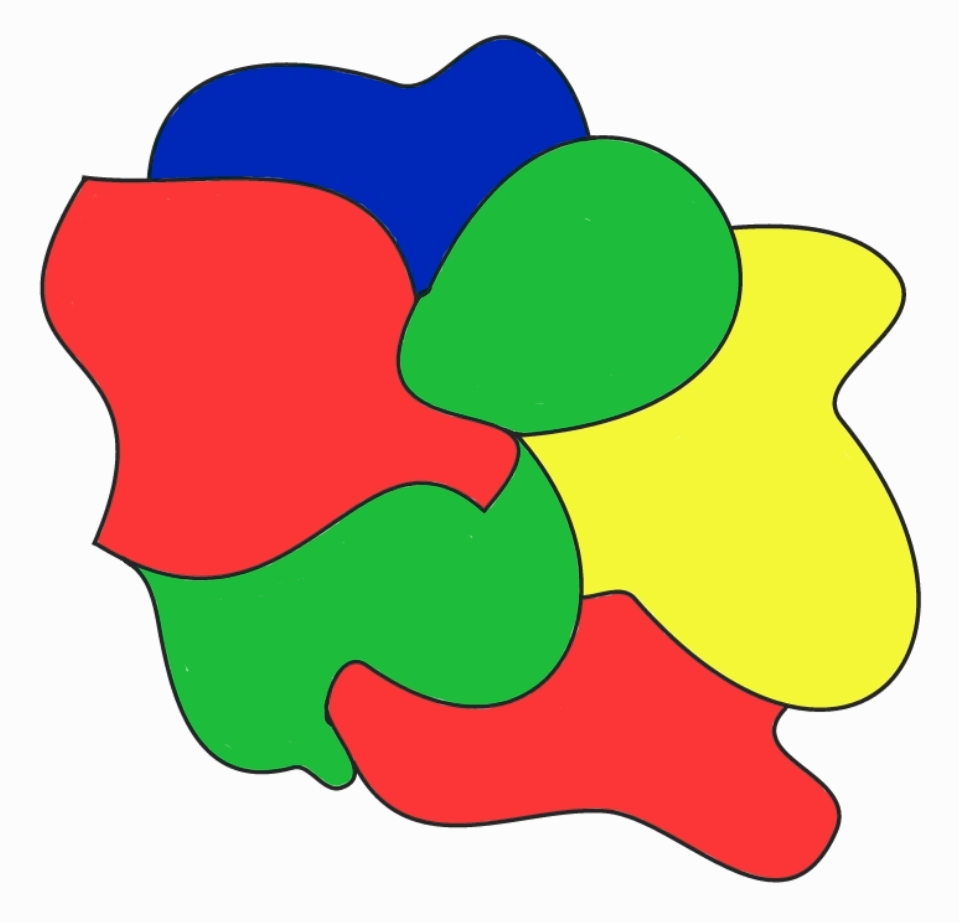
\includegraphics[width=0.5\textwidth]{Mappa.jpg}}; 
			\begin{scope}[x={(image.south east)},y={(image.north west)}]
				\node[text=white] at (0.4, 0.83) {$R_1$};
				\node at (0.78, 0.45) {$R_5$};
				\node at (0.6, 0.7) {$R_3$};
				\node at (0.38, 0.35) {$R_4$};
				\node at (0.6, 0.2) {$R_6$};
				\node at (0.25,0.6) {$R_2$};
			\end{scope}
		\end{tikzpicture}
		\caption{Esempio di mappa planare con 6 regioni colorata utilizzando 4 colori. Le regioni $R_3$ ed $R_4$ non sono confinanti, come spiegato nella Nota 2, quindi possono avere la stessa colorazione.}
		\label{fig:mappa}
	\end{figure}
	\vspace{0.5cm}
	
	Quella appena enunciata è la formulazione della Congettura nella sua forma originale, con riferimento a mappe planari e senza accenni alla Teoria dei grafi.
	\\Per molti anni i matematici che si sono dedicati allo studio della Congettura si sono serviti di mappe, ma la definizione di grafo duale di una mappa planare (che verrà data nel capitolo 3) ha costituito un punto di svolta fondamentale nella ricerca della dimostrazione.
	
	\section[Le dimostrazioni errate]{Le dimostrazioni errate di Kempe e Tait (1879-1891)}
	Nel 1879, l’anno successivo allo scritto di Cayley, Alfred Bray Kempe annuncia di aver trovato una dimostrazione alla Congettura dei Quattro Colori {\bfseries \cite{Kempe}}.
	\\La dimostrazione viene accolta con entusiasmo e clamore dalla comunità matematica e a Kempe vengono riconosciuti grandi meriti, tra cui l'ammissione alla Royal Society nel 1881. \\Tuttavia 11 anni dopo, nel 1890, Percy John Heawood scopre un errore nel suddetto risultato, in quanto la dimostrazione di Kempe, che fornisce anche un algoritmo per la colorazione delle mappe, risulta non essere valida in alcuni casi particolari, trascurati dallo stesso Kempe.
	\\Heawood, tuttavia, sfrutta le tecniche utilizzate per dimostrare un risultato più debole, il Teorema dei Cinque Colori, in particolare servendosi delle cosiddette \emph{catene di Kempe (Kempe chains)}, ideate dallo stesso Kempe.
	
	Definiamo allora il Teorema dei Cinque Colori:
	\begin{namedthm*}{Teorema dei Cinque Colori (Heawood, 1890)}
		Ogni mappa planare ammette una colorazione delle proprie regioni che prevede l'utilizzo di un massimo di 5 colori diversi, con la condizione che due regioni confinanti non abbiano lo stesso colore.
	\end{namedthm*}
	Il Teorema dei Cinque Colori verrà ripreso nel dettaglio e dimostrato nel capitolo 4.
	\\Ad appena un anno di distanza da quella di Kempe, nel 1880, anche Peter Guthrie Tait presenta una dimostrazione alla Congettura, indipendente dalla prima, ma basata su un’assunzione errata, come dimostrato da Julius Petersen nel 1891. 
	\\Anche in questo caso però la dimostrazione fornisce a Petersen gli strumenti per riformulare la Congettura dei Quattro Colori in due versioni differenti da quella originale, fornendo così spunti ad approcci differenti e possibili dimostrazioni alternative.
	
	\section[Sviluppi successivi]{Sviluppi successivi (1892-1975)}
	 In seguito alle due dimostrazioni fallite, la ricerca di una dimostrazione diretta del Teorema viene abbandonata e gli sforzi dei matematici si concentrano sulla ricerca di una dimostrazione per contraddizione. 
	 \\La dimostrazione si sviluppa nel modo seguente: si suppone per assurdo che la Congettura dei Quattro Colori sia errata, di conseguenza deve esistere un controesempio ad essa, e in particolare si considera il minimo controesempio, ovvero la mappa planare con il minor numero possibile di regioni che sia colorabile utilizzando 5 colori, ma non 4. Si individuano poi una serie di caratteristiche del minimo controesempio che portano a una contraddizione, dimostrando così che non può esistere un minimo controesempio alla Congettura (e di conseguenza nessun altro controesempio), provando così anche la validità della Congettura dei Quattro Colori.
	 \\Un gran numero di matematici si interessa al problema e si susseguono risultati parziali, generalizzazioni e nuove caratterizzazioni della Congettura dei Quattro Colori.
	 \\Nel 1898 il già citato Heawood trasforma la Congettura in una forma algebrica equivalente; similmente nel 1912 Oswald Veblen la riscrive in termini di geometria proiettiva.
	 \\Tra il 1912 e il 1913 George David Birkhoff introduce per la prima volta due concetti di grandissima rilevanza: il \emph{polinomio cromatico}, che esprime il numero di colorazioni di una mappa (o grafo) in funzione del numero di colori disponibili, con successive applicazioni legate non soltanto al Teorema dei Quattro Colori, ma anche alla Teoria dei grafi e persino alla Fisica statistica; e la \emph{riducibilità delle mappe} {\bfseries \cite{Birkhoff}}, idea fondamentale per giungere alla soluzione definitiva del problema, utilizzata da Appel e Haken nella dimostrazione finale.
	 % definizione/esempio di polinomio cromatico e riducibilità?
	 \\Nel 1931 Hassler Whitney, nella sua tesi di dottorato, sotto la supervisione dello stesso Birkhoff, definisce il \emph{grafo duale} di una mappa planare; individua in questo modo la relazione che lega mappe e grafi, contribuendo in modo determinante allo sviluppo della Teoria dei Grafi anche come strumento per affrontare la Congettura dei Quattro Colori, ormai irrisolta da quasi 80 anni.
	 \\Tra il 1922 e il 1940 i matematici Philip Franklin, Alfred Errera, Clarence Reynolds e C. N. Winn pubblicano una serie di risultati riguardanti le caratteristiche di un minimo controesempio al Teorema dei Quattro Colori, dimostrando dapprima che una tale mappa deve necessariamente essere costituita da almeno 26 regioni e successivamente portando il limite inferiore a 36 regioni, di cui almeno 15 pentagoni.
	 \\Al 1941 risale un importante risultato riguardante il numero cromatico di un grafo, ossia il numero minimo di colori necessari per colorarlo, il Teorema di Brooks, che deve il nome al matematico inglese Rowland Leonard Brooks e fornisce una relazione tra numero cromatico e grado di un grafo.
	 \\È datata invece 1943 la \emph{Congettura di Hadwiger}, ideata da Hugo Hadwiger, una generalizzazione del Teorema dei Quattro Colori tuttora irrisolta, uno dei più importanti problemi aperti nella Teoria dei grafi, che riprenderemo anche nella parte finale della tesi.
	 \\Nel 1969 il tedesco Heinrich Heesch pubblica uno scritto {\bfseries \cite{Heesch}} nel quale elabora per la prima volta un metodo per assegnare una carica ai vertici di un grafo e descrive il processo di \emph{scarica (discharging)}, un concetto che risulterà essenziale nella dimostrazione di Appel e Haken del 1976, tuttavia Heesch non riesce a giungere a una dimostrazione definitiva della Congettura perché non dispone di computer dotati di potenza di calcolo sufficiente.
	 
	 \section[La dimostrazione di Appel e Haken]{La dimostrazione di Appel e Haken (1976)}
	 A partire dall’inizio degli anni ’70 del 1900 il matematico tedesco Wolfgang Haken e lo statunitense Kenneth Appel iniziano una collaborazione nello studio della Congettura che si rivela cruciale per giungere alla soluzione ormai attesa da più di un secolo.
	 \\Haken inizia ad interessarsi alla Congettura dei Quattro Colori dopo aver assistito ad una lezione di Heesch nel 1949; Appel invece, in seguito ad un periodo di ricerca nell’ambito della crittografia, è un noto e accreditato programmatore e dispone quindi di competenze fondamentali nella realizzazione di un programma che possa finalmente portare alla dimostrazione tanto cercata. 
	 \\Di conseguenza, quando i due matematici diventano professori e colleghi presso la University of Illinois, dove possono disporre della potenza computazionale richiesta, e grazie alle capacità di Appel, si giunge finalmente alla svolta cruciale.
	 \\I due matematici pubblicano la dimostrazione al Teorema dei Quattro Colori nel 1976 {\bfseries \cite{Appel}} e, come detto, la pubblicazione risulta estremamente controversa e divide la comunità matematica, in quanto non rispetta i criteri di quella che viene considerata una vera dimostrazione matematica: elegante, comprensibile, scritta a mano e senza ausilio di computer.
	 \\Al contrario, la dimostrazione di Appel e Haken fa utilizzo di una grande quantità di “forza bruta”, con 10.000 casi studiati manualmente e un insieme di 1476 “buone configurazioni”, la cui irriducibilità ed essenzialità viene verificata grazie a 1200 ore di esecuzione del programma al computer. 
	 \\Inoltre, il grado di affidabilità del computer rappresenta un’incognita per i matematici del tempo, in quanto risulta impossibile verificare che lo stesso computer non abbia commesso errori, e addirittura gli stessi programmi, scritti in linguaggio assembly, non sono facilmente accessibili e comprensibili, perciò non appare facile verificare l’assenza di errori di programmazione.
	 
	 \section[La dimostrazione di Robertson et al.]{La dimostrazione di Robertson, Sanders, Seymour e Thomas (1996)}
	 Merita una menzione speciale la dimostrazione del 1996 di Neil Robertson, Daniel P. Sanders, Paul Seymour e Robin Thomas {\bfseries \cite{4CT}}.
	 \\I quattro matematici sfruttano gli stessi metodi utilizzati da Appel e Haken, ma riescono quasi totalmente a dissipare i dubbi della comunità matematica sulla validità del Teorema dei Quattro Colori, in quanto il loro risultato non si presenta come una riscrittura della dimostrazione precedente o una verifica della sua validità, ma come una vera e propria nuova dimostrazione.
	 \\Essa risulta essere più semplice e comprensibile, il numero di “buone configurazioni” viene ridotto da 1476 a 633 e quello delle regole di “scarica” dei grafi da 487 a 32, inoltre si serve di due programmi diversi e indipendenti tra loro per ridurre la probabilità di errore e presenta un algoritmo con complessità temporale quadratica, a differenza di quella di ordine quarto di Appel e Haken, infine la parte manuale della prima dimostrazione viene riscritta in modo più rigoroso e formale e può essere facilmente verificata da un computer in pochi minuti.
	 
	 \chapter{Teoria dei Grafi e Teorema dei Quattro Colori}
	 
	 \section{Definizioni di base}
	 Per avviarci a una comprensione concreta del Teorema dei Quattro colori e della sua dimostrazione è opportuno servirci della Teoria dei grafi, anziché continuare a limitarci all'utilizzo delle mappe planari. 
	 \\È quindi necessario enunciare una serie di definizioni fondamentali, che saranno essenziali in seguito e verranno date per note (si vedano {\bfseries \cite{Barnette}}, {\bfseries \cite{Ringel}}, {\bfseries \cite{Saaty}}).
	 
	 Cominciamo chiarendo innanzitutto la definizione formale di \emph{grafo} e quali siano i grafi che ci saranno utili nel seguito.
	 \theoremstyle{definition}
	 \begin{dfn}
	 Si dice {\bfseries grafo} una coppia ordinata $G = (V, E)$, con:
	 \begin{itemize}
	 	\item $V$ un insieme finito di \emph{vertici} o \emph{nodi} e |$V$| \emph{ordine} del grafo.
	 	\item $E$ un insieme di coppie non ordinate di nodi, dette \emph{archi}.
	 \end{itemize}
	 Se $e = (u, v)$, $e$ si dice arco di estremi $u$ e $v$.
	 \\$u$ e $v$ si dicono \emph{adiacenti}, $e$ si dice \emph{incidente} a $u$ e $v$.
	 \\Indicheremo quindi un grafo con $G$ o con $G = (V, E)$, riferendoci all'insieme dei suoi nodi e dei suoi archi, che chiameremo anche $V(G)$ ed $E(G)$.
	 \\In generale, un grafo $G$ può contenere archi con estremi coincidenti, chiamati \emph{cappi}, oppure due o più archi con gli stessi estremi, chiamati \emph{archi paralleli}. 
	 \\In tal caso, $G$ è detto anche \emph{multigrafo}: un esempio in tal senso è il grafo rappresentato nella figura sottostante.
	 \clearpage 
	\end{dfn}
	\begin{figure}[h]
		\centering
		\begin{tikzpicture}
			\node[circle, draw, fill=blue!80] (a) at (0, 0) {};
			\node[circle, draw, fill=blue!80] (b) at (0.8, 2.2) {};
			\node[circle, draw, fill=blue!80] (c) at (2.3, 1.5) {};
			\node[circle, draw, fill=blue!80] (d) at (3.5, -1.4) {};
			\node[circle, draw, fill=blue!80] (e) at (0.9, -1.8) {};
			\node[circle, draw, fill=blue!80] (f) at (4, 1.8) {};
			\node[circle, draw, fill=blue!80] (g) at (1.7, -0.5) {};
			\node[circle, draw, fill=blue!80] (h) at (5, -1.8) {};
			
			\draw (e) -- (a) -- (b) -- (c) -- (f);
			\draw (g) -- (c) -- (d);
			\draw (d) -- (e) -- (g) -- (f) -- (h) -- (e);
			\draw (a) .. controls (-1,0.8) and (-1,-0.8) .. (a);
			\draw (b) .. controls (0.95,0.7) .. (g);
			\draw (b) .. controls (1.55,1) .. (g);
			\draw (f)  .. controls (3.4,0.3) .. (d);
			\draw (f)  .. controls (4.1,0) .. (d);
			\draw (f) .. controls (5,1) and (5,2.6) .. (f);
		\end{tikzpicture}
		\vspace{0.4cm}
		\caption{Esempio di grafo (non semplice e non planare).}
	\end{figure}
	Per quanto riguarda la trattazione di questa tesi, l'unica tipologia di grafi che prenderemo in considerazione è quella dei \emph{grafi semplici} e \emph{planari}, perciò chiariamo il significato di queste due proprietà.
	
	\begin{dfn}
		Un grafo si dice {\bfseries semplice} se non contiene cappi, cioè archi del tipo $e = (u, u)$, ovvero con due estremi coincidenti, e archi paralleli, ovvero due o più archi con gli stessi estremi.
		\\Un grafo $G = (V, E)$ si dice {\bfseries planare} se può essere rappresentato sul piano in modo che:
		\begin{itemize}
			\item ogni vertice $v \in V$ sia un punto nel piano
			\item ogni arco $e = (u, v) \in E$ sia una curva semplice che collega i due nodi u e v
			\item curve corrispondenti ad archi distinti non si intersechino, a parte nei vertici a cui sono incidenti.
		\end{itemize}
		In altre parole, un grafo è planare se può essere rappresentato sul piano in modo che i suoi archi non si intersechino tra loro. 
	\end{dfn}
	\begin{figure}[h!]
		\centering
		\begin{tikzpicture}
			\node[circle, fill=cyan!50] (a) at (0,0) {$v_1$};
			\node[circle, fill=cyan!50] (b) at (1.7,1.7) {$v_2$};
			\node[circle, fill=cyan!50] (c) at (3.4,0) {$v_3$};
			\node[circle, fill=cyan!50] (d) at (1.7,-1.7) {$v_4$};
			\node at (0.65,1.05) {$e_1$};
			\node at (1.7,0.25) {$e_2$};
			\node at (2.75,1.05) {$e_3$};
			\node at (0.65,-1.05) {$e_4$};
			\node at (2.75,-1.05) {$e_5$};
			
			\draw (a) -- (b);
			\draw (b) -- (c);
			\draw (c) -- (a);
			\draw (a) -- (d);
			\draw (c) -- (d);
		\end{tikzpicture}
		\vspace{0.5cm}
		\caption{Esempio di grafo $G = (V, E)$, con insieme dei nodi $V = \{v_1, v_2, v_3, v_4\}$ e insieme degli archi $E = \{e_1, e_2, e_3, e_4, e_5\}$, dove $e_1=(v_1,v_2)$, $e_2=(v_1,v_3)$, $e_3=(v_2,v_3)$, $e_4=(v_1,v_4)$, $e_5=(v_3,v_4)$.
		\\Il grafo è planare, poiché non presenta intersezioni tra archi, e inoltre è semplice, poiché non contiene cappi o archi paralleli.}
	\end{figure}
	
	Nel capitolo 4 verrà introdotto il concetto di \emph{riducibilità} di un grafo, a tale scopo è necessario chiarire cosa sia un \emph{sottografo}.
	\begin{dfn}
		Un {\bfseries sottografo} di un grafo $G = (V, E)$ è un grafo $G' = (V', E')$ tale che $V' \subseteq V$ ed $E' \subseteq E$. 
	\end{dfn}
	\noindent In altre parole, un sottografo $G'$ di $G$ è costituito da un sottoinsieme dei vertici e un sottoinsieme degli archi del grafo originale.
	\begin{figure}[h!]
		\centering
		\begin{tikzpicture}
			\node[circle, fill=red!70] (a) at (0,0) {};
			\node[circle, fill=red!70] (b) at (1.5,2) {};
			\node[circle, fill=red!70] (c) at (3.3,1.2) {};
			\node[circle, fill=red!70] (d) at (2.3,-1.2) {};
			\node[circle, fill=blue!70] (e) at (-0.7,-1.7) {};
			\node[circle, fill=red!70] (f) at (4,-0.3) {};
			\node[circle, fill=blue!70] (g) at (1.6,0.2) {};
			\node[circle, fill=red!70] (h) at (-0.4,1.5) {};
			\node[circle, fill=blue!70] (i) at (-1.5,0.5) {};
			
			\draw (e) -- (i) -- (h) -- (e) -- (a);
			\draw (b) -- (g) -- (f);
			\draw (e) -- (g) -- (c) -- (f);
			\draw (g) -- (d) -- (e) -- (h) -- (b);
			\draw[red, thick] (d) -- (f);
			\draw[red, thick] (h) -- (b);
			\draw[red, thick] (a) -- (b) -- (c);
	    \end{tikzpicture}
	    \vspace{0.5cm}
	    \caption{Un grafo planare $G$ con un sottografo $G'$ (rappresentato in rosso).}
    \end{figure}
	\\Introduciamo ora una caratterizzazione della planarità di un grafo, il \emph{Teorema di Kuratowski}.
	\begin{namedthm*}{Teorema di Kuratowski}
		Un grafo è planare se e solo se non contiene un sottografo che è una suddivisione di $K_5$ o $K_{3,3}$.
	\begin{figure}[h]
		\centering
		% Grafico K5
		\begin{tikzpicture}
			\foreach \i in {1,...,5} {
				\node[draw, circle, fill=orange!80] (v\i) at ({18+72*\i}:2) {};
			}
			\foreach \i in {1,...,5} {
				\foreach \j in {1,...,5} {
					\ifnum\i<\j
					\draw (v\i) -- (v\j);
					\fi
				}
			}
		\end{tikzpicture}
		\hspace{2cm}
		% Grafico K3,3
		\begin{tikzpicture}
			\foreach \i in {1,2,3} {
				\node[draw, circle, fill=green!80] (u\i) at (0,\i*1.8) {};
				\node[draw, circle, fill=red!80] (v\i) at (3.3,\i*1.8) {};
			}
			\foreach \i in {1,2,3} {
				\draw (u\i) -- (v1);
				\draw (u\i) -- (v2);
				\draw (u\i) -- (v3);
			}
		\end{tikzpicture}
		\vspace{0.5cm}
		\caption{A sinistra il grafo completo $K_5$ e a destra il grafo bipartito completo $K_{3,3}$}
	\end{figure}
	\\Chiariamo il significato di \emph{suddivisione}, \emph{grafo completo} e \emph{grafo bipartito}:
    \begin{itemize}
    	\item Una {\bfseries suddivisione} di un grafo si ottiene tramite l'inserimento di nuovi nodi all'interno degli archi già presenti.
    	% esempio di suddivisione?
    	\item Un {\bfseries grafo completo} è un grafo in cui ogni coppia di nodi distinti è collegata da un arco. Quindi in un grafo completo di ordine n, indicato con $K_n$, ogni nodo ha n - 1 archi incidenti.
    	\item Un {\bfseries grafo bipartito} è un grafo $G = (V, E)$ tale che $V = A \cup B$, con $A$ e $B$ disgiunti, ed $E = \{(a,b) : a \in A, b \in B\}$.
    	\\In particolare, un grafo bipartito è \emph{completo} se è presente un arco tra ogni nodo di $A$ e ogni nodo di $B$.
    \end{itemize}
    \end{namedthm*}
	Evidentemente, la rappresentazione geometrica dei grafi ha diverse similitudini con quella delle mappe planari, poiché anche in questo caso il piano viene suddiviso dagli archi in regioni, che chiameremo \emph{facce}. 
	\begin{dfn}
		In un grafo semplice planare, le {\bfseries facce} sono le regioni connesse disgiunte in cui il piano viene suddiviso dagli archi del grafo. Ogni faccia corrisponde a una componente connessa del piano delimitata dagli archi del grafo.
	\end{dfn}
	\begin{figure}[h!]
		\centering
		\begin{tikzpicture}
			\node[circle, draw, fill=blue!70] (a) at (0, 0) {};
			\node[circle, draw, fill=blue!70] (b) at (0.5, 2.5) {};
			\node[circle, draw, fill=blue!70] (g) at (1.8, 0.8) {};
			\node[circle, draw, fill=blue!70] (e) at (3.5, -0.5) {};
			\node[circle, draw, fill=blue!70] (f) at (1.5, -1.5) {};
			\node[circle, draw, fill=blue!70] (d) at (5,1.5) {};
			\node[circle, draw, fill=blue!70] (c) at (3, 3) {};
			
			\draw (a) -- (b) -- (c) -- (d) -- (e) -- (f) -- (a);
			\draw (a) -- (g) --(b);
			\draw (c) -- (e);
			\draw (e) -- (g);
			\node at (0.75, 1.2) {$F_1$};
			\node at (1.65, -0.25) {$F_2$};
			\node at (2.2, 1.7) {$F_3$};
			\node at (4, 1.5) {$F_4$};
		\end{tikzpicture}
		\vspace{0.5cm}
		\caption{Nel grafo rappresentato sono presenti 4 facce: $F_1$, $F_2$, $F_3$ ed $F_4$.}
	\end{figure}
	Abbiamo quindi individuato una similitudine tra le regioni di una mappa planare e le facce di un grafo planare, perciò il Teorema dei Quattro Colori potrebbe essere considerato un problema di colorazione delle facce di un grafo planare.
	\\Tuttavia, è opportuno definire il concetto di \emph{grafo duale} e di colorazione dei vertici e rielaborare il Teorema utilizzando questi nuovi strumenti.
	\begin{dfn}
		Il {\bfseries grafo duale} $G^*$ di un grafo planare $G$ è un grafo costruito come segue:
		\begin{itemize}
			\item Ogni faccia del grafo $G$ corrisponde a un vertice di $G^*$ (anche la faccia illimitata).
			\item Due vertici di $G^*$ sono connessi da un arco se le rispettive facce in $G$ sono adiacenti, ossia condividono un lato comune.
		\end{itemize}
	\end{dfn}
	\noindent Con questo metodo, le facce del grafo originale vengono trasformate in vertici del grafo duale, perciò il nostro obiettivo sarà quello di ricercare una colorazione ottimale dei vertici e non più delle facce o regioni.
	\clearpage
	\begin{figure}[h!]
		\centering
		\begin{tikzpicture}
			\node[circle, draw, fill=blue!70] (a) at (0, 0) {};
			\node[circle, draw, fill=blue!70] (b) at (0.5, 2.5) {};
			\node[circle, draw, fill=blue!70] (g) at (1.8, 0.8) {};
			\node[circle, draw, fill=blue!70] (e) at (3.5, -0.5) {};
			\node[circle, draw, fill=blue!70] (f) at (1.5, -1.5) {};
			\node[circle, draw, fill=blue!70] (d) at (5,1.5) {};
			\node[circle, draw, fill=blue!70] (c) at (3, 3) {};
			
			\draw[blue, thick] (a) -- (b) -- (c) -- (d) -- (e) -- (f) -- (a);
			\draw[blue, thick] (a) -- (g) --(b);
			\draw[blue, thick] (c) -- (e);
			\draw[blue, thick] (e) -- (g);
			
			\node[circle, draw, fill=red!70] (A) at (0.75, 1.2) {};
			\node[circle, draw, fill=red!70] (B) at (1.8, -0.3) {};
			\node[circle, draw, fill=red!70] (C) at (2.5, 1.4) {};
			\node[circle, draw, fill=red!70] (D) at (4, 1.2) {};
			\node[circle, draw, fill=red!70] (E) at (-1.5, 0.2) {};
			
			\draw[dashed, red, thick] (A) -- (B) -- (C) -- (D);
			\draw[dashed, red, thick] (A) -- (C);
			\draw[dashed, red, thick] (A) .. controls (-0.5,1.5) and (-0.8, 1) .. (E);
			\draw[dashed, red, thick] (B) .. controls (0.5,-1) and (-0.7,-0.5) .. (E);
			\draw[dashed, red, thick] (C) .. controls (1.8,4) and (-0.5,3.5) .. (E);
			\draw[dashed, red, thick] (D) .. controls (4.7,-2) and (1.5,-3.5) .. (E);
		\end{tikzpicture}
		\vspace{-1cm}
		\caption{Il grafo presentato nella Figura 3.5 (in blu) con il suo grafo duale (in rosso).}
	\end{figure}
	
	Definiamo allora cosa si intende per \emph{colorazione (propria)} dei vertici di un grafo.
	\begin{dfn}
		Dato un grafo $G=(V,E)$, una {\bfseries colorazione propria} dei vertici di G con k colori è una funzione $c \colon V \to \{1,\dots,k\}$, tale che $\forall u, v \in V$, $c(u) \ne c(v)$ se $(u,v) \in E$. 
		\\Un grafo si dice \emph{k-colorabile} se esiste una colorazione dei suoi vertici con $k$ colori distinti.
	\end{dfn}
	\noindent Quindi, una colorazione propria assegna un colore scelto tra i k disponibili ad ogni vertice, in modo che due vertici adiacenti abbiano colori diversi. Nel seguito nella tesi, quando si parlerà di colorazione ci si riferirà sempre a una colorazione propria.
	\\Se un grafo è k-colorabile, esso sarà sicuramente anche (k+1)-colorabile: basterà sostituire in una k-colorazione del grafo il colore di un vertice che sia utilizzato almeno due volte con un (k+1)-esimo colore diverso dai k già utilizzati.
	\\Di conseguenza, il grafo sarà anche (k+2)-colorabile e così via, fino a giungere al numero massimo di colori utilizzabili, che sarà ovviamente $\lvert V \rvert$ (è sufficiente colorare ogni vertice con un colore diverso, senza ripeterne alcuno).
	\vspace{0.5cm}
	
	Naturalmente, per quanto riguarda lo scopo della nostra tesi, l'interesse non è quello di aumentare il numero di colori utilizzati, ma è quello di determinare il numero minimo di colori necessari per una colorazione propria.
	\\Definiamo perciò questo numero, che chiameremo \emph{numero cromatico}. 
	\begin{dfn}
		Il {\bfseries numero cromatico} di un grafo $G$, denotato $\chi(G)$, è il numero minimo di colori necessari per ottenere una colorazione propria dei suoi vertici. 
	\end{dfn}
	\noindent Di conseguenza, se un grafo G ha numero cromatico $\chi(G)$, esso è $\chi(G)$-colorabile, ma non ($\chi(G)$-1)-colorabile. 
	\\Per i grafi semplici planari, il \emph{Teorema dei Quattro Colori} afferma quindi che $\chi(G) \leq 4$.
	\clearpage
	\begin{figure}[h]
		\centering
		\begin{tikzpicture}
			\node[circle, draw, fill=blue!80] (a) at (0, 0) {};
			\node[circle, draw, fill=green!80] (b) at (0.5, 1.8) {};
			\node[circle, draw, fill=red!80] (c) at (1.7, 1) {};
			\node[circle, draw, fill=red!80] (d) at (4.2, -1) {};
			\node[circle, draw, fill=green!80] (e) at (1.2, -1) {};
			\node[circle, draw, fill=blue!80] (f) at (3.7, 1.6) {};
			\node[circle, draw, fill=red!80] (g) at (3, -0.3) {};
			
			\draw (a) -- (b) -- (c) -- (f) -- (b);
			\draw (c) -- (a) -- (e) -- (c);
			\draw (d) -- (e) -- (g) -- (f) -- (d);
	    \end{tikzpicture}
	    \vspace{0.5cm}
	    \caption{Un grafo semplice planare $G$, con numero cromatico $\chi(G) = 3$, e una sua 3-colorazione.}
    \end{figure}
	Esistono naturalmente casi in cui dimostrare che il numero cromatico di un grafo sia minore o uguale a 4 è molto semplice, come ad esempio i casi in cui nessun vertice del grafo possiede più di 3 archi incidenti.
	\\Tratteremo nel dettaglio questi casi nel capitolo successivo, a tale scopo introduciamo il concetto di \emph{grado} di un vertice.
			
	\begin{dfn}
		Dato un grafo $G = (V, E)$, il {\bfseries grado} di un vertice $v \in V$ è il numero di archi incidenti a $v$ o, equivalentemente, il numero di vertici adiacenti a $v$. Formalmente, il grado di un vertice $v$ si denota $\deg(v)$ e $\deg(v) = \lvert \{u \in V : (u,v) \in E\}\rvert$.
	\end{dfn}
	\begin{figure}[h]
		\centering
		\begin{tikzpicture}
			\node[circle, draw, fill=cyan!50] (a) at (0,0) {$v$};
			\node[circle, draw, fill=cyan!50] (b) at (2,2) {};
			\node[circle, draw, fill=cyan!50] (c) at (2.5,0.6) {};
			\node[circle, draw, fill=cyan!50] (d) at (-1, 1.3) {};
			\node[circle, draw, fill=cyan!50] (e) at (1,-1.8) {};
			\node[circle, draw, fill=cyan!50] (f) at (-2,-1) {};
			
			\draw (d) -- (f) -- (e) -- (a) -- (d) -- (b) -- (a) -- (c) -- (e);
			\draw (b) -- (c);
		\end{tikzpicture}
		\vspace{0.5cm}
		\caption{Il vertice $v$ ha $\deg(v) = 4$ perché ha 4 archi incidenti (e quindi è adiacente a 4 vertici).}
	\end{figure}
	\noindent Il grado di un vertice è quindi il numero dei vertici che gli sono adiacenti, questa è quindi una caratteristica fondamentale di un grafo quando si tratta di ricercarne il numero cromatico.
	\\In una colorazione propria di un grafo $G$, se, ad esempio, un vertice $v$ ha $\deg(v) = 2$, esso avrà 2 vertici adiacenti colorati con, al massimo, 2 colori diversi e potrà sempre essere colorato utilizzando un terzo colore. Allo stesso modo, se $\deg(v) = 3$ i 3 vertici adiacenti potranno avere al massimo 3 colori diversi e per $v$ può essere scelto un quarto colore.
	\\Nell'interesse di questa tesi, i vertici che possiamo considerare problematici sono quindi quelli con grado maggiore di 3, poiché in linea di principio potrebbero essere adiacenti a vertici colorati con 4 o più colori differenti. La domanda che ci possiamo porre è quindi la seguente: è sempre possibile modificare una colorazione propria in modo che ogni vertice sia circondato da altri vertici colorati utilizzando al massimo 3 colori diversi, rendendo quindi possibile utilizzare per esso un quarto colore?
	\vspace{0.5cm}
	
	La domanda precedente è quella a cui credeva di aver definitivamente risposto in modo affermativo Alfred Kempe nel 1879, tramite la dimostrazione errata che riprenderemo in modo più dettagliato nel capitolo successivo.
	\\Per poter comprendere il metodo utilizzato da Kempe, sfruttando le cosiddette \emph{catene di Kempe}, è necessario definire cosa sia un \emph{cammino} all'interno di un grafo.
	
	\begin{dfn}
		Dato un grafo $G = (V,E)$, un {\bfseries cammino} di lunghezza n nel grafo è un percorso costituito da una sequenza di vertici $v_0, v_1, \dots, v_n \in V$, non necessariamente distinti, e dalla sequenza $(v_0,v_1), (v_1,v_2), \dots, (v_{n-1},v_n) \in E$ degli archi che li collegano, a due a due distinti tra loro. 
		\\La lunghezza n del cammino è la cardinalità dell'insieme degli archi che lo compongono.
		\\$v_0$ e $v_n$ sono detti \emph{estremi} del cammino.
	    \\Un {\bfseries ciclo} in un grafo è un cammino in cui gli estremi coincidono. 
	\end{dfn}
	\begin{figure}[h]
		\centering
		\begin{tikzpicture}
			\node[circle, draw, fill=blue!70] (a) at (-0.2,0.3) {};
			\node[circle, draw, fill=blue!70] (b) at (1,0.8) {};
			\node[circle, draw, fill=blue!70] (c) at (2.5,0.4) {};
			\node[circle, draw, fill=blue!70] (d) at (3.3,-0.8) {};
			\node[circle, draw, fill=blue!70] (e) at (-1.5,-0.5) {};
			\node[circle, draw, fill=blue!70] (f) at (1.5,-0.5) {};
			\node[circle, draw, fill=blue!70] (l) at (-2.2,1.5) {};
			\draw (l) -- (e) -- (a) -- (f) -- (b) -- (c) -- (d);
			
			\node[circle, draw, fill=red!70] (g) at (6,0) {};
			\node[circle, draw, fill=red!70] (h) at (7,1.5) {};
			\node[circle, draw, fill=red!70] (i) at (8.5,1) {};
			\node[circle, draw, fill=red!70] (j) at (8,-0.8) {};
			\node[circle, draw, fill=red!70] (k) at (6.8,-1.2) {};
			
			\draw (g) -- (h) -- (i) -- (j) -- (k) -- (g);
		\end{tikzpicture}
		\vspace{0.5cm}
		\caption{Un cammino di lunghezza 6 (in blu) e un ciclo di lunghezza 5 (in rosso).} 
	\end{figure}
	\noindent I cicli sono dunque percorsi chiusi che delimitano le facce nei grafi planari.
	\\Inoltre, come già accennato, le \emph{catene di Kempe} che tratteremo in seguito sono particolari tipologie di sottografi che contengono cammini con delle proprietà fondamentali.
	
	Inoltre, un concetto che sfrutta la definizione di cammino e che verrà utilizzato nel capitolo 5 è quello di \emph{connessione}.
	\begin{dfn}
		Un grafo $G = (V, E)$ si dice {\bfseries connesso} se per ogni coppia di nodi $u, v \in V$ esiste un cammino in $G$ con estremi $u$ e $v$.
		\\Si dice {\bfseries componente connessa} di un grafo $G = (V, E)$ un sottografo $G' = (V', E')$ che sia connesso e per il quale l'aggiunta di un vertice $v \in V \smallsetminus V'$ ne provochi la disconnessione.
		Inoltre, dato un grafo $G = (V, E)$, esso si dice {\bfseries $k$-connesso} se, per ogni insieme di vertici $X \subseteq V$ con $\lvert X \rvert < k$, il grafo $G \smallsetminus X$, generato dalla rimozione di tutti i vertici di $X$ e degli archi ad essi incidenti, è connesso.
	\end{dfn}
	\noindent Chiaramente, un grafo connesso possiede un'unica componente connessa: il grafo intero.
	\\Inoltre, la definizione di connessione coincide con quella di 1-connessione.
	\begin{figure}[h]
		\centering
		\begin{tikzpicture}
			\node[circle, draw, fill=orange] (a) at (0,0) {};
			\node[circle, draw, fill=orange] (b) at (1,1.5) {};
			\node[circle, draw, fill=orange] (c) at (0.7,-1) {};
			\node[circle, draw, fill=orange] (d) at (-1,0.5) {};
			\node[circle, draw, fill=orange] (e) at (-2.2,-0.8) {};
			\node[circle, draw, fill=orange] (f) at (-2.5,1.7) {};
			\node[circle, draw, fill=orange] (g) at (-3.2,1) {};
			
			\draw (a) -- (b) -- (c) -- (a);
			\draw (d) -- (f) -- (g) -- (d) -- (e) -- (g);
			
			\node[circle, draw, fill=green] (A) at (3.2,2) {};
			\node[circle, draw, fill=green] (B) at (3.2,-1.2) {};
			\node[circle, draw, fill=green] (C) at (4.2,1.2) {};
			\node[circle, draw, fill=green] (D) at (4.5,-0.3) {};
			\node[circle, draw, fill=green] (E) at (6,1.5) {};
			\node[circle, draw, fill=green] (F) at (6,0) {};
			\node[circle, draw, fill=green] (G) at (7.5,0.4) {};
			
			\draw (B) -- (D) -- (C) -- (A) -- (B) -- (C) -- (E) -- (F) -- (G) -- (E);
			\draw (F) -- (D);
		\end{tikzpicture}
		\vspace{0.5cm}
		\caption{A sinistra un grafo disconnesso con due componenti connesse. A destra un grafo 2-connesso: la rimozione di qualunque coppia di vertici scelti tra i 4 centrali provoca la disconnessione del grafo.}
	\end{figure}
	
	\section{Grafo duale di una mappa}
	Il concetto più importante tra quelli trattati nella sezione precedente è probabilmente quello di grafo duale, che permette di trasformare la Congettura dei Quattro colori da problema di colorazione delle regioni di una mappa planare a un equivalente problema di colorazione dei vertici di un grafo, consentendo così di utilizzare gli strumenti offerti dalla Teoria dei Grafi per un approccio più efficace al problema.
	\\Vediamo allora nel dettaglio come si può costruire il grafo duale di una mappa planare, per poter passare da una trattazione del Teorema dei Quattro colori basata sullo studio delle mappe alla sua formulazione equivalente in Teoria dei grafi.
	\\Innanzitutto qualunque mappa $\mathcal{M}$ può essere interpretata come grafo $G$ considerando le seguenti corrispondenze:
    \begin{itemize}
		\item i lati delle regioni della mappa $\mathcal{M}$ sono archi nel grafo $G$ corrispondente, in quanto la forma delle curve che costituiscono gli archi non incide sui rapporti di adiacenza tra le facce
		\item i vertici delle regioni, ossia gli estremi dei lati, sono nodi del grafo $G$
		\item le regioni sono facce del grafo $G$.
	\end{itemize}
	A questo punto, il Teorema dei Quattro Colori potrebbe essere considerato un teorema sulla colorazione delle facce di un grafo, tuttavia è comodo e opportuno trasformare il grafo appena costruito nel proprio \emph{grafo duale} $G^*$ utilizzando la tecnica vista nella sezione 3.1:
	\begin{itemize}
		\item ogni faccia di $G$ genera un nodo di $G^*$
		\item due facce confinanti in $G$ generano un arco tra i due nodi corrispondenti in $G^*$, due facce non confinanti in $G$ non generano archi in $G^*$.
	\end{itemize}
	Consideriamo ad esempio la mappa $\mathcal{M}$ raffigurata nella Figura~\ref{fig:mappa} e costruiamo il grafo $G$ corrispondente.
    \begin{figure}[h]
    	\centering
    	\begin{tikzpicture}
    		\node[anchor=south west, inner sep=0] (image) at (0,0) 
    		{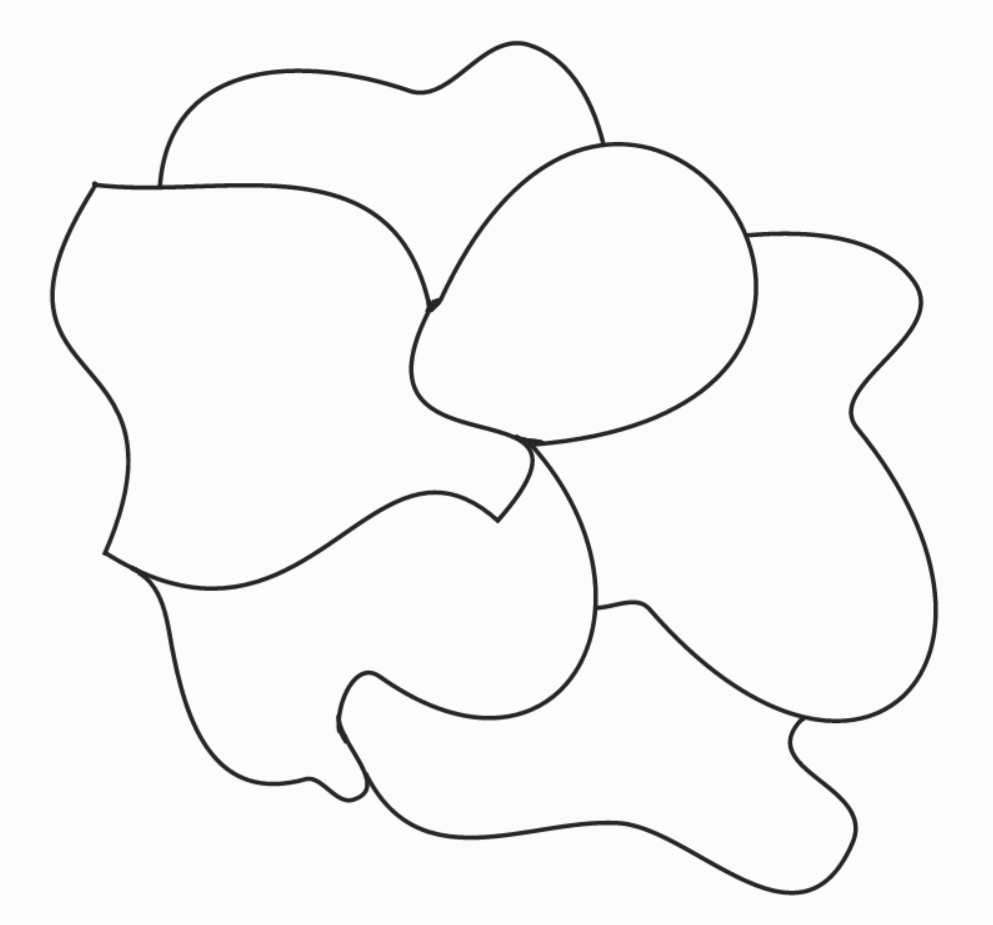
\includegraphics[width=0.5\textwidth]{Mappavuota.jpg}}; 
    		\begin{scope}[x={(image.south east)},y={(image.north west)}]
    			\node[circle, draw, fill=blue] (a) at (0.17,0.8) {};
    			\node[circle, draw, fill=blue] (b) at (0.61,0.84) {};
    			\node[circle, draw, fill=blue] (c) at (0.43,0.67) {};
    			\node[circle, draw, fill=blue] (d) at (0.75,0.75) {};
    			\node[circle, draw, fill=blue] (e) at (0.54,0.52) {};
    			\node[circle, draw, fill=blue] (f) at (0.14,0.39) {};
    			\node[circle, draw, fill=blue] (g) at (0.6,0.34) {};
    			\node[circle, draw, fill=blue] (h) at (0.36,0.18) {};
    			\node[circle, draw, fill=blue] (i) at (0.81,0.23) {};
    			
    			\draw[blue, thick] (a) -- (b) -- (c) -- (a) -- (f) -- (e) -- (c);
    			\draw[blue, thick] (f) -- (h) -- (g) -- (e) -- (d) -- (b);
    			\draw[blue, thick] (h) -- (i) -- (g);
    			\draw[blue, thick] (i) -- (d);
    		\end{scope}
    	\end{tikzpicture}
    	\caption{Nel grafo $G$ (rappresentato in blu) ogni vertice corrisponde a un punto di intersezione tra le frontiere delle regioni di $\mathcal{M}$ e gli archi sostituiscono i lati delle regioni.}
    	\label{fig:mappavuota}
    \end{figure}
    \\A questo punto, possiamo costruire il grafo $G^*$ come duale di $G$.
    \begin{figure}[h]
    	\centering
    	\begin{tikzpicture}[scale=0.8]
    	    \node[circle, draw, fill=blue] (a) at (1.7,8) {};
    	    \node[circle, draw, fill=blue] (b) at (6.1,8.4) {};
    	    \node[circle, draw, fill=blue] (c) at (4.3,6.7) {};
    	    \node[circle, draw, fill=blue] (d) at (7.5,7.5) {};
    	    \node[circle, draw, fill=blue] (e) at (5.4,5.2) {};
    	    \node[circle, draw, fill=blue] (f) at (1.4,3.9) {};
    	    \node[circle, draw, fill=blue] (g) at (6,3.4) {};
    	    \node[circle, draw, fill=blue] (h) at (3.6,1.8) {};
    	    \node[circle, draw, fill=blue] (i) at (8.1,2.3) {};
    	    
    	    \node[circle, draw, fill=red] (A) at (4.2,7.7) {};
    	    \node[circle, draw, fill=red] (B) at (3.2,5.6) {};
    	    \node[circle, draw, fill=red] (C) at (6,6.8) {};
    	    \node[circle, draw, fill=red] (D) at (4,3.5) {};
    	    \node[circle, draw, fill=red] (E) at (7,4.4) {};
    	    \node[circle, draw, fill=red] (F) at (6,2.6) {};
    	    
    	    \draw[blue, thick] (a) -- (b) -- (c) -- (a) -- (f) -- (e) -- (c);
    	    \draw[blue, thick] (f) -- (h) -- (g) -- (e) -- (d) -- (b);
    	    \draw[blue, thick] (h) -- (i) -- (g);
    	    \draw[blue, thick] (i) -- (d);	
    	    
    	    \draw[red, thick] (B) -- (A) -- (C) -- (B) -- (D) -- (E) -- (F) -- (D);
    	    \draw[red, thick] (C) -- (E);
    	\end{tikzpicture}
    	\vspace{0.5cm}
        \caption{Il grafo $G^*$ (rappresentato in rosso) è il duale di $G$ (e quindi di $\mathcal{M}$). In questo caso non è rappresentato il nodo corrispondente alla faccia illimitata, poiché solitamente la colorazione riguarda soltanto le facce interne. Qualora non fosse così, sarebbe sufficiente aggiungere un altro nodo adiacente ai 6 già rappresentati.}
    \end{figure}
    
    \noindent \emph{Note}: La mappa di partenza $\mathcal{M}$ è una mappa planare, di conseguenza anche il grafo duale $G^*$ sarà planare.
    \\Inoltre, $G^*$ non può contenere cappi, in quanto una regione non può confinare con sé stessa, e nemmeno archi paralleli, poiché una relazione di adiacenza tra due regioni produce un unico arco tra i nodi corrispondenti, di conseguenza $G^*$ è anche semplice.
    % esempio
    
    \section{Il Teorema dei Quattro Colori}
    Giunti a questo punto della tesi, dopo aver affrontato la storia del Teorema e aver fornito le definizioni necessarie, abbiamo tutti gli strumenti fondamentali per poter formulare il Teorema dei Quattro Colori utilizzando la Teoria dei Grafi e comprenderne la dimostrazione, trattata nel capitolo 5.
    \begin{namedthm*}{Teorema dei Quattro Colori (Appel e Haken, 1976)}
    	Dato un grafo $G$ semplice e planare, $\chi(G) \leq 4$.
    \end{namedthm*}
    \noindent In altre parole, il numero cromatico di un grafo semplice planare $\chi(G)$ è sempre minore o uguale a 4, perciò tutti i grafi di questo tipo sono 4-colorabili.
    \\Naturalmente, l'enunciato è equivalente a quello fornito nella sezione 2.1, poiché ogni grafo semplice planare può essere considerato il duale di una mappa planare e una 4-colorazione dei nodi del grafo corrisponde a una 4-colorazione delle regioni della mappa.
    È possibile passare in modo semplice da una mappa planare al proprio grafo duale, come visto nella sezione 3.2, e allo stesso modo passare da un grafo semplice planare alla propria mappa duale, seguendo il metodo inverso, ossia trasformando i nodi in regioni e gli archi in lati di confine.
    \\Prima di affrontare la dimostrazione del Teorema, chiariamo che esistono naturalmente grafi con numero cromatico 1, 2 o 3, quindi colorabili con meno di 4 colori ed evidentemente non tra i casi "critici", che possano mettere in dubbio la validità del Teorema.
    \begin{figure}[h]
    	\centering
    	\begin{tikzpicture}
    		\node[circle, draw, fill=blue] (a) at (0,0) {};
    		\node[circle, draw, fill=blue] (b) at (1.2,0.8) {};
    		\node[circle, draw, fill=blue] (c) at (1.5,-0.6) {};
    		
    		\node[circle, draw, fill=green] (d) at (3.5,0.2) {};
    		\node[circle, draw, fill=red] (e) at (4.8,1.1) {};
    		\node[circle, draw, fill=green] (f) at (5.5,0) {};
    		\node[circle, draw, fill=red] (g) at (4.2,-0.9) {};
    		\draw (d) -- (e) -- (f) -- (g)  -- (d);
    		
    		\node[circle, draw, fill=blue] (A) at (7.5,0) {};
    		\node[circle, draw, fill=red] (B) at (8.7,1.2) {};
    		\node[circle, draw, fill=blue] (C) at (9.8,0.4) {};
    		\node[circle, draw, fill=red] (D) at (9.2,-0.8) {};
    		\node[circle, draw, fill=green] (E) at (8.2,-1) {};
    		\draw (A) -- (B) -- (C) -- (D) -- (E) -- (A);
        \end{tikzpicture}
        \vspace{0.4cm}
        \caption{3 grafi $G_1$, $G_2$ e $G_3$, con $\chi(G_1) = 1$, $\chi(G_2) = 2$ e $\chi(G_3) = 3$.}
    \end{figure}
    \\Proviamo con due semplici esempi che tuttavia esistono effettivamente grafi che sono 4-colorabili, ma non 3-colorabili, e che di conseguenza non può esistere un "Teorema dei Tre Colori" poiché i colori utilizzati in questi controesempi devono essere almeno 4. 
    	\begin{figure}[h]
    	\centering
    	\begin{tikzpicture}
    		\node[circle, draw, fill=yellow!70] (A) at (0, 1.5) {};
    		\node[circle, draw, fill=green!70] (B) at (1.5, -1) {};
    		\node[circle, draw, fill=red!70] (C) at (-1.5, -1) {};
    		\node[circle, draw, fill=blue!70] (O) at (0, 0) {};
    		
    		\draw (A) -- (B) -- (C) -- (A); 
    		\draw (O) -- (A);
    		\draw (O) -- (B);
    		\draw (O) -- (C);
    	\end{tikzpicture}
    	\hspace{2cm} 
    	\begin{tikzpicture}
    		\node[circle, draw, fill=yellow!70] (A) at (0, 1.5) {};
    		\node[circle, draw, fill=green!70] (B) at (1.43, 0.47) {};
    		\node[circle, draw, fill=red!70] (C) at (0.88, -1.21) {};
    		\node[circle, draw, fill=yellow!70] (D) at (-0.88, -1.21) {};
    		\node[circle, draw, fill=red!70] (E) at (-1.43, 0.47) {};
    		\node[circle, draw, fill=blue!70] (O) at (0, 0) {};
    		
    		\draw (A) -- (B) -- (C) -- (D) -- (E) -- (A); 
    		\draw (O) -- (A);
    		\draw (O) -- (B);
    		\draw (O) -- (C);
    		\draw (O) -- (D);
    		\draw (O) -- (E);
    	\end{tikzpicture}
    	\vspace{0.5cm}
    	\caption{I due esempi minimi di grafi 4-colorabili, ma non 3-colorabili.}
    \end{figure}
    	
    \chapter{Le dimostrazioni di Kempe e Heawood}
    
    In questo capitolo ripercorriamo in modo dettagliato la dimostrazione errata del Teorema dei Quattro Colori pubblicata da Kempe e la dimostrazione del Teorema dei Cinque Colori individuata da Heawood.
    \section{La dimostrazione errata di Kempe}
    La "dimostrazione" del Teorema dei Quattro Colori di Kempe ({\bfseries \cite{Kempe}} e {\bfseries \cite{Simonson}}) è una dimostrazione per induzione sul numero dei nodi e fornisce un algoritmo ricorsivo per la colorazione dei vertici.
    \\Kempe si propone di dimostrare che se ogni grafo $G = (V,E)$ con $\lvert V \rvert = n$ nodi è 4-colorabile, allora lo è anche ogni grafo con $n + 1$ nodi.
    \\Per comprendere la dimostrazione di Kempe è fondamentale introdurre una formula, nota come Formula di Eulero, che fornisce una relazione tra il numero di nodi, archi e facce in un grafo planare connesso.
    \begin{namedthm*}{Formula di Eulero}
    	Se $G$ è un grafo planare connesso, allora vale la relazione 
    	\\$\lvert V \rvert - \lvert E \rvert + \lvert F \rvert = 2$, dove
    	\begin{itemize}
    		\item $V$ è l'insieme dei nodi di $G$
    		\item $E$ è l'insieme degli archi di $G$
    		\item $F$ è l'insieme delle facce di $G$.
    	\end{itemize}
    \end{namedthm*}
    \begin{proof}
        Utilizziamo per comodità $V$, $E$ ed $F$ al posto di $\lvert V \rvert$, $\lvert E \rvert$, ed $\lvert F \rvert$ e dimostriamo la formula per induzione sul numero di archi $E$:
        \\(\emph{Caso base}) Sia $E = 0$. 
        \\Allora il grafo $G$ ha un solo vertice (altrimenti sarebbe vuoto) e una sola faccia, costituita da tutto il piano, perciò $V = 1$ e $F = 1$.	
        \\Di conseguenza $V - E + F = 1 - 0 + 1 = 2$ e la Formula di Eulero è verificata.
        \\(Passo induttivo) Supponiamo che la Formula sia valida per $E = n$.
        \\Sia $E = n + 1$. Ci sono due possibili casi:
        \begin{enumerate}
        	\item $G$ contiene un vertice $v$ di grado 1.
        	\\Eliminiamo il vertice $v$ e l'unico arco incidente ad esso, ottenendo un grafo $G' = G \smallsetminus v$ con $V' = V - 1$, $E' = E - 1 = n$, $F' = F$.
        	\\Per ipotesi vale quindi $V' - E' + F' = 2$, perciò $V - 1 - E + 1 + F = V - E + F = 2$.
        	\item $G$ non contiene vertici di grado 1.
        	\\Ogni arco fa necessariamente parte del perimetro di una faccia (non quella esterna), scegliamo un arco, che chiamiamo $e$, lo rimuoviamo e otteniamo un grafo $G' = G \smallsetminus e$ con $V' = V$, $E' = E - 1 = n$, $F' = F - 1$.
        	\\Per ipotesi vale $V' - E' + F' = 2$, perciò $V - E + 1 + F - 1 = V - E + F = 2$. \qedhere
        \end{enumerate}
    \end{proof}
       Sappiamo dunque che, per ogni grafo $G$, vale $V - E + F = 2$ per la Formula di Eulero, inoltre ogni faccia del grafo è delimitata da almeno 3 archi, ciascuno dei quali appartiene al perimetro di due facce, vale dunque la relazione $3F \leq 2E$, perciò $F \leq \frac{2E}{3}$.
    \\Risolviamo quindi il sistema
    \[
    \begin{cases}
    	F \leq \frac{2E}{3}\\
    	V - E + F = 2
    \end{cases}
    \] 
    e otteniamo $2 = V - E + F \leq V - E + \frac{2E}{3}$.
    \\Perciò $V - \frac{E}{3} \geq 2$, da cui si ottiene $E \leq 3V - 6$.
    \\Questa formula è valida per ogni grafo planare e può essere sfruttata per dimostrare il seguente Lemma, fondamentale nello sviluppo successivo della dimostrazione di Kempe:
    \begin{namedthm*}{Lemma 4.1}
    	Ogni grafo planare contiene almeno un vertice $v$ tale che $\deg(v) \leq 5$.
    \end{namedthm*}
    \begin{proof}[Dimostrazione (Lemma 4.1)]
    	Dato che in un grafo ogni arco è incidente a due vertici, vale la relazione 
    	\[
    	\sum_{v \in V} \deg(v) = 2E.
    	\]
    	Ma come abbiamo appena visto, vale anche $E \leq 3V - 6$, e di conseguenza $2E \leq 6V - 12$. Quindi 
    	\[
    	\sum_{v \in V} \deg(v) \leq 6V - 12.
    	\]
    	Supponiamo per assurdo che $\deg(v) \geq 6$ $\forall v \in V$.
    	Allora abbiamo che
    	\[
    	\begin{cases}
    		\sum_{v \in V} \deg(v) \geq 6V\\
    		\sum_{v \in V} \deg(v) \leq 6V - 12
    	\end{cases}
    	\] 	
    	Perciò $6V - 12 \geq 6V$, che è chiaramente una contraddizione.
    	\\Di conseguenza, almeno un vertice $v \in V$ è tale che $\deg(v) \leq 5$.
    \end{proof}
    Ricordiamo ora la Congettura dei Quattro Colori e passiamo alla vera e propria dimostrazione (errata) di Kempe.
    \begin{namedthm*}{Congettura dei Quattro Colori}
    	Se $G$ è un grafo semplice e planare, $\chi(G) \leq 4$.
    \end{namedthm*}
    \begin{proof}[Dimostrazione (con errore)]
        \noindent Procediamo per induzione sul numero di vertici:
        \\(\emph{Caso base}) Sappiamo che se $G = (V,E)$ è un grafo con $\lvert V \rvert \leq 4$, allora esso è colorabile con al più 4 colori: è sufficiente utilizzare un colore diverso per ogni vertice.
        % esempio?
        \\(\emph{Passo induttivo}) Supponiamo che ogni grafo con $\lvert V \rvert = n$ sia 4-colorabile, dimostriamo allora che anche ogni grafo con $\lvert V \rvert = n + 1$ è 4-colorabile.
        \\Consideriamo quindi un grafo $G = (V, E)$ con $\lvert V \rvert = n + 1$, individuiamo in esso un vertice $v \in V$ tale che $\deg(v) \leq 5$, che esisterà sicuramente, come dimostrato in precedenza, e rimuoviamolo da $G$, ottenendo un grafo $G \smallsetminus v$.
        \\$G \smallsetminus v$ ha $n$ nodi, perciò è 4-colorabile, coloriamo quindi $G \smallsetminus v$ con 4 colori e reinseriamo in esso il vertice $v$ con i relativi archi incidenti: sarà sufficiente colorare $v$ per ottenere una 4-colorazione di $G$, provando quindi la Congettura.
        \\Il vertice $v$ può avere grado 1, 2, 3, 4 o 5, consideriamo quindi 5 casi e utilizziamo ad esempio i colori rosso, blu, verde e giallo.
        \begin{enumerate}
        	\item $\deg(v) = 1$:
        	\\$v$ ha un solo nodo adiacente, colorato con un colore, quindi è sufficiente utilizzare un colore differente per $v$.
        	\begin{figure}[H]
        		\centering
        		\begin{tikzpicture}
        			\node[circle, draw] (v) at (-1,-0.5) {$v$};
        			\node[circle, draw, fill=blue!50] (B) at (1,0.5) {B};
        			
        			\draw (v) -- (B);
        			
        			\draw[->, thick] (2,-0.1) -- (4,-0.1);
        			
        			\node[circle, draw, fill=red!50] (v1) at (5,-0.5) {$v$};
        			\node[circle, draw, fill=blue!50] (B1) at (7,0.5) {B};
        			
        			\draw (v1) -- (B1);
        		\end{tikzpicture}
        		\vspace{0.5cm}
        		\caption{$\deg(v) = 1$: il nodo B, adiacente a $v$, è colorato di blu, quindi $v$ può essere colorato di rosso (oppure verde o giallo).}
        	\end{figure}
        	\item $\deg(v) = 2$:
        	\\$v$ ha soltanto 2 nodi adiacenti, colorati con, al più, 2 colori diversi. \\Utilizziamo semplicemente un colore diverso per $v$ e abbiamo terminato.
        	\begin{figure}[H]
        		\centering
        		\begin{tikzpicture}
        			\node[circle, draw] (v) at (0,0) {$v$};
        			\node[circle, draw, fill=blue!50] (B) at (1,1) {B};
        			\node[circle, draw, fill=red!50] (R) at (1,-1) {R};
        			
        			\draw (v) -- (B);
        			\draw (v) -- (R);
        			
        			\draw[->, thick] (2,0) -- (4,0);
        			
        			\node[circle, draw, fill=yellow!50] (v1) at (5,0) {$v$};
        			\node[circle, draw, fill=blue!50] (B1) at (6,1) {B};
        			\node[circle, draw, fill=red!50] (R1) at (6,-1) {R};
        			
        			\draw (v1) -- (B1);
        			\draw (v1) -- (R1);
        		\end{tikzpicture}
        		\vspace{0.5cm}
        		\caption{$\deg(v) = 2$: i nodi B ed R, adiacenti a $v$, sono colorati di blu e rosso, quindi $v$ può essere colorato di giallo (o verde).}
        	\end{figure}
        	\item $\deg(v) = 3$:
        	\\$v$ ha 3 nodi adiacenti, colorati con, al più, 3 colori diversi. 
        	\\Come nei casi precedenti, utilizziamo un colore diverso per $v$ e abbiamo terminato.
        	\begin{figure}[H]
        		\centering
        		\begin{tikzpicture}
        			\node[circle, draw] (v) at (0,0) {$v$};
        			\node[circle, draw, fill=blue!50] (B) at (0,1.5) {B};
        			\node[circle, draw, fill=yellow!50] (G) at (-1.5,-1) {G};
        			\node[circle, draw, fill=red!50] (R) at (1.5,-1) {R};
        			
        			\draw (v) -- (B);
        			\draw (v) -- (G);
        			\draw (v) -- (R);
        			
        			\draw[->, thick] (2.5,0) -- (4.5,0);
        			
        			\node[circle, draw, fill=green!50] (v1) at (7,0) {$v$};
        			\node[circle, draw, fill=blue!50] (B1) at (7,1.5) {B};
        			\node[circle, draw, fill=yellow!50] (G1) at (5.5,-1) {G};
        			\node[circle, draw, fill=red!50] (R1) at (8.5,-1) {R};
        			
        			\draw (v1) -- (B1);
        			\draw (v1) -- (G1);
        			\draw (v1) -- (R1);
        		\end{tikzpicture}
        		\vspace{0.5cm}
        		\caption{$\deg(v) = 3$: i nodi B, R e G, adiacenti a $v$, sono colorati di blu, rosso e giallo, quindi $v$ può essere colorato di verde.}
        	\end{figure}
        	\item $\deg(v) = 4$:
        	\\Questo è il primo caso non banale, poiché i 4 vertici adiacenti a $v$ potrebbero essere colorati con 4 colori diversi, rendendo quindi necessario un metodo per modificarne la colorazione.
        	\\Qualora invece i colori utilizzati siano meno di 4, è sufficiente seguire l'esempio dei casi 1, 2 e 3 e colorare $v$.
        	\\Allo scopo di risolvere il caso non banale definiamo il significato di \emph{catena di Kempe}.
        	\begin{dfn}
        		In un grafo $G = (V, E)$ con una colorazione propria dei vertici, dati due colori $c_1$ e $c_2$, una {\bfseries catena di Kempe} (\emph{Kempe chain}) $c_1$-$c_2$ è un sottografo bipartito e connesso $K = (C_1 \cup C_2, E')$ tale che ogni vertice di $C_1$ sia colorato con il colore $c_1$ e ogni vertice di $C_2$ sia colorato con il colore $c_2$.
        		\\Se ad esempio vogliamo determinare la catena di Kempe rossa-blu che contiene uno specifico vertice rosso, individuiamo tutti i vertici blu ad esso adiacenti, tutti i vertici rossi adiacenti ad ognuno di questi e così via.
        	\end{dfn}
        	\begin{figure}[h]
        		\centering
        		\begin{tikzpicture}
        			\node[circle, draw, fill=blue!60] (a) at (0,0) {};
        			\node[circle, draw, fill=red!60] (b) at (1,1) {};
        			\node[circle, draw, fill=blue!60] (c) at (2.5,0.5) {};
        			\node[circle, draw, fill=red!60] (d) at (0.5,-1) {};
        			\node[circle, draw, fill=blue!60] (e) at (3,2) {};
        			\node[circle, draw, fill=red!60] (f) at (3.2,-0.5) {};
        			\node[circle, draw, fill=blue!60] (g) at (4.2,0.3) {};
        			\node[circle, draw, fill=red!60] (h) at (5.2,1.5) {};
        			\node[circle, draw, fill=blue!60] (i) at (0.2,2.5) {};
        			\node[circle, draw, fill=red!60] (j) at (5,2.3) {};
        			
        			\draw (d) -- (a) -- (b) -- (c) -- (f) -- (g);
        			\draw (e) -- (j);
        			\draw (i) -- (b) -- (e) -- (h);
        		\end{tikzpicture}
        		\vspace{0.5cm}
        		\caption{Catena di Kempe rossa-blu.}
        	\end{figure}
        	Supponiamo, senza perdita di generalità, che i 4 vertici adiacenti a $v$ siano colorati con i colori rosso, giallo, verde e blu, in senso orario, e chiamiamoli rispettivamente R, G, V e B.
        	\begin{figure}[H]
        		\centering
        		\begin{tikzpicture}
        			\node[circle, draw] (v) at (0,0) {$v$};
        			\node[circle, draw, fill=red!50] (R) at (0.2,1.8) {R};
        			\node[circle, draw, fill=yellow!50] (G) at (2.3,0.3) {G};
        			\node[circle, draw, fill=green!50] (V) at (0.4,-1.7) {V};
        			\node[circle, draw, fill=blue!50] (B) at (-1.7,-0.6) {B};
        			
        			\draw (B) -- (v) -- (G);
        			\draw (R) -- (v) -- (V);
        		\end{tikzpicture}
        		\vspace{0.5cm}
        		\caption{$\deg(v) = 4$, i 4 vertici adiacenti a $v$ sono colorati con 4 colori diversi.}
        	\end{figure}
        	Consideriamo allora due sottocasi:
        	\begin{description}
        		\item[i)] La catena di Kempe blu-gialla che contiene B non contiene anche G:
        		\\in questo caso è sufficiente invertire i colori nella catena di Kempe, da blu a giallo e da giallo a blu, il vertice B diventerà giallo, come G, e quindi $v$ potrà essere colorato di blu.
        		\\Sottolineiamo che invertire i colori nella catena di Kempe consente di mantenere una colorazione propria del grafo, poiché se il colore di un vertice viene modificato da blu a giallo, ogni vertice giallo ad esso adiacente viene a sua volta colorato di blu, e viceversa.
        			\begin{figure}[h]
        			\centering
        			\resizebox{\textwidth}{!}{
        			\begin{tikzpicture}
        				\node[circle, draw] (v) at (0,0) {$v$};
        				\node[circle, draw, fill=red!50] (R) at (0.2,1.8) {R};
        				\node[circle, draw, fill=yellow!50] (G) at (2.3,0.3) {G};
        				\node[circle, draw, fill=green!50] (V) at (0.4,-1.7) {V};
        				\node[circle, draw, fill=blue!50] (B) at (-1.7,-0.6) {B};
        				\node[circle, draw, fill=yellow!50] (G1) at (-3,0.2) {};
        				\node[circle, draw, fill=blue!50] (B1) at (-4,-0.4) {};
        				\node[circle, draw, fill=yellow!50] (G2) at (-3.6,-1.8) {};
        				\node[circle, draw, fill=blue!50] (B2) at (-2.6,-2.5) {};
        				\node[circle, draw, fill=yellow!50] (G3) at (-1.3,-2) {};
        				
        				\draw (B) -- (v) -- (G);
        				\draw (R) -- (v) -- (V);
        				\draw (G3) -- (B) -- (G1) -- (B2) -- (G2);
        				\draw (G1) -- (B1);
        				
        				\draw[->, thick] (3.3,0) -- (5.3,0);
        				
        				\node[circle, draw, fill=blue!50] (v') at (10.3,0) {$v$};
        				\node[circle, draw, fill=red!50] (R') at (10.5,1.8) {R};
        				\node[circle, draw, fill=yellow!50] (G') at (12.6,0.3) {G};
        				\node[circle, draw, fill=green!50] (V') at (10.7,-1.7) {V};
        				\node[circle, draw, fill=yellow!50] (B') at (8.6,-0.6) {B};
        				\node[circle, draw, fill=blue!50] (G1') at (7.3,0.2) {};
        				\node[circle, draw, fill=yellow!50] (B1') at (6.3,-0.4) {};
        				\node[circle, draw, fill=blue!50] (G2') at (6.7,-1.8) {};
        				\node[circle, draw, fill=yellow!50] (B2') at (7.7,-2.5) {};
        				\node[circle, draw, fill=blue!50] (G3') at (9,-2) {};
        				
        				\draw (B') -- (v') -- (G');
        				\draw (R') -- (v') -- (V');
        				\draw (G3') -- (B') -- (G1') -- (B2') -- (G2');
        				\draw (G1') -- (B1');
        			\end{tikzpicture}
        		}
        			\vspace{0.5cm}
        			\caption{Inversione dei colori nella catena di Kempe blu-gialla contenente B. In questo modo $v$ può essere colorato di blu.}
        		\end{figure}
        		\item[ii)] La catena di Kempe blu-gialla che contiene B contiene anche G (\emph{catena di Kempe ciclica}):
        		\clearpage
        			\begin{figure}[h]
        			\centering
        			\begin{tikzpicture}
        				\node[circle, draw] (v) at (0,0) {$v$};
        				\node[circle, draw, fill=red!50] (R) at (0.2,1.8) {R};
        				\node[circle, draw, fill=yellow!50] (G) at (2.3,0.3) {G};
        				\node[circle, draw, fill=green!50] (V) at (0.4,-1.7) {V};
        				\node[circle, draw, fill=blue!50] (B) at (-1.7,-0.6) {B};
        				
        				\node[circle, draw, fill=yellow!50] (G1) at (-3,0.2) {};
        				\node[circle, draw, fill=blue!50] (B1) at (-4,-0.4) {};
        				\node[circle, draw, fill=yellow!50] (G2) at (-3.6,-1.8) {};
        				\node[circle, draw, fill=blue!50] (B2) at (-2.6,-2.5) {};
        				\node[circle, draw, fill=yellow!50] (G3) at (-1.3,-2) {};
        				
        				\node[circle, draw, fill=blue!50] (B3) at (1.7,-1.5) {};
        				\node[circle, draw, fill=yellow!50] (G4) at (2,-2.2) {};
        				\node[circle, draw, fill=blue!50] (B4) at (2.6,-1) {};
        				\node[circle, draw, fill=yellow!50] (G5) at (1.4,-3.2) {};
        				
        				\draw (B) -- (v) -- (G);
        				\draw (R) -- (v) -- (V);
        				\draw (G3) -- (B) -- (G1) -- (B2) -- (G2);
        				\draw (G1) -- (B1);
        				\draw (G) -- (B3) -- (G4) -- (B4) -- (G);
        				\draw (B3) -- (G5);
        				
        				\draw[line width=2pt, yellow] (B2) -- (G5);
        				\draw[dashed, line width=2pt, blue] (B2) -- (G5);
        			\end{tikzpicture}
        			\vspace{0.5cm}
        			\caption{Catena di Kempe ciclica tra B e G.
        				\\La linea blu-gialla indica vertici blu e gialli che fanno parte della catena.}
        		\end{figure}
        		Questo caso è leggermente più complesso, poiché il metodo illustrato precedentemente scambierebbe soltanto il colore di G e di B, poiché appartengono alla stessa catena di Kempe, senza risolvere il problema.
        		\\Tuttavia, se la catena gialla-blu è ciclica, significa che esiste un cammino giallo-blu tra G e B, ma di conseguenza non può esistere un cammino rosso-verde tra R e V, in quanto, per la proprietà di planarità del grafo, ogni cammino tra R e V deve contenere almeno un vertice blu o giallo appartenente alla catena ciclica blu-gialla, quindi la catena di Kempe rossa-verde che contiene R non è ciclica.
        		\\Possiamo allora applicare il metodo del caso precedente a R, colorarlo di verde, proprio come V, liberando quindi il colore rosso per $v$.
        		\begin{figure}[h]
        			\centering
        			\begin{tikzpicture}
        				\node[circle, draw] (v) at (0,0) {$v$};
        				\node[circle, draw, fill=red!50] (R) at (0.2,1.8) {R};
        				\node[circle, draw, fill=yellow!50] (G) at (2.3,0.3) {G};
        				\node[circle, draw, fill=green!50] (V) at (0.4,-1.7) {V};
        				\node[circle, draw, fill=blue!50] (B) at (-1.7,-0.6) {B};
        				
        				\node[circle, draw, fill=green!50] (V1) at (-1.5,2.3) {};
        				\node[circle, draw, fill=red!50] (R1) at (-1.2,1.2) {};
        				\node[circle, draw, fill=green!50] (V2) at (2.8,1.5) {};
        				\node[circle, draw, fill=red!50] (R2) at (1.2,2.8) {};
        				
        				\draw (B) -- (v) -- (G);
        				\draw (R) -- (v) -- (V);
        				
        				\draw (R1) -- (V1) -- (R2) -- (V2);
        				\draw (R) -- (V1);
        				
        				\draw[line width=2pt, blue] (B) .. controls (-0.3,-2.9) and (1.5,-2.9) .. (G);
        				\draw[dashed, line width=2pt, yellow] (B) .. controls (-0.3,-2.9) and (1.5,-2.9) .. (G);
        				
        				\draw[->, thick] (3.8,0) -- (5.8,0);
        				
        				\node[circle, draw, fill=red!50] (v') at (8.5,0) {$v$};
        				\node[circle, draw, fill=green!50] (R') at (8.7,1.8) {R};
        				\node[circle, draw, fill=yellow!50] (G') at (10.8,0.3) {G};
        				\node[circle, draw, fill=green!50] (V') at (8.9,-1.7) {V};
        				\node[circle, draw, fill=blue!50] (B') at (6.8,-0.6) {B};
        				
        				\node[circle, draw, fill=red!50] (V1') at (7,2.3) {};
        				\node[circle, draw, fill=green!50] (R1') at (7.3,1.2) {};
        				\node[circle, draw, fill=red!50] (V2') at (11.3,1.5) {};
        				\node[circle, draw, fill=green!50] (R2') at (9.7,2.8) {};
        				
        				\draw (B') -- (v') -- (G');
        				\draw (R') -- (v') -- (V');
        				
        				\draw (R1') -- (V1') -- (R2') -- (V2');
        				\draw (R') -- (V1');
        				
        				\draw[line width=2pt, blue] (B') .. controls (8.2,-2.9) and (10,-2.9) .. (G');
        				\draw[dashed, line width=2pt, yellow] (B') .. controls (8.2,-2.9) and (10,-2.9) .. (G');
        			\end{tikzpicture}
        			\vspace{0.5cm}
        			\caption{Inversione dei colori nella catena di Kempe rossa-verde (necessariamente non ciclica) contenente R. In questo modo $v$ può essere colorato di rosso.}
        		\end{figure}
        	\end{description}
        	\emph{Nota}: fino a questo punto la dimostrazione di Kempe non presenta alcun errore.
        	\item $\deg(v) = 5$:
        	\\Questo è il caso più complicato. Naturalmente, se i colori utilizzati per i nodi adiacenti a $v$ sono meno di 4, scegliamo un colore per $v$ e abbiamo terminato, come nei casi 1,2 e 3.
        	\\Consideriamo il caso in cui i colori già utilizzati sono invece 4, allora due dei 5 vertici avranno lo stesso colore.
        	\\Scegliamo ad esempio il rosso come colore ripetuto e individuiamo 2 sottocasi:
        	\begin{description}
        		\item[i)] I vertici rossi sono consecutivi in sequenza l'uno all'altro:
        		\\ad esempio assegniamo i colori verde, giallo, blu, rosso e di nuovo rosso in senso orario, chiamiamo i vertici rispettivamente V, G, B, R\textsubscript{1} ed R\textsubscript{2}.
        		\begin{figure}[h]
        			\centering
        			\begin{tikzpicture}
        				\node[circle, draw] (v) at (0,0) {$v$};
        				\node[circle, draw, fill=green!50] (V) at (0.2,1.8) {V};
        				\node[circle, draw, fill=yellow!50] (G) at (2.3,0.3) {G};
        				\node[circle, draw, fill=blue!50] (B) at (0.4,-1.7) {B};
        				\node[circle, draw, fill=red!50] (R1) at (-1.5,-0.8) {R\textsubscript{1}};
        				\node[circle, draw, fill=red!50] (R2) at (-2.2,0.6) {R\textsubscript{2}};
        				
                        \draw (B) -- (v) -- (V);
        				\draw (R1) -- (v) -- (G);
        				\draw (R2) -- (v);
        			\end{tikzpicture}
        			\vspace{0.5cm}
        			\caption{$\deg(v) = 5$, i 5 vertici adiacenti a $v$ sono colorati con 4 colori diversi. \\I vertici R\textsubscript{1} ed R\textsubscript{2}, entrambi rossi, sono consecutivi.}
        		\end{figure}
        		\\Questo caso è molto simile a quello precedente: individuiamo la catena di Kempe verde-blu contenente V, se non è ciclica invertiamo tutti i colori dei vertici al suo interno, V sarà quindi colorato di blu, come B, e il colore verde sarà disponibile per $v$.
        		\begin{figure}[h]
        			\centering
        			\begin{tikzpicture}
        				\node[circle, draw] (v) at (0,0) {$v$};
        				\node[circle, draw, fill=green!50] (V) at (0.2,1.8) {V};
        				\node[circle, draw, fill=yellow!50] (G) at (2.3,0.3) {G};
        				\node[circle, draw, fill=blue!50] (B) at (0.4,-1.7) {B};
        				\node[circle, draw, fill=red!50] (R1) at (-1.5,-0.8) {R\textsubscript{1}};
        				\node[circle, draw, fill=red!50] (R2) at (-2.2,0.6) {R\textsubscript{2}};
        				
        				\node[circle, draw, fill=green!50] (V1) at (-1.5,2.3) {};
        				\node[circle, draw, fill=blue!50] (B2) at (2.6,3.2) {};
        				\node[circle, draw, fill=green!50] (V2) at (2.8,1.5) {};
        				\node[circle, draw, fill=blue!50] (B1) at (1.2,2.8) {};
        				
        				\draw (B) -- (v) -- (V);
        				\draw (R1) -- (v) -- (G);
        				\draw (R2) -- (v);
        				\draw (V1) -- (B1) -- (V2) -- (B2);
        				\draw (V) -- (B1);
        				
        				\draw[->, thick] (3.8,0) -- (5.8,0);
        				
        				\node[circle, draw, fill=green!50] (v') at (9,0) {$v$};
        				\node[circle, draw, fill=blue!50] (V') at (9.2,1.8) {V};
        				\node[circle, draw, fill=yellow!50] (G') at (11.3,0.3) {G};
        				\node[circle, draw, fill=blue!50] (B') at (9.4,-1.7) {B};
        				\node[circle, draw, fill=red!50] (R1') at (7.5,-0.8) {R\textsubscript{1}};
        				\node[circle, draw, fill=red!50] (R2') at (6.8,0.6) {R\textsubscript{2}};
        				
        				\node[circle, draw, fill=blue!50] (V1') at (7.5,2.3) {};
        				\node[circle, draw, fill=green!50] (B2') at (11.6,3.2) {};
        				\node[circle, draw, fill=blue!50] (V2') at (11.8,1.5) {};
        				\node[circle, draw, fill=green!50] (B1') at (10.2,2.8) {};
        				
        				\draw (B') -- (v') -- (V');
        				\draw (R1') -- (v') -- (G');
        				\draw (R2') -- (v');
        				\draw (V1') -- (B1') -- (V2') -- (B2');
        				\draw (V') -- (B1');
        			\end{tikzpicture}
        			\vspace{0.5cm}
        			\caption{Inversione dei colori nella catena di Kempe (non ciclica) verde-blu contenente V. In questo modo $v$ può essere colorato di verde.}
        		\end{figure}
        		\\Se la catena è ciclica e quindi contiene V e B, individuiamo la catena di Kempe gialla-rossa contenente G, essa non può essere ciclica né tra G ed R\textsubscript{1}, né tra G ed R\textsubscript{2}, perciò è sufficiente invertire i colori al suo interno, G verrà colorato di rosso, come R\textsubscript{1} ed R\textsubscript{2}, e $v$ potrà essere colorato di giallo.
        		\begin{figure}[h]
        			\centering
        			\begin{tikzpicture}
        				\node[circle, draw] (v) at (0,0) {$v$};
        				\node[circle, draw, fill=green!50] (V) at (0.2,1.8) {V};
        				\node[circle, draw, fill=yellow!50] (G) at (2.3,0.3) {G};
        				\node[circle, draw, fill=blue!50] (B) at (0.4,-1.7) {B};
        				\node[circle, draw, fill=red!50] (R1) at (-1.5,-0.8) {R\textsubscript{1}};
        				\node[circle, draw, fill=red!50] (R2) at (-2.2,0.6) {R\textsubscript{2}};
        				
        				\node[circle, draw, fill=red!50] (R3) at (1.8,1.5) {};
        				\node[circle, draw, fill=red!50] (R4) at (2.1,-1.8) {};
        				\node[circle, draw, fill=yellow!50] (G1) at (1,-0.6) {};
        				\node[circle, draw, fill=yellow!50] (G2) at (1.3,-2.7) {};
        				
        				\draw (B) -- (v) -- (V);
        				\draw (R1) -- (v) -- (G);
        				\draw (R2) -- (v);
        				\draw[line width=2pt, blue] (V) .. controls (-4.5,1.5) and (-4.5,-1.5) .. (B);
        				\draw[dashed, line width=2pt, green] (V) .. controls (-4.5,1.5) and (-4.5,-1.5) .. (B);
        				
        				\draw (R3) -- (G) -- (R4) -- (G1);
        				\draw (R4) -- (G2);
        				
        				\draw[->, thick] (3.3,0) -- (5.3,0);
        				
        				\node[circle, draw, fill=yellow!50] (v') at (9.3,0) {$v$};
        				\node[circle, draw, fill=green!50] (V') at (9.5,1.8) {V};
        				\node[circle, draw, fill=red!50] (G') at (11.6,0.3) {G};
        				\node[circle, draw, fill=blue!50] (B') at (9.7,-1.7) {B};
        				\node[circle, draw, fill=red!50] (R1') at (7.8,-0.8) {R\textsubscript{1}};
        				\node[circle, draw, fill=red!50] (R2') at (7.1,0.6) {R\textsubscript{2}};
        				
        				\node[circle, draw, fill=yellow!50] (R3') at (11.1,1.5) {};
        				\node[circle, draw, fill=yellow!50] (R4') at (11.4,-1.8) {};
        				\node[circle, draw, fill=red!50] (G1') at (10.3,-0.6) {};
        				\node[circle, draw, fill=red!50] (G2') at (10.6,-2.7) {};
        				
        				\draw (B') -- (v') -- (V');
        				\draw (R1') -- (v') -- (G');
        				\draw (R2') -- (v');
        				\draw[line width=2pt, blue] (V') .. controls (4.8,1.5) and (4.8,-1.5) .. (B');
        				\draw[dashed, line width=2pt, green] (V') .. controls (4.8,1.5) and (4.8,-1.5) .. (B');
        				
        				\draw (R3') -- (G') -- (R4') -- (G1');
        				\draw (R4') -- (G2');
        			\end{tikzpicture}
        			\vspace{0.5cm}
        			\caption{Inversione dei colori nella catena di Kempe gialla-rossa (necessariamente non ciclica) contenente G. In questo modo $v$ può essere colorato di giallo.}
        		\end{figure}
        		\item[ii)] I vertici rossi sono separati da un altro vertice:
        		consideriamo ad esempio la sequenza B-R\textsubscript{1}-G-V-R\textsubscript{2}, in senso orario.
        		\begin{figure}[h]
        			\centering
        			\begin{tikzpicture}
        				\node[circle, draw] (v) at (0,0) {$v$};
        				\node[circle, draw, fill=blue!50] (B) at (0,2) {B};
        				\node[circle, draw, fill=red!50] (R1) at (1.91,0.63) {R\textsubscript{1}};
        				\node[circle, draw, fill=yellow!50] (G) at (1.17,-1.61) {G};
        				\node[circle, draw, fill=green!50] (V) at (-1.17,-1.61) {V};
        				\node[circle, draw, fill=red!50] (R2) at (-1.91,0.63) {R\textsubscript{2}};
        				
        				\draw (B) -- (v) -- (V);
        				\draw (R1) -- (v) -- (G);
        				\draw (R2) -- (v);
        			\end{tikzpicture}
        			\vspace{0.5cm}
        			\caption{$\deg(v) = 5$, i 5 vertici adiacenti a $v$ sono colorati con 4 colori diversi. \\I vertici R\textsubscript{1} ed R\textsubscript{2}, entrambi rossi, sono separati.}
        		\end{figure}
        		\\Questo è il caso in assoluto più complicato.
        		\\Individuiamo la catena di Kempe blu-gialla contenente B, se non è ciclica con G usiamo lo stesso metodo usato in precedenza, ne invertiamo i colori, in modo che B diventi giallo, coloriamo quindi $v$ di blu e abbiamo terminato.
        		\\Qualora la catena blu-gialla fosse ciclica, individuiamo la catena di Kempe blu-verde contenente B, se non è ciclica con V usiamo il solito metodo, coloriamo B di verde e rendiamo il colore blu disponibile per $v$.
        		\\Se, tuttavia, anche la catena blu-verde è ciclica, non possiamo servirci di nessuna tra le due catene individuate e abbiamo di fronte il caso più problematico.
        		\\Individuiamo due catene di Kempe, una rossa-verde contenente R\textsubscript{1} e una rossa-gialla contenente R\textsubscript{2}.
        		\\La catena rossa-verde è "circondata" da quella blu-gialla (ciclica) individuata in precedenza, perciò non può essere ciclica con V, i colori al suo interno possono essere invertiti, R\textsubscript{1} diventa quindi verde.
        		\\Allo stesso modo la catena rossa-gialla è "circondata" da quella blu-verde (ciclica) individuata in precedenza, perciò non può essere ciclica con G, ne possiamo invertire i colori dei vertici ed R\textsubscript{2} risulta quindi essere giallo.
        		\\Sia R\textsubscript{1} che R\textsubscript{2} hanno cambiato colore, permettendo quindi la colorazione in rosso di $v$.
        		\vspace{-1.3cm}
        		\begin{figure}[h!]
        			\centering
        			\begin{tikzpicture}
        				\node[circle, draw] (v) at (0,0) {$v$};
        				\node[circle, draw, fill=blue!50] (B) at (0,2) {B};
        				\node[circle, draw, fill=red!50] (R1) at (1.91,0.63) {R\textsubscript{1}};
        				\node[circle, draw, fill=yellow!50] (G) at (1.17,-1.61) {G};
        				\node[circle, draw, fill=green!50] (V) at (-1.17,-1.61) {V};
        				\node[circle, draw, fill=red!50] (R2) at (-1.91,0.63) {R\textsubscript{2}};
        				
        				\node[circle, draw, fill=yellow!50] (G1) at (-3.3,1.9) {};
        				\node[circle, draw, fill=red!50] (R3) at (-4,0.9) {};
        				\node[circle, draw, fill=yellow!50] (G2) at (-3.2,-0.3) {};
        				\node[circle, draw, fill=yellow!50] (G3) at (-2.2,2.2) {};
        				
        				\node[circle, draw, fill=green!50] (V1) at (3.5,1.7) {};
        				\node[circle, draw, fill=red!50] (R4) at (2,2) {};
        				\node[circle, draw, fill=green!50] (V2) at (3,-0.5) {};
        				\node[circle, draw, fill=red!50] (R5) at (3,0.7) {};
        				
        				\draw (B) -- (v) -- (V);
        				\draw (R1) -- (v) -- (G);
        				\draw (R2) -- (v);
        				
        				\draw (R2) -- (G1) -- (R3) -- (G2);
        				\draw (R2) -- (G3);
        				
        				\draw (R1) -- (V1) -- (R5) -- (V2);
        				\draw (V1) -- (R4);
        				
        				\draw[line width=2pt, blue] (B) .. controls (-4,5) and (-7,-1) .. (V);
        				\draw[dashed, line width=2pt, green] (B) .. controls (-4,5) and (-7,-1) .. (V);
        				\draw[line width=2pt, blue] (B) .. controls (4,5) and (7,-1) .. (G);
        				\draw[dashed, line width=2pt, yellow] (B) .. controls (4,5) and (7,-1) .. (G);
        			\end{tikzpicture}
        		\end{figure}
        		\vspace{-2cm}
        		\begin{figure}[h!]
        			\centering
        			\begin{tikzpicture}
        				\draw[->, thick] (-7.5,0.5) -- (-5.5,0.5);
        				\node[circle, draw, fill=red!50] (v) at (0,0) {$v$};
        				\node[circle, draw, fill=blue!50] (B) at (0,2) {B};
        				\node[circle, draw, fill=green!50] (R1) at (1.91,0.63) {R\textsubscript{1}};
        				\node[circle, draw, fill=yellow!50] (G) at (1.17,-1.61) {G};
        				\node[circle, draw, fill=green!50] (V) at (-1.17,-1.61) {V};
        				\node[circle, draw, fill=yellow!50] (R2) at (-1.91,0.63) {R\textsubscript{2}};
        				
        				\node[circle, draw, fill=red!50] (G1) at (-3.3,1.9) {};
        				\node[circle, draw, fill=yellow!50] (R3) at (-4,0.9) {};
        				\node[circle, draw, fill=red!50] (G2) at (-3.2,-0.3) {};
        				\node[circle, draw, fill=red!50] (G3) at (-2.2,2.2) {};
        				
        				\node[circle, draw, fill=red!50] (V1) at (3.5,1.7) {};
        				\node[circle, draw, fill=green!50] (R4) at (2,2) {};
        				\node[circle, draw, fill=red!50] (V2) at (3,-0.5) {};
        				\node[circle, draw, fill=green!50] (R5) at (3,0.7) {};
        				
        				\draw (B) -- (v) -- (V);
        				\draw (R1) -- (v) -- (G);
        				\draw (R2) -- (v);
        				
        				\draw (R2) -- (G1) -- (R3) -- (G2);
        				\draw (R2) -- (G3);
        				
        				\draw (R1) -- (V1) -- (R5) -- (V2);
        				\draw (V1) -- (R4);
        				
        				\draw[line width=2pt, blue] (B) .. controls (-4,5) and (-7,-1) .. (V);
        				\draw[dashed, line width=2pt, green] (B) .. controls (-4,5) and (-7,-1) .. (V);
        				\draw[line width=2pt, blue] (B) .. controls (4,5) and (7,-1) .. (G);
        				\draw[dashed, line width=2pt, yellow] (B) .. controls (4,5) and (7,-1) .. (G);
        			\end{tikzpicture}
        		\vspace{0.5cm}
        		\caption{La catena di Kempe blu-verde è ciclica e contiene sia B che V, come la catena blu-gialla, che contiene B e G. L'inversione dei colori dei vertici all'interno della catena di Kempe rossa-verde contenente R\textsubscript{1} e di quelli nella catena di Kempe rossa-gialla contenente R\textsubscript{2} (non cicliche) consente di colorare $v$ di rosso.
        		\\Non sono qui raffigurati i casi in cui una tra la catena di Kempe blu-verde e quella blu-gialla sia non ciclica, in tal caso è sufficiente applicare il metodo illustrato in precedenza.}
        	    \end{figure}
        	\end{description}
        \end{enumerate}
        Con questo ultimo passo della dimostrazione abbiamo esaurito tutti i possibili casi e fornito un algoritmo ricorsivo per determinare una 4-colorazione di ogni grafo planare.
    \end{proof}
    \vspace{0.5cm}
    A un primo sguardo, la dimostrazione di Kempe sembra corretta ed efficace, non sorprende quindi che l'errore sia sfuggito per 11 anni e che la Congettura dei Quattro Colori sia stata considerata ufficialmente dimostrata dalla comunità matematica.
    \\Tuttavia, l'errore individuato da Percy John Heawood nel 1890 riguarda proprio l'ultimo caso trattato, il più complicato.
    \\Il problema può presentarsi quando, come nel grafo sottostante, ci sono un vertice verde della catena di Kempe rossa-verde che appartiene anche alla catena ciclica blu-verde e un vertice giallo della catena rossa-gialla che appartiene anche alla catena ciclica blu-gialla.
    \begin{figure}[h]
    	\centering
    	\begin{tikzpicture}
    	    \node[circle, draw, fill=blue!50] (a) at (0,0) {};
    	    \node[circle, draw, fill=yellow!50] (b) at (-3,-0.9) {};
    	    \node[circle, draw, fill=green!50] (c) at (3,-0.9) {};
    	    \node[circle, draw, fill=green!50] (d) at (-1.2,0.9) {};
    	    \node[circle, draw, fill=yellow!50] (e) at (1.2,0.9) {};
    	    \node[circle, draw, fill=red!50] (f) at (-1.2,1.8) {};
    	    \node[circle, draw, fill=red!50] (g) at (1.2,1.8) {};
    	    \node[circle, draw, fill=blue!50] (h) at (0,2.4) {};
    	    \node[circle, draw] (i) at (0,4.8) {$v$};
    	    \draw (b) -- (i) -- (f) -- (b) -- (d) -- (f) -- (h) -- (i) -- (g) -- (h) -- (d) -- (a) -- (b) -- (c) -- (a) -- (e) -- (g) -- (c) -- (e) -- (h);
    	    \draw (c) -- (i);
    	    \draw (d) -- (e);	
    	    \draw[line width=2pt, blue] (c) -- (a) -- (d) -- (h);
    	    \draw[dashed, line width=2pt, green] (c) -- (a) -- (d) -- (h);
    	    \draw[line width=2pt, blue] (b) -- (a) -- (e) -- (h);
    	    \draw[dashed, line width=2pt, yellow] (b) -- (a) -- (e) -- (h);
    	    \draw[line width=2pt, green] (d) -- (f);
    	    \draw[dashed, line width=2pt, red] (d) -- (f);
    	    \draw[line width=2pt, yellow] (e) -- (g);
    	    \draw[dashed, line width=2pt, red] (e) -- (g);
    	\end{tikzpicture}
    	\vspace{0.5cm}
    	\caption{Il \emph{grafo di Fritsch}, minimo controesempio alla dimostrazione di Kempe.}
    \end{figure}
    \\Per comprendere quale sia l'errore proviamo ad applicare il metodo di Kempe al grafo in figura, una delle rappresentazioni del minimo controesempio alla dimostrazione di Kempe, chiamata \emph{grafo di Fritsch}, dal nome del matematico Rudolf Fritsch.
    \\Il vertice $v$ è di grado 5 e come nell'ultimo caso trattato nella dimostrazione esiste una catena di Kempe ciclica tra i vertici blu e verde ad esso adiacenti (linea blu-verde) e tra quello blu e quello giallo (linea blu-gialla).
    \\Il colore ripetuto è il rosso, individuiamo quindi la catena di Kempe rossa-verde per il vertice rosso di sinistra (linea rossa-verde) e la catena rossa-gialla per il vertice rosso di destra (linea rossa-gialla).
    \\Seguendo il metodo presentato in precedenza, dovrebbe essere possibile invertire i colori all'interno della catena di Kempe rossa-verde e di quella rossa-gialla, proviamo quindi a farlo in due modi, entrambi fallimentari.
    \begin{enumerate}
    	\item Invertiamo i colori di entrambe le catene contemporaneamente:
    	\\i vertici giallo e verde delle due catene, adiacenti tra loro, vengono entrambi colorati di rosso, la colorazione non è più una colorazione propria, poiché sono presenti due vertici rossi adiacenti, quindi il metodo non funziona.
    	\begin{figure}[h]
    		\centering
    		\begin{tikzpicture}
    			\node[circle, draw, fill=blue!50] (a) at (0,0) {};
    			\node[circle, draw, fill=yellow!50] (b) at (-3,-0.9) {};
    			\node[circle, draw, fill=green!50] (c) at (3,-0.9) {};
    			\node[circle, draw, fill=red!50] (d) at (-1.2,0.9) {};
    			\node[circle, draw, fill=red!50] (e) at (1.2,0.9) {};
    			\node[circle, draw, fill=green!50] (f) at (-1.2,1.8) {};
    			\node[circle, draw, fill=yellow!50] (g) at (1.2,1.8) {};
    			\node[circle, draw, fill=blue!50] (h) at (0,2.4) {};
    			\node[circle, draw] (i) at (0,4.8) {$v$};
    			\draw (b) -- (i) -- (f) -- (b) -- (d) -- (f) -- (h) -- (i) -- (g) -- (h) -- (d) -- (a) -- (b) -- (c) -- (a) -- (e) -- (g) -- (c) -- (e) -- (h);
    			\draw (c) -- (i);
    			\draw (d) -- (e);
    			\draw[line width=2pt, red] (d) -- (e);
    		\end{tikzpicture}
    		\vspace{0.5cm}
    		\caption{L'inversione dei colori contemporanea nelle catene di Kempe rossa-verde e rossa-gialla produce una colorazione non propria del grafo.}
    	\end{figure}
    	\item Invertiamo i colori di una sola catena di Kempe, ad esempio quella rossa-verde:
    	\\si genera una catena di Kempe ciclica tra il vertice rosso e il vertice giallo adiacenti a $v$ (linea rossa-gialla), invertirne i colori non produce quindi alcun risultato, perciò si produce nuovamente una situazione con due catene di Kempe cicliche (gialla-blu e gialla-rossa) e i vertici adiacenti a $v$ sono colorati con 4 colori diversi.
    	\\Il metodo, anche con questa modalità, non funziona.
    	\begin{figure}[h]
    		\centering
    		\begin{tikzpicture}
    			\node[circle, draw, fill=blue!50] (a) at (0,0) {};
    			\node[circle, draw, fill=yellow!50] (b) at (-3,-0.9) {};
    			\node[circle, draw, fill=green!50] (c) at (3,-0.9) {};
    			\node[circle, draw, fill=red!50] (d) at (-1.2,0.9) {};
    			\node[circle, draw, fill=yellow!50] (e) at (1.2,0.9) {};
    			\node[circle, draw, fill=green!50] (f) at (-1.2,1.8) {};
    			\node[circle, draw, fill=red!50] (g) at (1.2,1.8) {};
    			\node[circle, draw, fill=blue!50] (h) at (0,2.4) {};
    			\node[circle, draw] (i) at (0,4.8) {$v$};
    			\draw (b) -- (i) -- (f) -- (b) -- (d) -- (f) -- (h) -- (i) -- (g) -- (h) -- (d) -- (a) -- (b) -- (c) -- (a) -- (e) -- (g) -- (c) -- (e) -- (h);
    			\draw (c) -- (i);
    			\draw (d) -- (e);
    			\draw[line width=2pt, red] (b) -- (d) -- (e) -- (g);
    			\draw[dashed, line width=2pt, yellow] (b) -- (d) -- (e) -- (g);
    			\draw[line width=2pt, blue] (b) -- (a) -- (e) -- (h);
    			\draw[dashed, line width=2pt, yellow] (b) -- (a) -- (e) -- (h);
    		\end{tikzpicture}
    		\vspace{0.5cm}
    		\caption{L'inversione dei colori di una sola catena di Kempe produce nuovamente un caso con due catene cicliche.}
    	\end{figure}
    \end{enumerate}
    Il grafo utilizzato come controesempio non è lo stesso presentato da Heawood nel 1890, in quanto si trattava di un grafo composto da 25 nodi, si è scelto di presentare un controesempio minimo alla dimostrazione di Kempe.
    
    \section{La dimostrazione del Teorema dei Cinque Colori}
    Nel suo scritto del 1890, come detto in precedenza, Heawood non si limita soltanto a confutare la dimostrazione di Kempe, fornendo un controesempio al metodo da egli illustrato.
    \\Heawood si serve del concetto di catena di Kempe per dimostrare il Teorema dei Cinque Colori {\bfseries \cite{Saaty}}, modificando la dimostrazione fornita dallo stesso Kempe 11 anni prima.
    \\Ricordiamo innanzitutto l'enunciato del Teorema dei Cinque Colori, per poi presentare la dimostrazione di Heawood.
    \begin{namedthm*}{Teorema dei Cinque Colori}
    	Se $G$ è un grafo semplice e planare, $\chi(G) \leq 5$.
    \end{namedthm*}
    \begin{proof}
    	Procediamo per induzione, come nella dimostrazione di Kempe.
    	\\(\emph{Caso base}) Se il grafo $G = (V, E)$ è tale che $\lvert V \rvert \leq 5$, allora esso è sicuramente colorabile utilizzando al massimo 5 colori: è sufficiente utilizzare un colore diverso per ogni vertice.
    	\\(\emph{Passo induttivo}) Supponiamo che ogni grafo con $\lvert V \rvert = n$ sia 5-colorabile, proviamo che anche ogni grafo con $\lvert V \rvert = n + 1$ è 5-colorabile.
    	\\Dato un generico grafo planare $G = (V, E)$ con $\lvert V \rvert = n + 1$, sappiamo che esisterà sicuramente un vertice $v \in V$ tale che $\deg(v) \leq 5$, come dimostrato in precedenza.
    	\\Rimuoviamo un vertice $v$ con questa proprietà dal grafo $G$ e otteniamo un grafo $G \smallsetminus v$ con $n$ nodi, 5-colorabile per ipotesi.
    	\\Reinseriamo $v$ in $G \smallsetminus v$, con i relativi archi incidenti, esso è quindi l'unico vertice da colorare per ottenere una 5-colorazione di $G$.
    	\\Consideriamo due casi.
    	\begin{enumerate}
    		\item $\deg(v) \leq 4$:
    		\\$v$ ha, al massimo, 4 nodi adiacenti, colorati quindi con non più di 4 colori.
    		\\Utilizziamo semplicemente un colore diverso per $v$ e abbiamo una 5-colorazione di $G$.
    		\item $\deg(v) = 5$:
    		\\Se i colori utilizzati per i 5 vertici adiacenti a $v$ sono meno di 5, è sufficiente utilizzare un colore tra quelli rimanenti per colorare $v$ e abbiamo terminato.
    		\\L'unico caso non banale è quello in cui i vertici adiacenti a $v$ sono colorati con 5 colori diversi: utilizziamo i colori rosso, blu, verde, giallo e arancione.
    		\\Consideriamo ad esempio una configurazione con il vertice $v$ al centro, adiacente ai vertici A, G, B, R e V, ordinati in senso orario e colorati rispettivamente di arancione, giallo, blu, rosso e verde, come nella figura sottostante.
    		\begin{figure}[H]
    			\centering
    			\begin{tikzpicture}
    				\node[circle, draw] (v) at (0,0) {$v$};
    				\node[circle, draw, fill=orange!50] (A) at (0.2,1.8) {A};
    				\node[circle, draw, fill=yellow!50] (G) at (2,0.3) {G};
    				\node[circle, draw, fill=blue!50] (B) at (0.4,-1.7) {B};
    				\node[circle, draw, fill=red!50] (R) at (-1.5,-0.8) {R};
    				\node[circle, draw, fill=green!50] (V) at (-2,0.8) {V};
    				
    				\draw (B) -- (v) -- (V);
    				\draw (R) -- (v) -- (G);
    				\draw (A) -- (v);
    			\end{tikzpicture}
    			\vspace{0.5cm}
    			\caption{$\deg(v) = 5$, i 5 vertici adiacenti a $v$ sono colorati con 5 colori diversi.}
    		\end{figure}
    		Scegliamo un vertice tra i 5 adiacenti a $v$, ad esempio A, e il colore di un vertice tra i due opposti ad A, ad esempio il blu.
    		\\Individuiamo la catena di Kempe arancione-blu contenente A, si presentano allora due sottocasi possibili:
    		\begin{itemize}
    			\item[i)] La catena di Kempe arancione-blu non è ciclica con B, allora invertiamo i colori all'interno della catena, colorando quindi A di blu e liberando il colore arancione per $v$.
    				\begin{figure}[h]
    				\centering
    				\begin{tikzpicture}
    					\node[circle, draw] (v) at (0,0) {$v$};
    					\node[circle, draw, fill=orange!50] (A) at (0.2,1.8) {A};
    					\node[circle, draw, fill=yellow!50] (G) at (2,0.3) {G};
    					\node[circle, draw, fill=blue!50] (B) at (0.4,-1.7) {B};
    					\node[circle, draw, fill=red!50] (R) at (-1.5,-0.8) {R};
    					\node[circle, draw, fill=green!50] (V) at (-2,0.8) {V};
    					\node[circle, draw, fill=blue!50] (B1) at (-1.6,2.2) {};
    					\node[circle, draw, fill=orange!50] (A1) at (2.8,2) {};
    					\node[circle, draw, fill=blue!50] (B2) at (1.5,1.5) {};
    					\node[circle, draw, fill=orange!50] (A2) at (2.4,2.8) {};
    					
    					\draw (B1) -- (A) -- (B2) -- (A1);
    					\draw (B2) -- (A2);
    					
    					\draw (B) -- (v) -- (V);
    					\draw (R) -- (v) -- (G);
    					\draw (A) -- (v);
    					
    					\draw[->, thick] (3.8,0.55) -- (5.8,0.55);
    					
    					\node[circle, draw, fill=orange!50] (v') at (8.8,0) {$v$};
    					\node[circle, draw, fill=blue!50] (A') at (9,1.8) {A};
    					\node[circle, draw, fill=yellow!50] (G') at (10.8,0.3) {G};
    					\node[circle, draw, fill=blue!50] (B') at (9.2,-1.7) {B};
    					\node[circle, draw, fill=red!50] (R') at (7.3,-0.8) {R};
    					\node[circle, draw, fill=green!50] (V') at (6.8,0.8) {V};
    					\node[circle, draw, fill=orange!50] (B1') at (7.2,2.2) {};
    					\node[circle, draw, fill=blue!50] (A1') at (11.6,2) {};
    					\node[circle, draw, fill=orange!50] (B2') at (10.3,1.5) {};
    					\node[circle, draw, fill=blue!50] (A2') at (11.2,2.8) {};
    					
    					\draw (B1') -- (A') -- (B2') -- (A1');
    					\draw (B2') -- (A2');
    					
    					\draw (B') -- (v') -- (V');
    					\draw (R') -- (v') -- (G');
    					\draw (A') -- (v');
    					
    					
    				\end{tikzpicture}
    				\vspace{0.5cm}
    				\caption{Inversione dei colori della catena di Kempe arancione-blu: in questo modo $v$ può essere colorato di arancione.}
    			\end{figure}
    			\item[ii)] La catena di Kempe arancione-blu è ciclica tra A e B, perciò invertirne i colori produce solo uno scambio dei colori di A e B, senza risolvere il problema.
    			\\Individuiamo allora la catena di Kempe gialla-rossa contenente G, essa non può essere ciclica con R per la proprietà di planarità del grafo, poiché un cammino tra G ed R dovrebbe necessariamente contenere un vertice della catena di Kempe ciclica arancione-blu.
    			\\Invertiamo allora i colori all'interno della catena di Kempe gialla-rossa, colorando così G di rosso e permettendo di utilizzare il colore giallo per $v$.
    		\end{itemize}
    		\begin{figure}[h]
    			\resizebox{\textwidth}{!}{
    			\begin{tikzpicture}
    				\node[circle, draw] (v) at (0,0) {$v$};
    				\node[circle, draw, fill=orange!50] (A) at (0.2,1.8) {A};
    				\node[circle, draw, fill=yellow!50] (G) at (2,0.3) {G};
    				\node[circle, draw, fill=blue!50] (B) at (0.4,-1.7) {B};
    				\node[circle, draw, fill=red!50] (R) at (-1.5,-0.8) {R};
    				\node[circle, draw, fill=green!50] (V) at (-2,0.8) {V};
    				\node[circle, draw, fill=red!50] (R1) at (2.3,1.7) {};
    				\node[circle, draw, fill=yellow!50] (G1) at (2.8,-0.8) {};
    				\node[circle, draw, fill=yellow!50] (G2) at (1.5,1.2) {};
    				\node[circle, draw, fill=red!50] (R2) at (1.4,-0.7) {};
    				
    				\draw (G) -- (R1) -- (G2);
    				\draw (R1) -- (G1) -- (R2);
    				
    				\draw (B) -- (v) -- (V);
    				\draw (R) -- (v) -- (G);
    				\draw (A) -- (v);
    				\draw[line width=2pt, blue] (A) .. controls (-4.5,1.7) and (-4.5,-1.5) .. (B);
    				\draw[dashed, line width=2pt, orange] (A) .. controls (-4.5,1.7) and (-4.5,-1.5) .. (B);
    				
    				\draw[->, thick] (3.8,0.05) -- (5.8,0.05);
    				
    				\node[circle, draw, fill=yellow!50] (v') at (10.1,0) {$v$};
    				\node[circle, draw, fill=orange!50] (A') at (10.3,1.8) {A};
    				\node[circle, draw, fill=red!50] (G') at (12.1,0.3) {G};
    				\node[circle, draw, fill=blue!50] (B') at (10.5,-1.7) {B};
    				\node[circle, draw, fill=red!50] (R') at (8.6,-0.8) {R};
    				\node[circle, draw, fill=green!50] (V') at (8.1,0.8) {V};
    				\node[circle, draw, fill=yellow!50] (R1') at (12.4,1.7) {};
    				\node[circle, draw, fill=red!50] (G1') at (12.9,-0.8) {};
    				\node[circle, draw, fill=red!50] (G2') at (11.6,1.2) {};
    				\node[circle, draw, fill=yellow!50] (R2') at (11.5,-0.7) {};
    				
    				\draw (G') -- (R1') -- (G2');
    				\draw (R1') -- (G1') -- (R2');
    				
    				\draw (B') -- (v') -- (V');
    				\draw (R') -- (v') -- (G');
    				\draw (A') -- (v');
    				\draw[line width=2pt, blue] (A') .. controls (5.6,1.7) and (5.6,-1.5) .. (B');
    				\draw[dashed, line width=2pt, orange] (A') .. controls (5.6,1.7) and (5.6,-1.5) .. (B');
    			\end{tikzpicture}
    		}
    			\vspace{0.5cm}
    			\caption{La linea arancione-blu indica una catena di Kempe ciclica arancione-blu tra A e B. L'inversione dei colori nella catena di Kempe (non ciclica) gialla-rossa contenente G permette di colorare $v$ di giallo.}
    			\end{figure}
    	\end{enumerate}
    	Abbiamo esaurito tutti i casi possibili e fornito un algoritmo ricorsivo per la 5-colorazione di ogni grafo planare, dimostrando quindi il Teorema.
    \end{proof}
    
    \chapter[Dimostrazione del Teorema]{La dimostrazione del Teorema dei Quattro Colori}
    
    \section{Premessa}
    In questo capitolo possiamo finalmente affrontare la dimostrazione del Teorema dei Quattro Colori. In particolare, la dimostrazione trattata è quella di Robertson, Sanders, Seymour e Thomas (per semplicità Robertson et al.) del 1996 e in tutto il capitolo le principali fonti utilizzate saranno {\bfseries \cite{Robertson}}, {\bfseries \cite{4CT}} e {\bfseries \cite{Thomas}}. 
    \\Essa è infatti una dimostrazione più semplice ed efficiente di quella presentata da Appel e Haken nel 1976 {\bfseries \cite{Appel}}, ma si serve delle stesse tecniche e degli stessi strumenti.
    \\Tuttavia, nonostante questo, una trattazione completa ed esaustiva della suddetta dimostrazione non è purtroppo possibile in questa tesi, in quanto richiederebbe una quantità eccessiva di spazio e tempo, tra verifiche a mano e altre che devono necessariamente essere affidate ad un computer. Non sarebbe possibile nemmeno rappresentare tutte le 633 configurazioni inevitabili individuate da Robertson et al., perciò ne potremo presentare soltanto una selezione.
    \\La dimostrazione di Robertson et al. è una dimostrazione per contraddizione, a differenza di quella errata di Kempe: suppone che esista un minimo controesempio al Teorema dei Quattro colori, ne deduce una serie di proprietà e le utilizza per giungere a una contraddizione.
    \\Chiariamo innanzitutto il significato di minimo controesempio.
    \begin{dfn}
    	Un {\bfseries minimo controesempio} al Teorema dei Quattro colori è un grafo planare $G$ tale che $\chi(G) = 5$ e, dato un altro grafo $G'$ con $\chi(G') = 5$, $\lvert V(G) \rvert + \lvert E(G) \rvert \leq \lvert V(G') \rvert + \lvert E(G') \rvert$.
    \end{dfn}
    \noindent In particolare la dimostrazione si ottiene provando 3 teoremi, di cui chiariremo il significato successivamente:
    \vspace{0.5cm}
    \\{\bfseries Teorema 1.} Ogni minimo controesempio al Teorema dei Quattro colori è una \emph{triangolazione 6-connessa internamente}.
    \\{\bfseries Teorema 2.} Nessun minimo controesempio contiene una \emph{buona configurazione}.
    \\{\bfseries Teorema 3.} Ogni \emph{triangolazione 6-connessa internamente} contiene una \emph{buona configurazione}.
    \vspace{0.5cm}
    \\Se il Teorema 1 è vero, allora i Teoremi 2 e 3 non possono essere contemporaneamente veri, perciò dimostrarli tutti e 3 significa provare che non può esistere un minimo controesempio al Teorema dei Quattro Colori.
    \\Nei paragrafi successivi chiariamo allora il significato di triangolazione, buona configurazione e 6-connessione per comprendere i 3 teoremi e introduciamo i concetti di riducibilità, inevitabilità e regole di scarica di un grafo per giungere alla dimostrazione di essi, e di conseguenza a quella del Teorema dei Quattro Colori. 
    
    \section{Triangolazioni e configurazioni}
    La dimostrazione di Robertson et al., come detto, fa ampio uso del computer per la verifica di un numero finito, ma comunque considerevole, di casi.
    \\Si rende quindi necessario ridurre in qualche modo le tipologie di grafi da analizzare: a tale scopo dimostriamo che è sufficiente dimostrare il Teorema dei Quattro colori per le triangolazioni, dopo averne chiarito il significato.
    \begin{dfn}
    	Una {\bfseries triangolazione}, o {\bfseries grafo planare massimale}, è un grafo planare in cui ogni faccia è delimitata da 3 archi.
    \end{dfn}
    \begin{figure}[h]
    	\centering
    	\begin{tikzpicture}[scale=0.8]
    		\node[circle, draw, fill=blue] (a) at (0,0) {};
    		\node[circle, draw, fill=blue] (b) at (6,0) {};
    		\node[circle, draw, fill=blue] (c) at (3,5) {};
    		\node[circle, draw, fill=blue] (d) at (2.2,1.6) {};
    		\node[circle, draw, fill=blue] (e) at (3.4,2.7) {};
    		\node[circle, draw, fill=blue] (f) at (3.3,1) {};
    		
    		\draw (a) -- (b) -- (c) -- (a) -- (d) -- (c) -- (e) -- (b) -- (f) -- (a);
    		\draw (d) -- (e) -- (f) -- (d);
    	\end{tikzpicture}
    	\vspace{0.5cm}
    	\caption{Esempio di triangolazione: ogni faccia è delimitata esattamente da 3 archi (anche la faccia illimitata).}
    \end{figure}
    \noindent Una triangolazione è detta anche grafo planare massimale perché l'aggiunta di qualunque arco all'interno di una triangolazione violerebbe la proprietà di planarità del grafo.
    \\Una triangolazione contiene quindi il maggior numero possibile di archi in funzione del numero dei suoi vertici, che come abbiamo visto in precedenza risulta essere $\lvert E \rvert = 3\lvert V \rvert - 6$.
    \clearpage
    \begin{namedthm*}{Lemma 5.1}
    	È sufficiente dimostrare il Teorema dei Quattro colori per le triangolazioni.
    \end{namedthm*}
    \begin{proof}
    	Sia il grafo $G = (V, E)$ un minimo controesempio al Teorema dei Quattro Colori e supponiamo per assurdo che non sia una triangolazione. 
    	\\$G$ contiene allora una faccia $F$ delimitata da $n$ archi, con $n \geq 4$, e $n$ vertici $v_1, \dots, v_n$, ordinati in senso orario.
    	Individuiamo allora due vertici $v_i$ e $v_j$ non adiacenti tra loro e creiamo un nuovo grafo $G' = G/\{v_i, v_j\}$ tramite contrazione, rimuovendo $v_i$ e $v_j$ e sostituendoli con un unico vertice $v$ con gli stessi archi incidenti a $v_i$ e $v_j$ (se i due vertici sono adiacenti allo stesso vertice, l'arco sarà soltanto uno).
    	    \\Si ha quindi $\lvert V(G') \rvert < \lvert V(G) \rvert$ e $\lvert E(G') \rvert \leq \lvert E(G) \rvert$, perciò $\lvert V(G') \rvert + \lvert E(G') <  \lvert V(G) \rvert + \lvert E(G) \rvert$.
    		\\$G'$ ha quindi necessariamente $\chi(G') = 4$, ma se $G'$ è 4-colorabile allora lo è anche $G$: è sufficiente considerare una 4-colorazione di $G'$ e reintrodurre i vertici $v_i$ e $v_j$ al posto di $v$, essi non sono adiacenti tra loro e hanno gli stessi archi incidenti di $v$, perciò possono semplicemente essere colorati con lo stesso colore di $v$.
    		\\In questo modo si ottiene una 4-colorazione di $G$, che quindi non può essere un minimo controesempio.
    		\begin{figure}[H]
    			\centering
    			\begin{tikzpicture}
    				\node[circle, draw] (a) at (2,0) {$v_3$};
    				\node[circle, draw] (b) at (1.25,1.56) {$v_2$};
    				\node[circle, draw] (c) at (-0.45,1.95) {$v_1$};
    				\node[circle, draw] (d) at (-1.8,0.87) {$v_7$};
    				\node[circle, draw] (e) at (-1.8,-0.87) {$v_6$};
    				\node[circle, draw] (f) at (-0.45,-1.95) {$v_5$};
    				\node[circle, draw] (g) at (1.25,-1.56) {$v_4$};
    				\draw (a) -- (b) -- (c) -- (d) -- (e) -- (f) -- (g) -- (a);
    				
    				\draw[->, thick] (3,0) -- (5,0);
    				
    				\node[circle, draw] (a') at (9.8,0) {$v_3$};
    				\node[circle, draw] (b') at (9.05,1.56) {$v_2$};
    				\node[circle, draw] (c') at (7.6,0) {$v$};
    				\node[circle, draw] (d') at (6,0.87) {$v_7$};
    				\node[circle, draw] (e') at (6,-0.87) {$v_6$};
    				\node[circle, draw] (g') at (9.05,-1.56) {$v_4$};
    				\draw (a') -- (b') -- (c') -- (d') -- (e') -- (c') -- (g') -- (a');
  
    				\node[circle, draw, fill=yellow!60] (a) at (9.8,-5.5) {$v_3$};
    				\node[circle, draw, fill=blue!60] (b) at (9.05,-3.94) {$v_2$};
    				\node[circle, draw, fill=red!60] (c) at (7.35,-3.55) {$v_1$};
    				\node[circle, draw, fill=blue!60] (d) at (6,-4.63) {$v_7$};
    				\node[circle, draw, fill=orange!60] (e) at (6,-6.37) {$v_6$};
    				\node[circle, draw, fill=red!60] (f) at (7.35,-7.45) {$v_5$};
    				\node[circle, draw, fill=green!60] (g) at (9.05,-7.06) {$v_4$};
    				\draw (a) -- (b) -- (c) -- (d) -- (e) -- (f) -- (g) -- (a);
    				
    				\draw[->, thick] (3,-5.5) -- (5,-5.5);
    				
    				\node[circle, draw, fill=yellow!60] (a') at (2,-5.5) {$v_3$};
    				\node[circle, draw, fill=blue!60] (b') at (1.25,-3.94) {$v_2$};
    				\node[circle, draw, fill=red!60] (c') at (-0.2,-5.5) {$v$};
    				\node[circle, draw, fill=blue!60] (d') at (-1.8,-4.63) {$v_7$};
    				\node[circle, draw, fill=orange!60] (e') at (-1.8,-6.37) {$v_6$};
    				\node[circle, draw, fill=green!60] (g') at (1.25,-7.06) {$v_4$};
    				\draw (a') -- (b') -- (c') -- (d') -- (e') -- (c') -- (g') -- (a');
    			\end{tikzpicture}
    			\vspace{0.5cm}
    			\caption{Esempio, nel caso $n=7$, di contrazione di due vertici non adiacenti $v_1$ e $v_5$ in un unico vertice $v$.
    			\\Ogni 4-colorazione del grafo $G'$ così ottenuto può essere applicata anche a $G$ semplicemente utilizzando lo stesso colore di $v$ per $v_1$ e $v_5$.}
    		\end{figure}
    	
    	\noindent Abbiamo quindi dimostrato che un minimo controesempio al Teorema dei Quattro Colori, se esiste, deve essere una triangolazione.
    	\\Perciò è possibile dimostrare il Teorema dei Quattro Colori soltanto per le triangolazioni.
    \end{proof}
    Allo scopo di dimostrare il Teorema 1, chiariamo cosa si intende per \emph{6-connessione interna} di un grafo.
    \begin{dfn}
    	Un grafo $G$ si dice {\bfseries 6-connesso internamente} se è connesso, ha almeno 6 vertici e, dato un insieme di vertici $X$ tale che $G \smallsetminus X$ non è connesso, $\lvert X \rvert \geq 6$ oppure $\lvert X \rvert = 5$ e $G \smallsetminus X$ ha esattamente due componenti connesse, di cui una costituita da un solo vertice.
    	\\Di conseguenza, ogni vertice $v$ di un grafo 6-connesso internamente ha $\deg(v) \geq 5$ (se avessimo $\deg(v) \leq 4$ sarebbe possibile rimuovere i $4$ vertici adiacenti a $v$ per provocare la disconnessione di $G$).
    \end{dfn}
    Dimostriamo ora il Teorema 1, dovuto a Birkhoff {\bfseries \cite{Birkhoff}}, seguendo la dimostrazione presentata in {\bfseries \cite{Saaty}}.
    \begin{namedthm*}{Teorema 1 (Birkhoff, 1913)}
    	Ogni minimo controesempio al Teorema dei Quattro Colori è una triangolazione 6-connessa internamente.
    \end{namedthm*}
    \begin{proof}
    	Abbiamo già dimostrato che ogni minimo controesempio al Teorema dei Quattro colori è necessariamente una triangolazione.
    	\\Dimostriamo allora il Teorema in 3 passi:
    	\begin{enumerate}
    		\item Se $S$ è separatore minimo (cioè con cardinalità minima) di una triangolazione, $G(S)$ è un ciclo.
    		\item Ogni separatore minimo $S$ di un minimo controesempio $G$ al Teorema dei Quattro Colori ha $\lvert S \rvert \geq 5$, quindi $G$ è 5-connesso.
    		\item Se un minimo controesempio $G$ ha un separatore minimo $S$ con $\lvert S \rvert = 5$, allora una delle due componenti di $G \smallsetminus S$ è costituita da un solo vertice, quindi $G$ è 6-connesso.
    	\end{enumerate}
    	1. Siano $G$ una triangolazione ed $S$ un separatore di $G$, chiamiamo $G_1$ e $G_2$ le due componenti di $G \smallsetminus S$. Allora $G(S)$ contiene un ciclo $G(S')$ che separa $G_1$ e $G_2$.
    	\\Infatti, se $G(S)$ non contenesse un tale ciclo $G(S')$ che separa $G \smallsetminus S'$ in una componente interna e una esterna, dati due vertici $v_1 \in V(G_1)$ e $v_2 \in V(G_2)$, esisterebbe una curva semplice nel piano tra $v_1$ e $v_2$ interamente contenuta in $\mathbb{R}^2 \smallsetminus G(S)$.
    	\\Ogni curva semplice deve necessariamente seguire il percorso di un arco oppure attraversare una faccia intersecando due archi differenti.
    	\\Dato che $G$ è una triangolazione e quindi il piano è suddiviso in facce triangolari, è possibile deformare una curva semplice in modo che i due punti di intersezione tra la curva e ogni faccia siano esattamente due vertici della faccia, e tra di essi esisterà necessariamente un arco proprio per via della triangolarità delle facce.
    	\\In tal modo, la curva può essere trasformata in un cammino tra $v_1$ e $v_2$ interamente contenuto in $G \smallsetminus S$, contraddicendo il fatto che $v_1$ e $v_2$ appartengano a componenti connesse separate.
    	\begin{figure}[H]
    		\centering
    		\resizebox{0.5\textwidth}{!}{
    		\begin{tikzpicture}
    			\node[draw, circle, fill=black] (a) at (0,0) {};
    			\node[draw, circle, fill=red] (b) at (-1.5,-1) {};
    			\node[draw, circle, fill=red] (c) at (1.5,-1) {};
    			\node[draw, circle, fill=red] (d) at (0,1.5) {};
    			\node[draw, circle, fill=red] (e) at (-1.5,1.5) {};
    			\node[draw, circle, fill=black] (f) at (1.5,1.5) {};
    			\node[draw, circle, fill=black] (g) at (0,5) {};
    			\node[draw, circle, fill=black] (h) at (-5,-2.5) {};
    			\node[draw, circle, fill=black] (i) at (5,-2.5) {};
    			
    			\draw[red, thick] (b) -- (c) -- (d) -- (b) -- (e) -- (d);
    			\draw (b) -- (a) -- (c);
    			\draw (a) -- (d);
    			\draw (g) -- (e) -- (h) -- (i) -- (g) -- (h) -- (b) -- (i) -- (c) -- (f) -- (d) -- (g) -- (f) -- (i);
    			
    			\draw[line width=1.5pt, blue] (g) -- (f) -- (i) -- (h);
    			
    			\draw[thick, smooth] plot coordinates {(0,5) (1,5.5) (1,1.5) (4,-2) (-5,-2.5)};
    			\draw[thick, smooth] plot coordinates {(0,5) (-0.5,1.5) (0,0)};
    		\end{tikzpicture}
    	}
    		\vspace{0.5cm}
    		\caption{Nel grafo $G$ rappresentato, con separatore $S$ in rosso, la curva che interseca $G(S)$ non può essere deformata in modo da ottenere un cammino interamente contenuto in $G \smallsetminus S$.
    		\\L'altra curva può invece essere deformata in modo da ottenere il cammino rappresentato in blu, contenuto in $G \smallsetminus S$.}
    	\end{figure}
    	In particolare, se $S$ è un separatore minimo, $G(S)$ deve essere un ciclo, altrimenti potrebbe contenere un separatore $S'$ tale che $G(S')$ sia un ciclo.
    	\vspace{0.3cm}
    	\\2. Dato un minimo controesempio $G$ al Teorema dei Quattro colori, supponiamo per assurdo che abbia un separatore minimo $S$ con $\lvert S \rvert = 3$ oppure $\lvert S \rvert = 4$, in ogni caso $G(S)$ sarà un ciclo.
    	\begin{itemize}
    		\item Sia $\lvert S \rvert = 3$:
    		\\Chiamiamo $A$ la parte di $G$ interna a $G(S)$, con $G(S)$ compreso, e $B$ la parte esterna a $G(S)$, con $G(S)$ compreso.
    		\\A causa della minimalità di $G$, $A$ e $B$ sono 4-colorabili e in particolare la restrizione a $G(S)$ delle 4-colorazioni di $A$ e $B$ è sostanzialmente unica.
    		\\Infatti, dato che $G(S)$ è un triangolo, i suoi 3 vertici saranno semplicemente colorati con 3 colori diversi e sarà sufficiente un'eventuale permutazione di colori per far coincidere le colorazioni di $G(S)$ in $A$ e in $B$.
    		\\In questo modo le 4-colorazioni di $A$ e $B$ possono essere applicate a $G$, che quindi risulta 4-colorabile e non è un controesempio al Teorema dei Quattro Colori.
    		\begin{figure}[H]
    			\centering
    			\begin{tikzpicture}
    				\node[draw, circle, fill=blue] (a) at (0,0) {};
    				\node[draw, circle, fill=red] (b) at (3,0) {};
    				\node[draw, circle, fill=green] (c) at (1.5,2.3) {};
    				\draw (a) -- (b) -- (c) -- (a);
    				
    				\node[draw, circle, fill=red] (a) at (6,0) {};
    				\node[draw, circle, fill=yellow] (b) at (9,0) {};
    				\node[draw, circle, fill=green] (c) at (7.5,2.3) {};
    				\draw (a) -- (b) -- (c) -- (a);
    			\end{tikzpicture}
    			\vspace{0.5cm}
    			\caption{Nell'esempio in figura, supponiamo che la prima sia la 4-colorazione di $G(S)$ indotta da $A$ e che la seconda sia quella indotta da $B$. Sarà sufficiente, nella colorazione di $B$, permutare il colore rosso con il blu, il giallo con il rosso e il blu con il giallo, in questo modo le due colorazioni saranno coincidenti.}
    		\end{figure}
    		\item Sia $\lvert S \rvert = 4$:
    		\\$G(S)$ è un quadrilatero con vertici $v_1, v_2, v_3, v_4$, ordinati in senso orario, e definiamo $A$ e $B$ come nel caso precedente.
    		\\Consideriamo $A$ e $B$ con l'aggiunta dell'arco $(v_2, v_4)$, essi sono 4-colorabili e, a meno di permutazioni come quelle del caso precedente, inducono soltanto due possibili 4-colorazioni su $G(S)$, poiché $v_2$ e $v_4$ devono avere colori diversi.
    		\\Se la colorazione $a_1$, indotta da $A$, coincide alla colorazione $b_1$, indotta da $B$, abbiamo terminato.
    		\\Consideriamo dunque il caso in cui $a_1$ e $b_1$ sono diverse, rappresentato nella figura sottostante.
    		\\Individuiamo allora in $B$ la catena di Kempe verde-blu contenente $v_3$, se non è ciclica con $v_1$ invertiamo i colori al suo interno, colorando così $v_3$ di blu, e otteniamo una nuova colorazione $b_2$ coincidente con $a_1$.
    		\\Le colorazioni $a_1$ e $b_2$ consentono quindi di trovare una 4-colorazione di $G$, che non è un controesempio.
    		\begin{figure}[H]
    			\centering
    			\begin{subfigure}{0.3\textwidth}
    				\centering
    				\begin{tikzpicture}
    					\node[draw, circle, fill=blue!50] (a) at (0,3) {$v_1$};	
    					\node[draw, circle, fill=red!60] (b) at (3,3) {$v_2$};
    					\node[draw, circle, fill=blue!50] (c) at (3,0) {$v_3$};
    					\node[draw, circle, fill=yellow!60] (d) at (0,0) {$v_4$};
    				
    					\draw (a) -- (b) -- (c) -- (d) -- (a);
    				\end{tikzpicture}
    				\caption{\centering Colorazione $a_1$ 
    					\\ (coincidente a $b_2$).}
    			\end{subfigure}
    			\begin{subfigure}{0.3\textwidth}
    				\centering
    				\begin{tikzpicture}
    					\node[draw, circle, fill=blue!50] (a) at (0,3) {$v_1$};	
    					\node[draw, circle, fill=red!60] (b) at (3,3) {$v_2$};
    					\node[draw, circle, fill=green!60] (c) at (3,0) {$v_3$};
    					\node[draw, circle, fill=yellow!60] (d) at (0,0) {$v_4$};
    					
    					\draw (a) -- (b) -- (c) -- (d) -- (a);
    				\end{tikzpicture}
    				\caption{\centering Colorazione $b_1$ 
    					\\(coincidente ad $a_2$).}
    			\end{subfigure}
    			\vspace{0.5cm}
    			\caption{Le colorazioni di $G(S)$ $a_1$ e $b_1$, indotte rispettivamente da $A$ e da $B$, differiscono soltanto per il colore del vertice $v_3$.}
    		\end{figure}
    		Se invece la catena di Kempe verde-blu è ciclica, esiste necessariamente una catena di Kempe rossa-gialla contenente $v_2$ non ciclica con $v_4$ per la planarità di $G$.
    		\\Invertendo i colori della catena otteniamo una colorazione $b_3$ in cui $v_2$ è colorato di giallo, come $v_4$.
    		\begin{figure}[H]
    			\centering
    			\begin{tikzpicture}
    				\node[draw, circle, fill=blue!50] (a) at (0,3) {$v_1$};	
    				\node[draw, circle, fill=yellow!60] (b) at (3,3) {$v_2$};
    				\node[draw, circle, fill=green!50] (c) at (3,0) {$v_3$};
    				\node[draw, circle, fill=yellow!60] (d) at (0,0) {$v_4$};
    					
    				\draw (a) -- (b) -- (c) -- (d) -- (a);
    			\end{tikzpicture}
    			\caption{Colorazione $b_3$ (coincidente ad $a_3$).}
    			\end{figure}
    		Consideriamo allora nuovamente $A$, ma ora con l'aggiunta dell'arco $(v_1, v_3$), esso è 4-colorabile e induce due possibili 4-colorazioni di $G(S)$: assegnati 3 colori a $v_1$, $v_3$ e $v_4$, a meno di permutazioni blu, verde e giallo rispettivamente, rimangono due scelte per $v_2$.
    		\\La colorazione $a_2$, con $v_2$ rosso, coincide con la colorazione $b_1$, mentre la colorazione $a_3$, con $v_2$ giallo, coincide con la colorazione $b_3$.
    		\\In ogni caso è quindi possibile fare in modo che le colorazioni di $G(S)$ indotte da $A$ e da $B$ siano equivalenti, perciò possono essere utilizzate per 4-colorare $G$, che non è un minimo controesempio al Teorema dei Quattro Colori. 
    	\end{itemize}
    	Abbiamo dimostrato che un minimo controesempio non ha cicli separatori di lunghezza 3 o 4, perciò è 5-connesso.
    	\vspace{0.5cm}
    	\\3. Sia $G$ un minimo controesempio al Teorema dei Quattro Colori, sia $S$ un ciclo separatore di $G$ di lunghezza 5 e siano $A$ e $B$ le due componenti di $G \smallsetminus S$.
    	\\Supponiamo per assurdo che sia $A$ che $B$ contengano più di un vertice.
    	\\Allora i grafi $G/A$ e $G/B$, costruiti rispettivamente per contrazione di $A$ e $B$, sono 4-colorabili e ogni 4-colorazione di $G/A$ (rispettivamente $G/B)$ coincide con una 4-colorazione di $G \smallsetminus A$ ($G \smallsetminus B$) che induce una 3-colorazione di $S$ (poiché tutti i vertici di $S$ sono adiacenti al singolo vertice contrazione di $A$ o $B$).
    	\\Ogni 3 colorazione di $S$ è unica a meno di permutazioni di colori e della scelta dell'unico vertice tra i 5 con un colore diverso dagli altri 4.
    	\\Chiamiamo questo vertice $v$ \emph{vertice marcato} nella colorazione $c$ e scriviamo $v = m(c)$.
    	\\Date una colorazione $c_1$ indotta da $G/B$ e una colorazione $c_2$ indotta da $G/A$, se $m(c_1) = m(c_2)$ le due colorazioni coincidono a meno di permutazioni, quindi possono essere estese a $G$, che risulta 4-colorabile e non è un minimo controesempio, e abbiamo terminato.
    	\\Consideriamo allora il caso in cui $m(c_1) \neq m(c_2)$, chiamiamo i vertici di $S$ $v_1, \dots, v_5$, ordinati in senso orario, e assumiamo senza perdità di generalità che $m(c_1) = v_1$. Si presentano due possibilità:
    	\begin{itemize}
    		\item[i)] $m(c_2)$ è adiacente a $v_1$
    		\item[ii)] $m(c_2)$ non è adiacente a $v_1$.
    	\end{itemize}
    	Il caso ii) può sempre essere ricondotto al caso i), vediamo come è possibile farlo.
    	\\ii)
    	\begin{figure}[H]
    		\centering
    		\begin{subfigure}{0.3\textwidth}
    			\centering
    			\begin{tikzpicture}
    				\node[draw, circle, fill=green!60] (a) at (0,2) {$v_1$};	
    				\node[draw, circle, fill=red!60] (b) at (1.9,0.62) {$v_2$};
    				\node[draw, circle, fill=blue!50] (c) at (1.18,-1.62) {$v_3$};
    				\node[draw, circle, fill=red!60] (d) at (-1.18,-1.62) {$v_4$};
    				\node[draw, circle, fill=blue!50] (e) at (-1.9,0.62) {$v_5$};
    				
    				\draw (a) -- (b) -- (c) -- (d) -- (e) -- (a);
    			\end{tikzpicture}
    			\caption{Colorazione $c_1$.}
    		\end{subfigure}
    		\begin{subfigure}{0.3\textwidth}
    			\centering
    			\begin{tikzpicture}
    				\node[draw, circle, fill=red!60] (a) at (0,2) {$v_1$};	
    				\node[draw, circle, fill=blue!50] (b) at (1.9,0.62) {$v_2$};
    				\node[draw, circle, fill=green!60] (c) at (1.18,-1.62) {$v_3$};
    				\node[draw, circle, fill=red!60] (d) at (-1.18,-1.62) {$v_4$};
    				\node[draw, circle, fill=blue!50] (e) at (-1.9,0.62) {$v_5$};
    				
    				\draw (a) -- (b) -- (c) -- (d) -- (e) -- (a);
    			\end{tikzpicture}
    			\caption{Colorazione $c_2$.}
    		\end{subfigure}
    		\vspace{0.5cm}
    		\caption{Nella colorazione $c_2, $ $m(c_2)$ non è adiacente a $v_1 = m(c_1)$. \\Senza perdita di generalità poniamo $m(c_2) = v_3$.}
    	\end{figure}
    	\noindent Individuiamo in $G \smallsetminus A$ la catena di Kempe blu-verde contenente $v_2$ (e necessariamente $v_3$): se non è ciclica con $v_5$ ne possiamo invertire i colori, scambiando in particolare i colori di $v_2$ e $v_3$ e ottenendo quindi una colorazione $d_2$ tale che $m(d_2) = v_2$, adiacente a $v_1$, riconducendoci al caso i).
    	\begin{figure}[H]
    		\centering
    		\begin{tikzpicture}
    			\node[draw, circle, fill=red!60] (a) at (0,2) {$v_1$};	
    			\node[draw, circle, fill=green!60] (b) at (1.9,0.62) {$v_2$};
    			\node[draw, circle, fill=blue!50] (c) at (1.18,-1.62) {$v_3$};
    			\node[draw, circle, fill=red!60] (d) at (-1.18,-1.62) {$v_4$};
    			\node[draw, circle, fill=blue!50] (e) at (-1.9,0.62) {$v_5$};
    			
    			\draw (a) -- (b) -- (c) -- (d) -- (e) -- (a);
    		\end{tikzpicture}
    		\caption{Colorazione $d_2$.}
    	\end{figure}
    	\noindent Se la catena è ciclica, allora esiste, per planarità, una catena di Kempe rossa-gialla contenente $v_4$ non ciclica con $v_1$: invertiamone i colori in modo che $v_4$ diventi giallo, ottenendo una nuova colorazione $e_2$.
    	\\Consideriamo ora tutte le colorazioni $d_1$ di $G \smallsetminus B$ in cui $v_2$ e $v_5$ hanno lo stesso colore (utilizziamo il blu) e senza perdità di generalità scegliamo per $v_3$ e $v_4$ sempre il verde e il giallo rispettivamente.
    	\begin{figure}[H]
    		\centering
    		\begin{subfigure}{0.3\textwidth}
    			\centering
    			\begin{tikzpicture}
    				\node[draw, circle, fill=red!60] (a) at (0,2) {$v_1$};	
    				\node[draw, circle, fill=blue!50] (b) at (1.9,0.62) {$v_2$};
    				\node[draw, circle, fill=green!60] (c) at (1.18,-1.62) {$v_3$};
    				\node[draw, circle, fill=yellow!60] (d) at (-1.18,-1.62) {$v_4$};
    				\node[draw, circle, fill=blue!50] (e) at (-1.9,0.62) {$v_5$};
    				
    				\draw (a) -- (b) -- (c) -- (d) -- (e) -- (a);
    			\end{tikzpicture}
    			\caption{Colorazione $e_2$.}
    		\end{subfigure}
    		\begin{subfigure}{0.3\textwidth}
    			\centering
    			\begin{tikzpicture}
    				\node[draw, circle] (a) at (0,2) {$v_1$};	
    				\node[draw, circle, fill=blue!50] (b) at (1.9,0.62) {$v_2$};
    				\node[draw, circle, fill=green!60] (c) at (1.18,-1.62) {$v_3$};
    				\node[draw, circle, fill=yellow!60] (d) at (-1.18,-1.62) {$v_4$};
    				\node[draw, circle, fill=blue!50] (e) at (-1.9,0.62) {$v_5$};
    				
    				\draw (a) -- (b) -- (c) -- (d) -- (e) -- (a);
    			\end{tikzpicture}
    			\caption{Colorazione $d_1$.}
    		\end{subfigure}
    		\vspace{0.5cm}
    		\caption{Nella colorazione $d_1$, sono possibili 3 scelte per colorare $v_1$.}
    	\end{figure}
    	\noindent Se $v_1$ è rosso, $d_1$ ed $e_2$ coincidono.
    	\\Se $v_1$ è giallo, $m(d_1) = v_3 = m(c_2)$ e quindi $d_1$ e $c_2$ coincidono a meno di una permutazione di colori.
    	\\Se $v_1$ è verde, $m(d_1) = v_4$, che è adiacente a $m(c_2) = v_3$, quindi ci riconduciamo nuovamente al caso i).
    	\vspace{0.3cm}
    	\\i) In questo caso $m(c_2)$ è adiacente a $m(c_1)$, poniamo $v_1 = m(c_1)$ e $v_2 = m(c_2)$.
    	\\Nella colorazione $c_2$, se in $G \smallsetminus A$ la catena di Kempe blu-verde contenente $v_4$ non è ciclica con $v_2$ (e $v_1$), allora $v_4$ può essere colorato di verde, rendendo la colorazione equivalente a $c_1$ grazie a una permutazione di colori.
    	\begin{figure}[H]
    		\centering
    		\begin{subfigure}{0.3\textwidth}
    			\centering
    			\begin{tikzpicture}
    				\node[draw, circle, fill=green!60] (a) at (0,2) {$v_1$};	
    				\node[draw, circle, fill=red!60] (b) at (1.9,0.62) {$v_2$};
    				\node[draw, circle, fill=blue!50] (c) at (1.18,-1.62) {$v_3$};
    				\node[draw, circle, fill=red!60] (d) at (-1.18,-1.62) {$v_4$};
    				\node[draw, circle, fill=blue!50] (e) at (-1.9,0.62) {$v_5$};
    				
    				\draw (a) -- (b) -- (c) -- (d) -- (e) -- (a);
    			\end{tikzpicture}
    			\caption{Colorazione $c_1$.}
    		\end{subfigure}
    		\begin{subfigure}{0.3\textwidth}
    			\centering
    			\begin{tikzpicture}
    				\node[draw, circle, fill=blue!50] (a) at (0,2) {$v_1$};	
    				\node[draw, circle, fill=green!60] (b) at (1.9,0.62) {$v_2$};
    				\node[draw, circle, fill=red!60] (c) at (1.18,-1.62) {$v_3$};
    				\node[draw, circle, fill=blue!50] (d) at (-1.18,-1.62) {$v_4$};
    				\node[draw, circle, fill=red!60] (e) at (-1.9,0.62) {$v_5$};
    				
    				\draw (a) -- (b) -- (c) -- (d) -- (e) -- (a);
    			\end{tikzpicture}
    			\caption{Colorazione $c_2$.}
    		\end{subfigure}
    		\vspace{0.5cm}
    		\caption{$v_2 = m(c_2)$ è adiacente a $v_1 = m(c_1)$}
    	\end{figure}
    	\noindent Se la catena blu-verde è ciclica, sicuramente non è ciclica con $v_5$ la catena di Kempe rossa-gialla contenente $v_3$, quindi possiamo ottenere una colorazione $d_2$ in cui $v_3$ è colorato di giallo.
    	\\Consideriamo ora tutte le colorazioni $d_1$ di $G \smallsetminus B$ in cui $v_1$ e $v_4$ hanno lo stesso colore (utilizziamo il blu) e senza perdita di generalità coloriamo $v_2$ e $v_3$ rispettivamente di verde e di giallo.
    	\begin{figure}[H]
    		\centering
    		\begin{subfigure}{0.3\textwidth}
    			\centering
    			\begin{tikzpicture}
    				\node[draw, circle, fill=blue!50] (a) at (0,2) {$v_1$};	
    				\node[draw, circle, fill=green!60] (b) at (1.9,0.62) {$v_2$};
    				\node[draw, circle, fill=yellow!60] (c) at (1.18,-1.62) {$v_3$};
    				\node[draw, circle, fill=blue!50] (d) at (-1.18,-1.62) {$v_4$};
    				\node[draw, circle, fill=red!60] (e) at (-1.9,0.62) {$v_5$};
    				
    				\draw (a) -- (b) -- (c) -- (d) -- (e) -- (a);
    			\end{tikzpicture}
    			\caption{Colorazione $d_2$.}
    		\end{subfigure}
    		\begin{subfigure}{0.3\textwidth}
    			\centering
    			\begin{tikzpicture}
    				\node[draw, circle, fill=blue!50] (a) at (0,2) {$v_1$};	
    				\node[draw, circle, fill=green!60] (b) at (1.9,0.62) {$v_2$};
    				\node[draw, circle, fill=yellow!60] (c) at (1.18,-1.62) {$v_3$};
    				\node[draw, circle, fill=blue!50] (d) at (-1.18,-1.62) {$v_4$};
    				\node[draw, circle] (e) at (-1.9,0.62) {$v_5$};
    				
    				\draw (a) -- (b) -- (c) -- (d) -- (e) -- (a);
    			\end{tikzpicture}
    			\caption{Colorazione $d_1$.}
    		\end{subfigure}
    		\vspace{0.5cm}
    		\caption{Nella colorazione $d_1$ sono possibili 3 scelte per il colore di $v_5$.}
    	\end{figure}
    	\noindent Abbiamo quindi 3 possibili scelte di colore per il vertice $v_5$.
    	\\Se $v_5$ è rosso, allora $d_1$ e $d_2$ coincidono.
    	\\Se $v_5$ è giallo, allora $m(d_1) = v_2$ e quindi la colorazione $d_1$ coincide con la colorazione $c_2$ grazie a una semplice permutazione di colori.
    	\\Se invece $v_5$ è verde, $m(d_1) = v_3$: perciò, a partire dalla coppia di colorazioni $(c_1, c_2)$ con $(m(c_1) = v_1, m(c_2) = 2)$, abbiamo ottenuto la coppia $(d_1, c_2)$ con $(m(d_1) = v_3, m(c_2) = v_2)$.
    	\\Ripetendo la stessa procedura (scambiando i ruoli di $G \smallsetminus B$ e $G \smallsetminus A$) otterremo allora la coppia $(d_1, d_2)$ con $(m(d_1) = v_3, m(d_2) = v_4)$ e con altre due iterazioni giungeremo alla coppia $(e_1, e_2)$ con $(m(e_1) = v_5, m(e_2) = v_1)$.
    	\\Di conseguenza otteniamo una colorazione $e_2$ coincidente con $c_1$ a meno di permutazioni.
    	\\In ciascuno di questi casi è quindi possibile estendere le colorazioni di $G/A$ e $G/B$ a $G$, che risulta quindi 4 colorabile e non è un minimo controesempio al Teorema dei Quattro Colori.
    	\\Perciò, ogni minimo controesempio deve essere 6-connesso internamente.
    \end{proof}
    Per comprendere i teoremi 2 e 3, chiariamo il significato di \emph{configurazione} e \emph{buona configurazione}.
    \begin{dfn}
    	Una {\bfseries quasi-triangolazione} è un grafo planare in cui ogni faccia finita è delimitata da 3 archi.
    	\\Quindi l'unica faccia che può essere delimitata da più di 3 archi è quella illimitata.
    \end{dfn}
    \begin{dfn}
    	Una {\bfseries configurazione} $K$ è costituita da una quasi-triangolazione $G(K)$ e una funzione $\gamma_K \colon V(K) \to \mathbb{Z}$ con le proprietà seguenti:
    	\begin{itemize}
    		\item per ogni vertice $v \in V(K)$, $\gamma_K(v) \geq 5$
    		\item per ogni vertice $v$, $G(K) \smallsetminus v$ è composto da una o due componenti connesse, se sono due allora $\gamma_K(v) = \deg(v) + 2$
    		\item dato un vertice $v$, se $v$ non è adiacente alla faccia illimitata allora $\gamma_K(v) = \deg(v)$, altrimenti $\gamma_K(v) > \deg(v)$
    		\item $K$ ha \emph{dimensione d'anello} (\emph{ring-size}) $\geq 2$,
    		con la dimensione d'anello definita come $\sum_{v \in \mathcal{V}} (\gamma_K(v) - \deg(v) - 1)$, dove \\$\mathcal{V} = \{v \in V(K) : \text{v è adiacente alla faccia illimitata e } G(K) \smallsetminus v \text{ è connesso}\}$.
    	\end{itemize}
    \end{dfn}
    \begin{figure}[h]
    	\centering
        \begin{tikzpicture}
    	    \node[circle, draw] (a) at (2,0) {8};
    	    \node[circle, draw] (b) at (0.62,-1.9) {6};
        	\node[circle, draw] (c) at (-1.62,-1.18) {5};
    	    \node[circle, draw] (d) at (-1.62,1.18) {5};
        	\node[circle, draw] (e) at (0.62,1.9) {6};
    	    \node[circle, draw] (f) at (0,0) {5};
        	\node[circle, draw] (g) at (3.38,1.9) {6};
    	    \node[circle, draw] (h) at (5.62,1.18) {5};
    	    \node[circle, draw] (i) at (5.62,-1.18) {5};
    	    \node[circle, draw] (j) at (3.38,-1.9) {6};
    	    \node[circle, draw] (k) at (4,0) {5};
    	
    	    \draw (a) -- (b) -- (c) -- (d) -- (e) -- (a) -- (g) -- (h) -- (i) -- (j) -- (a);
    	    \draw (d) -- (f) -- (b);
    	    \draw (c) -- (f) -- (e);
    	    \draw (f) -- (a) -- (k);
    	    \draw (g) -- (k) -- (j);
    	    \draw (h) -- (k) -- (i);
        \end{tikzpicture}
        \vspace{0.5cm}
        \caption{Un esempio di configurazione $K$, i numeri presenti all'interno dei nodi indicano il valore di $\gamma_K(v)$.}
    \end{figure}
    \begin{dfn}
    	Due configurazioni $K_1$ e $K_2$ si dicono {\bfseries isomorfe} se esiste un isomorfismo di grafi $\phi$ tra $G(K_1)$ e $G(K_2)$ che preserva anche $\gamma$.
    	\\Ovvero $\phi \colon V(K_1) \to V(K_2)$ è una funzione biunivoca tale che 
    	\begin{itemize}
    		\item per ogni $u,v \in V(K_1)$, $(u,v) \in E(K_1) \iff (\phi(u),\phi(v)) \in E(K_2)$, cioè $\phi$ è isomorfismo di grafi
    		\item per ogni $v \in V(K_1)$, $\gamma_{K_1}(v) = \gamma_{K_2}(\phi(v))$, cioè $\phi$ preserva $\gamma$.
    	\end{itemize}	
    \end{dfn}
    Nella Figura~\ref{fig:configurazioni} sottostante presentiamo una selezione di 17 tra le 633 configurazioni individuate da Robertson et al., rappresentate seguendo una convenzione introdotta da Heesch in {\bfseries \cite{Heesch}}.
    La forma dei vertici indica il valore di $\gamma_K(v)$: un cerchio pieno $\bullet$ indica che $\gamma_K(v) = 5$, un punto $\cdot$ (cioè nessun simbolo) indica $\gamma_K(v) = 6$, un cerchio vuoto $\circ$ indica $\gamma_K(v) = 7$ e un quadrato vuoto $\square$ indica $\gamma_K(v) = 8$. 
    \\L'elenco completo delle 633 configurazioni è consultabile in {\bfseries \cite{Configurazioni}} e all'interno di {\bfseries \cite{4CT}}.
    \begin{dfn}
    	Ogni configurazione isomorfa a una delle 633 configurazioni presentate da Robertson et al. è detta {\bfseries buona configurazione}.
    \end{dfn}
    \begin{figure}[H]
    	\centering
    	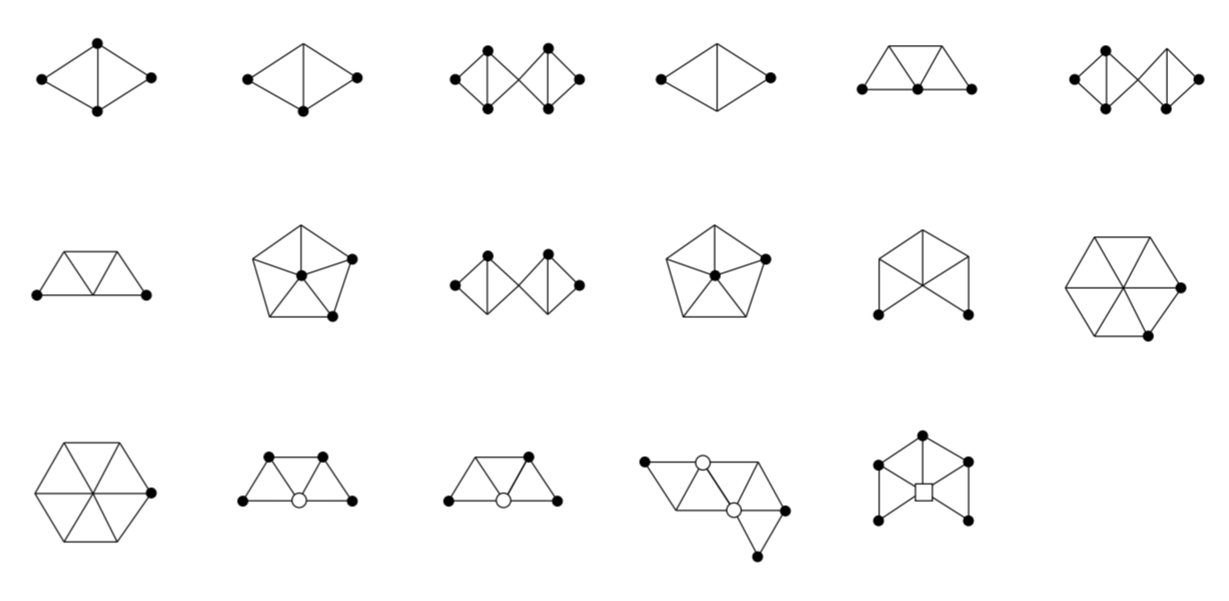
\includegraphics[width=\textwidth]{Immagine1.jpg}
    	\caption{Alcune tra le 633 configurazioni di Robertson et al.}
    	\label{fig:configurazioni}
    \end{figure}
   
    \begin{dfn}
    	Data una triangolazione $T$, si dice che $T$ {\bfseries contiene} una configurazione $K$ se $G(K)$ è un sottografo di $T$, ogni faccia finita di $G(K)$ è una faccia di $T$ e $\gamma_K(v) = \deg_T(v)$ per ogni vertice $v \in V(G(K))$.
    \end{dfn}
    Ricordiamo gli enunciati dei Teoremi 2 e 3 alla luce delle definizioni sovrastanti.
    \vspace{0.5cm}
    \\{\bfseries Teorema 2.} Nessun minimo controesempio contiene una \emph{buona configurazione}.
    \\{\bfseries Teorema 3.} Ogni \emph{triangolazione 6-connessa internamente} contiene una \emph{buona configurazione}.
    \vspace{0.5cm}
    \\La dimostrazione del Teorema 2 richiede necessariamente l'uso del computer, mentre quella del Teorema 3 potrebbe essere verificata interamente a mano, ma richiederebbe mesi di lavoro, perciò sono entrambe affidate al programma ideato da Robertson et al.
    \\Tuttavia, nelle sezioni 5.3 e 5.4 discuteremo rispettivamente il Teorema 2 e il Teorema 3 e cercheremo di capire quantomeno come si sviluppano le due dimostrazioni.
    
    \section{Riducibilità}
    Per dimostrare il Teorema 2, introduciamo il concetto di riducibilità.
    \\Si dimostra che ciascuna delle 633 configurazioni di Robertson et al. (e quindi ogni buona configurazione) è riducibile, può essere quindi sostituita con un grafo più piccolo e di conseguenza non può essere contenuta in un minimo controesempio.
    \\Per chiarire le tipologie di riducibilità di una configurazione, è necessario definire il \emph{completamento libero} di una configurazione.
    \begin{dfn}
    	Sia $K$ una configurazione. Una quasi-triangolazione $S$ si dice {\bfseries completamento libero} (\emph{free completion}) di $K$ {\bfseries con anello} $R$ se:
    	\begin{itemize}
    		\item $R$ è un ciclo di $S$ e delimita la faccia illimitata di $S$
    		\item $G(K)$ è un sottografo di S e $G(K) = S \smallsetminus V(R)$
    		\item ogni vertice $v \in S \smallsetminus V(R)$ ha $\deg_S(v) = \gamma_K(v)$.
    	\end{itemize}
    \end{dfn}
    \begin{namedthm*}{Lemma 5.2}
    	Ogni configurazione possiede un completamento libero.
    \end{namedthm*}
    \begin{proof}
    	Per generare un completamento libero $S$ di una configurazione $K$ procediamo come segue.
    	\\I vertici di $G(K)$ saranno interni a $S$, quindi non adiacenti alla faccia illimitata di $S$ e interamente circondati dall'anello $R$.
    	\\Costruiamo l'anello $R$ con questo metodo, considerando che deve valere $\deg_S(v) = \gamma_K(v)$:
    	\begin{itemize}
    		\item I vertici interni in $K$ hanno per definizione $\gamma_K(v) = \deg_K(v)$, quindi rimangono invariati.
    		\item I vertici esterni (adiacenti alla faccia illimitata) e che non siano separatori, cioè tali che $G(K) \smallsetminus v$ sia connesso, diventeranno interni in $S$, perciò dovranno avere $\deg_S(v) = \gamma_K(v)$.
    		\\Considerando che per essi vale $\gamma_K(v) > \deg_K(v)$, sarà necessario aggiungere, per ogni $v$, un numero di archi tra esso e vertici di $R$ pari a $\Delta_v = \gamma_K(v) - \deg_K(v)$.
    		\\Chiamando i vertici esterni di $K$ $v_1, \dots, v_n$ (ordinati ad esempio in senso orario), avremo che ogni coppia di archi consecutivi $(v_1, v_2), \dots, , (v_{n-1}, v_n), (v_n, v_1)$ sarà adiacente a un vertice di $R$ in comune, perciò il numero totale di vertici di $R$ sarà $\lvert R \rvert = \sum_{v \in \mathcal{V}} (\Delta_v) - n = \sum_{v \in \mathcal{V}} (\gamma_K(v) - \deg(v) - 1)$, poiché $n = \lvert \mathcal{V} \rvert$, dove $\mathcal{V} = \{v \in V(G(K)) : \text{v è adiacente alla faccia illimitata di $K$ e } G(K) \smallsetminus v \text{ è connesso}\}$.
    		\\Perciò $\lvert R \rvert$ è proprio la \emph{dimensione d'anello} citata nella definizione di configurazione.
    		\item Nel caso di vertici separatori, essi saranno sicuramente esterni in $K$ e avranno $\gamma_K(v) = \deg_K(v) + 2$.
    		\\Sarà sufficiente congiungere ciascuno di essi ai due vertici di $R$ adiacenti a entrambe le componenti connesse di $G(K) \smallsetminus v$, come nella figura esplicativa sottostante. 
    	\end{itemize}
    	La quasi-triangolazione $S$ generata con l'aggiunta di $R$ all'esterno di $G(K)$ e degli archi tra di essi è un completamento libero di $K$.
    \end{proof}
    
    \begin{figure}[H]
    	\centering
    	\begin{tikzpicture}
    		\node[circle, draw, fill=black] (a) at (0,0) {};
    		\node[circle, draw, fill=black] (b) at (1,1) {};
    		\node[circle, draw, fill=black] (c) at (1,-1) {};
    		\node[circle, draw, fill=black] (d) at (3,1) {};
    		\node[circle, draw, fill=black] (e) at (4,0) {};
    		\node[circle, draw, fill=black] (f) at (3,-1) {};
    		\node[circle, draw, minimum size=0.15cm, inner sep=0pt, fill=black] (g) at (2,0) {};
    		
    		\draw (b) -- (c) -- (a) -- (b) -- (f) -- (e) -- (d) -- (f);
    		\draw (c) -- (d);
    		
    		\draw[->, thick] (5,0) -- (7,0);
    		
    		\node[circle, draw, fill=black] (a') at (9,0) {};
    		\node[circle, draw, fill=black] (b') at (10,1) {};
    		\node[circle, draw, fill=black] (c') at (10,-1) {};
    		\node[circle, draw, fill=black] (d') at (12,1) {};
    		\node[circle, draw, fill=black] (e') at (13,0) {};
    		\node[circle, draw, fill=black] (f') at (12,-1) {};
    		\node[circle, draw, minimum size=0.15cm, inner sep=0pt, fill=black] (g') at (11,0) {};
    		
    		\node[circle, draw, fill=red] (A) at (8,0) {};
    		\node[circle, draw, fill=red] (B) at (9,2) {};
    		\node[circle, draw, fill=red] (C) at (11,2) {};
    		\node[circle, draw, fill=red] (D) at (13,2) {};
    		\node[circle, draw, fill=red] (E) at (14,0) {};
    		\node[circle, draw, fill=red] (F) at (13,-2) {};
    		\node[circle, draw, fill=red] (G) at (11,-2) {};
    		\node[circle, draw, fill=red] (H) at (9,-2) {};
    		
    		\draw (b') -- (c') -- (a') -- (b') -- (f') -- (e') -- (d') -- (f');
    		\draw (c') -- (d');
    		\draw[red, thick] (A) -- (B) -- (C) -- (D) -- (E) -- (F) -- (G) -- (H) -- (A);
    		\draw (A) -- (a') -- (B) -- (b') -- (C) -- (d') -- (D) -- (e') -- (E);
    		\draw (e') -- (F) -- (f') -- (G) -- (c') -- (H) -- (a');
    		\draw (C) -- (G);
    	\end{tikzpicture}
    	\vspace{0.5cm}
    	\caption{Consideriamo ad esempio la configurazione numero 3 della Figura~\ref{fig:configurazioni}: il vertice centrale separatore ha $\deg_K(v) = 4$ e di conseguenza $\gamma_K(v) = 6$, tutti gli altri vertici hanno $\gamma_K(v) = 5$.
    		\\Costruiamo il completamento libero di $K$ in modo da aggiungere 3 archi incidenti ai vertici di destra e sinistra, poiché essi hanno $\deg_K = 2$, e 2 archi incidenti a tutti gli altri vertici, che hanno $\deg_K = 3$. 
    		\\Per il vertice separatore centrale $v$ è sufficiente aggiungere due archi incidenti ai due vertici di $R$ adiacenti a entrambe le componenti connesse di $G(K) \smallsetminus v$, già presenti.
    		\\L'anello $R$ così generato è rappresentato in rosso.}
    \end{figure}
    \noindent Ogni completamento libero di una configurazione è sostanzialmente unico, poiché due completamenti liberi di una stessa configurazione $K$ sono legati da un isomorfismo di grafi.
    \\Infatti, dati due completamenti liberi $S$ ed $S'$ di una configurazione $K$:
    \begin{itemize}
    	\item la configurazione $K$ è fissa
    	\item la lunghezza degli anelli $R$ ed $R'$ è determinata dalla dimensione d'anello, che dipende unicamente dalla configurazione, ed è quindi la stessa in entrambi i casi
    	\item il numero di archi tra ogni vertice esterno $v$ di $K$ e quelli di $R$ è determinato da $\deg_K(v)$ e $\gamma_K(v)$, quindi dipende unicamente dalla configurazione.
    \end{itemize}
    Di conseguenza, esiste un isomorfismo $\phi \colon V(S) \to V(S')$ tale che:
    \begin{itemize}
    	\item per ogni vertice $v \in V(K)$, $\phi(v) = v$
    	\item per ogni vertice $r \in V(R)$ esiste $r' \in V(R')$ tale che $\phi(r) = r'$
    	\item $(v,r) \in E(S)$, con $v \in V(K)$ e $r \in V(R)$ $\iff (v,r') = (\phi(v), \phi(r)) \in E(S')$.
    \end{itemize}
    \vspace{0.5cm}
    Dato un ciclo $R$, esiste una proprietà di \emph{consistenza (consistency)} di un insieme di 4-colorazioni di $R$ che è stato utilizzato da Kempe e Birkhoff.
    \\Per i nostri scopi, non è necessario definire cosa si intenda per \emph{consistenza}, ma è sufficiente enunciare le seguenti proprietà:
    \begin{enumerate}
    	\item  l'insieme vuoto è consistente
    	\item l'unione di due insiemi consistenti è consistente
    	\item se $T$ è una triangolazione, $R$ è un ciclo di $T$, $T'$ è la quasi-triangolazione ottenuta rimuovendo da $T$ tutti i vertici interni al disco aperto delimitato da $R$ e $\mathcal{C}$ è l'insieme di tutte le restrizioni delle 4-colorazioni di $T'$ a $R$, allora $\mathcal{C}$ è consistente
    	\item la consistenza è una proprietà abbastanza restrittiva da permettere l'esistenza di abbastanza \emph{configurazioni riducibili} (ne chiariremo il significato in seguito).
    \end{enumerate}
    Dato un completamento libero $S$ di una configurazione $K$ con anello $R$, sia $\mathcal{C}^*$ l'insieme di tutte le 4-colorazioni di $R$ e sia $\mathcal{C}$ l'insieme di tutte le restrizioni a $V(R)$ delle 4-colorazioni di $S$ (si dimostra facilmente che ognuna delle 633 configurazioni di Robertson et al., che sono le uniche che saranno utili nel seguito, sono 4-colorabili, come anche i loro completamenti liberi).
    \\Sia inoltre $\mathcal{C}'$ il sottoinsieme consistente massimale di $\mathcal{C}^* \smallsetminus \mathcal{C}$.
    \\Diamo due diverse definizioni di \emph{riducibilità} della configurazione $K$.
    \begin{dfn}
    	La configurazione $K$ si dice {\bfseries $\mathit{D}$-riducibile} se $\mathcal{C}' = \emptyset$.
    \end{dfn}
    \begin{dfn}
    	La configurazione $K$ si dice {\bfseries $\mathit{C}$-riducibile} se esiste una quasi-triangolazione $S'$, chiamata {\bfseries riduttrice}, ottenuta da $S$ sostituendo $G(K)$ con un grafo più piccolo, in modo che nessun elemento di $\mathcal{C}'$ sia la restrizione a $V(R)$ di una 4-colorazione di $S'$.
    \end{dfn}
    Per giungere alla dimostrazione del Teorema 2, vogliamo provare che nessun minimo controesempio al Teorema dei Quattro colori può contenere una configurazione $\mathit{D}$-riducibile o $\mathit{C}$-riducibile.
    \\Per quanto riguarda la $\mathit{D}$-riducibilità, la dimostrazione non presenta particolari problemi, come vedremo in seguito. Per quanto riguarda invece la $\mathit{C}$-riducibilità, che sembra essere la definizione più "naturale" di riducibilità, la dimostrazione è in realtà molto più problematica, poiché porterebbe a una sostituzione di $S$ con $S'$, tuttavia non abbiamo la certezza che $S'$ sia privo di cappi, e quindi semplice.
    \\A tale scopo, consideriamo soltanto riduttrici \emph{sicure}.
    \begin{dfn}
    	Una riduttrice si dice {\bfseries sicura} se il processo di sostituzione sopraccitato, a partire da una triangolazione $T$ 6-connessa internamente, produce una triangolazione.
    \end{dfn}
    \begin{namedthm*}{Lemma 5.3}
    	Un minimo controesempio al Teorema dei Quattro Colori non può contenere configurazioni $\mathit{D}$-riducibili oppure $\mathit{C}$-riducibili con una riduttrice sicura.
    \end{namedthm*}
    \begin{proof}[Dimostrazione (accenno)]
    	Per quanto riguarda la prima parte del Lemma, qualora un minimo controesempio $G$ contenesse una configurazione $\mathit{D}$-riducibile $K$, avremmo $\mathcal{C}' = \emptyset$.
    	\\Di conseguenza, dato un completamento libero $S$ di $K$ con anello $R$, l'insieme delle 4-colorazioni di $R$, considerato autonomo rispetto ad $S$, e l'insieme delle 4-colorazioni di $R$, come restrizioni delle 4-colorazioni di $S$, sono sostanzialmente uguali tra loro, nel senso che la differenza tra i due insiemi ha sottoinsieme consistente massimale vuoto.
    	\\Perciò, la presenza di $G(K)$ non influisce sulla 4-colorabilità dei vertici di $R$ e, in generale, di ogni vertice adiacente a $G(K)$ (non è infatti necessariamente vero che tutto $R$ sia contenuto in $G$).
    	\\$G(K)$ potrebbe allora essere sostituito ad esempio da un grafo vuoto ed $R$ avrebbe sostanzialmente lo stesso insieme di 4-colorazioni possibili.
    	\\Se $G$ contiene una configurazione $\mathit{D}$-riducibile, non può essere un minimo controesempio al Teorema dei Quattro Colori.
    	\\Consideriamo un esempio semplice in cui non soltanto $\mathcal{C}' = \emptyset$, ma $\mathcal{C}^* \smallsetminus \mathcal{C} = \emptyset$, quindi non è necessaria una reale comprensione del concetto di consistenza.
    	\begin{figure}[H]
    		\centering
    		\resizebox{\textwidth}{!}{
    		\begin{tikzpicture}
    			\node[draw, circle, fill=black] (a) at (0,0) {};
    			\node[draw, circle, fill=black] (b) at (1,1.5) {};
    			\node[draw, circle, fill=black] (c) at (3,1.5) {};
    			\node[draw, circle, fill=black] (d) at (4,0) {};
    			\node[draw, circle, fill=black] (e) at (3,-1.5) {};
    			\node[draw, circle, fill=black] (f) at (1,-1.5) {};
    			\node[circle, draw, minimum size=0.15cm, inner sep=0pt, fill=black] (g) at (2,0) {};
    			\node[circle, draw, minimum size=0.15cm, inner sep=0pt, fill=black] (h) at (2,3) {};
    			\node[draw, circle, fill=black] (i) at (5,1.5) {};
    			\node[circle, draw, minimum size=0.15cm, inner sep=0pt, fill=black] (j) at (5,-1.5) {};
    			\node[draw, circle, fill=black] (k) at (2,-3) {};
    			\node[circle, draw, minimum size=0.15cm, inner sep=0pt, fill=black] (l) at (-1,-1.5) {};
    			\node[draw, circle, fill=black] (m) at (-1,1.5) {};
    			
    			\node[draw, circle, fill=red] (p) at (2,-6) {};
    			\node[draw, circle, fill=red] (n) at (-4,3) {};
    			\node[draw, circle, fill=red] (o) at (8,3) {};
    			
    			\draw (h) -- (j) -- (l) -- (h) -- (i) -- (k) -- (m) -- (i) -- (j) -- (k) -- (l) -- (m) -- (h);
    			\draw (a) -- (d);
    			\draw (b) -- (e);
    			\draw (c) -- (f);
    			
    			\draw (m) -- (n) -- (o) -- (p) -- (n);
    			\draw (i) -- (o);
    			\draw (k) -- (p);
    			\draw[red, thick] (n) .. controls (2,5) .. (o) .. controls (6.66,-2.61) .. (p) .. controls (-2.66,-2.61) .. (n);
    			
    			\draw[->, thick] (9,-0.5) -- (11,-0.5);
    			
    			\node[draw, circle, fill=green] (a) at (16,0) {};
    			\node[draw, circle, fill=red] (b) at (17,1.5) {};
    			\node[draw, circle, fill=blue] (c) at (19,1.5) {};
    			\node[draw, circle, fill=green] (d) at (20,0) {};
    			\node[draw, circle, fill=blue] (e) at (19,-1.5) {};
    			\node[draw, circle, fill=red] (f) at (17,-1.5) {};
    			\node[circle, draw, fill=yellow] (g) at (18,0) {};
    			\node[circle, draw, fill=green] (h) at (18,3) {};
    			\node[draw, circle, fill=yellow] (i) at (21,1.5) {};
    			\node[circle, draw, fill=red] (j) at (21,-1.5) {};
    			\node[draw, circle, fill=yellow] (k) at (18,-3) {};
    			\node[circle, draw, fill=blue] (l) at (15,-1.5) {};
    			\node[draw, circle, fill=yellow] (m) at (15,1.5) {};
    			
    			\node[draw, circle, fill=green] (p) at (18,-6) {};
    			\node[draw, circle, fill=red] (n) at (12,3) {};
    			\node[draw, circle, fill=blue] (o) at (24,3) {};
    			
    			\draw (h) -- (c) -- (d) -- (j) -- (e) -- (f) -- (l) -- (a) -- (b) -- (h) -- (i) -- (d) -- (e) -- (k) -- (f) -- (a) -- (m) -- (b) -- (c) -- (i) -- (j) -- (k) -- (l) -- (m) -- (h);
    			\draw (a) -- (g) -- (d);
    			\draw (b) -- (g) -- (e);
    			\draw (c) -- (g) -- (f);
    			
    			\draw (m) -- (n) -- (h) -- (o) -- (j) -- (p) -- (l) -- (n);
    			\draw (i) -- (o);
    			\draw (k) -- (p);
    			\draw[red, thick] (n) .. controls (18,5) .. (o) .. controls (22.66,-2.61) .. (p) .. controls (13.34,-2.61) .. (n);
    		\end{tikzpicture}
    	}
    	\vspace{0.5cm}
    	\caption{Un esempio di configurazione $\mathit{D}$-riducibile.}
    	\end{figure} 
    	\noindent Nella parte sinistra dell'esempio in figura sono rappresentati una configurazione $K$ (in nero) con la convenzione di Heesch e il suo completamento libero $S$ con anello $R$ (in rosso).
    	\\Ogni 4-colorazione di $R$ è individuata semplicemente dall'utilizzo di 3 colori diversi per i 3 vertici (rosso, blu e verde in questo caso) e ognuna di queste colorazioni è anche restrizione di una 4-colorazione di $S$ e sostanzialmente unica a meno di scambi di colori, come si può vedere ad esempio nella figura di destra.
    	\\Di conseguenza, in questo caso $\mathcal{C}' = \mathcal{C}^* \smallsetminus \mathcal{C} = \emptyset$, quindi $K$ è $\mathit{D}$-riducibile e potrebbe essere sostituita semplicemente da un grafo vuoto.
    	\\\emph{Nota:} $S$ non può in realtà comparire in un eventuale controesempio minimo $G$ già per ipotesi, poiché $R$ sarebbe un ciclo separatore di lunghezza 3 e di conseguenza $G$ non sarebbe 6-connesso internamente.
    	\vspace{0.5cm}
    	
    	Per quanto riguarda la seconda parte, per definizione di $\mathit{C}$-riducibilità, la presenza di una configurazione $\mathit{C}$-riducibile in un minimo controesempio (se con riduttrice sicura) è impossibile, perché permetterebbe la sostituzione di $G(K)$ con un grafo più piccolo.
    	\\L'unica difficoltà è quindi la dimostrazione della \emph{sicurezza}, affidata al programma elaborato da Robertson et al. e molto meno problematica rispetto a quanto lo sia nella dimostrazione di Appel e Haken.
    	\\In questo caso vengono infatti considerate soltanto riduttrici ottenute da $G(K)$ tramite contrazione di 4 archi al massimo, rendendo la verifica della \emph{sicurezza} più semplice.
    	
    	Consideriamo anche in questo caso un semplice esempio esplicativo di configurazione $\mathit{C}$-riducibile: la prima configurazione della Figura~\ref{fig:configurazioni}, che chiameremo $C_1$, il cui completamento libero viene chiamato \emph{diamante di Birkhoff} {\bfseries \cite{Steinberger}}.
    	\begin{figure}[H]
    		\centering
    		\begin{tikzpicture}
    		\node[draw, circle, minimum size=0.6cm, inner sep=0pt] (a) at (0,0) {$u_1$};	
    		\node[draw, circle, minimum size=0.6cm, inner sep=0pt] (b) at (1,0.67) {$u_2$};
    		\node[draw, circle, minimum size=0.6cm, inner sep=0pt] (c) at (2,0) {$u_3$};
    		\node[draw, circle, minimum size=0.6cm, inner sep=0pt] (d) at (1,-0.67) {$u_4$};
    		
    		\node[draw=red, circle, minimum size=0.6cm, inner sep=0pt] (e) at (0,1.33) {$v_1$};
    		\node[draw=red, circle, minimum size=0.6cm, inner sep=0pt] (f) at (2,1.33) {$v_2$};
    		\node[draw=red, circle, minimum size=0.6cm, inner sep=0pt] (g) at (3,0) {$v_3$};
    		\node[draw=red, circle, minimum size=0.6cm, inner sep=0pt] (h) at (2,-1.33) {$v_4$};
    		\node[draw=red, circle, minimum size=0.6cm, inner sep=0pt] (i) at (0,-1.33) {$v_5$};
    		\node[draw=red, circle, minimum size=0.6cm, inner sep=0pt] (j) at (-1,0) {$v_6$};
    		
    		\draw (j) -- (a) -- (e) -- (b) -- (d) -- (a) -- (b) -- (c) -- (d) -- (i) -- (a);
    		\draw (b) -- (f) -- (c) -- (g);
    		\draw (c) -- (h) -- (d);
    		
    		\draw[red] (e) -- (f) -- (g) -- (h) -- (i) -- (j) -- (e);
    		
    		\draw[->, thick] (4,0) -- (6,0);
    		
    		\node[draw=red, circle, minimum size=0.6cm, inner sep=0pt] (E) at (8,1.33) {$v_1$};
    		\node[draw=red, circle, minimum size=0.6cm, inner sep=0pt] (F) at (9.5,0) {$v$};
    		\node[draw=red, circle, minimum size=0.6cm, inner sep=0pt] (G) at (11,0) {$v_3$};
    		\node[draw=red, circle, minimum size=0.6cm, inner sep=0pt] (H) at (8,-1.33) {$v_5$};
    		\node[draw=red, circle, minimum size=0.6cm, inner sep=0pt] (I) at (7,0) {$v_6$};
    		
    		\draw[red] (G) -- (F) -- (I) -- (E) -- (F) -- (H) -- (I);
    		\end{tikzpicture}
    		\vspace{0.5cm}
    		\caption{Contrazione del diamante di Birkhoff}
    	\end{figure}
    	Il diamante di Birkhoff $S$ rappresentato nella parte sinistra della figura, completamento libero di $C_1$, può essere ridotto tramite contrazione al grafo $S' = S/\{u_1, u_2, u_3, u_4, v_2, v_4\}$, rappresentato a destra, in cui $v$ è la contrazione dei 6 vertici.
    	\\Dimostriamo che ogni 4-colorazione di $S'$ può essere estesa anche ad $S$, che di conseguenza non può essere presente in un minimo controesempio {\bfseries \cite{Nanjwenge}}.
    	\\Consideriamo tutte le 4-colorazioni di $S'$, che sono 6: fissiamo 3 colori, diversi tra loro, per $v$, $v_1$ e $v_6$, ad esempio blu, rosso e verde rispettivamente. Così facendo rimangono 2 colori disponibili per $v_5$, ovvero rosso e giallo, e 3 colori per $v_3$, ovvero rosso, verde e giallo, quindi il numero di scelte totali è 6.
    	\\Applichiamo ciascuna di queste 6 colorazioni all'anello $R$ di $S$ (rappresentato in rosso) utilizzando per $v_2$ e $v_4$ lo stesso colore di $v$, in questo caso il blu, e mostriamo le 6 colorazioni di $S$ che si ottengono.
    	\\Le prime 5 colorazioni si ottengono in modo molto semplice a partire dalla rispettiva colorazione di $R$, mentre la colorazione 6 richiede l'utilizzo delle catene di Kempe per rendere possibile la colorazione di $C_1$.
    	\begin{figure}[H]
    		\centering
    		\begin{subfigure}{0.3\textwidth}
    			\centering
    			\begin{tikzpicture}
    				\node[draw, circle, fill=blue] (a) at (0,0) {};	
    				\node[draw, circle, fill=green] (b) at (1,0.67) {};
    				\node[draw, circle, fill=yellow] (c) at (2,0) {};
    				\node[draw, circle, fill=red] (d) at (1,-0.67) {};
    				
    				\node[draw, circle, fill=red] (e) at (0,1.33) {};
    				\node[draw, circle, fill=blue] (f) at (2,1.33) {};
    				\node[draw, circle, fill=green] (g) at (3,0) {};
    				\node[draw, circle, fill=blue] (h) at (2,-1.33) {};
    				\node[draw, circle, fill=yellow] (i) at (0,-1.33) {};
    				\node[draw, circle, fill=green] (j) at (-1,0) {};
    				
    				\draw (j) -- (a) -- (e) -- (b) -- (d) -- (a) -- (b) -- (c) -- (d) -- (i) -- (a);
    				\draw (b) -- (f) -- (c) -- (g);
    				\draw (c) -- (h) -- (d);
    				
    				\draw[red] (e) -- (f) -- (g) -- (h) -- (i) -- (j) -- (e);
    			\end{tikzpicture}
    			\caption{Colorazione 1.}
    		\end{subfigure}
    		\begin{subfigure}{0.3\textwidth}
    			\centering
    			\begin{tikzpicture}
    				\node[draw, circle, fill=blue] (a) at (0,0) {};	
    				\node[draw, circle, fill=yellow] (b) at (1,0.67) {};
    				\node[draw, circle, fill=green] (c) at (2,0) {};
    				\node[draw, circle, fill=red] (d) at (1,-0.67) {};
    				
    				\node[draw, circle, fill=red] (e) at (0,1.33) {};
    				\node[draw, circle, fill=blue] (f) at (2,1.33) {};
    				\node[draw, circle, fill=yellow] (g) at (3,0) {};
    				\node[draw, circle, fill=blue] (h) at (2,-1.33) {};
    				\node[draw, circle, fill=yellow] (i) at (0,-1.33) {};
    				\node[draw, circle, fill=green] (j) at (-1,0) {};
    				
    				\draw (j) -- (a) -- (e) -- (b) -- (d) -- (a) -- (b) -- (c) -- (d) -- (i) -- (a);
    				\draw (b) -- (f) -- (c) -- (g);
    				\draw (c) -- (h) -- (d);
    				
    				\draw[red] (e) -- (f) -- (g) -- (h) -- (i) -- (j) -- (e);
    			\end{tikzpicture}
    			\caption{Colorazione 2.}
    		\end{subfigure}
    		\begin{subfigure}{0.3\textwidth}
    		\centering
    		\begin{tikzpicture}
    			\node[draw, circle, fill=blue] (a) at (0,0) {};	
    			\node[draw, circle, fill=yellow] (b) at (1,0.67) {};
    			\node[draw, circle, fill=green] (c) at (2,0) {};
    			\node[draw, circle, fill=red] (d) at (1,-0.67) {};
    			
    			\node[draw, circle, fill=red] (e) at (0,1.33) {};
    			\node[draw, circle, fill=blue] (f) at (2,1.33) {};
    			\node[draw, circle, fill=red] (g) at (3,0) {};
    			\node[draw, circle, fill=blue] (h) at (2,-1.33) {};
    			\node[draw, circle, fill=yellow] (i) at (0,-1.33) {};
    			\node[draw, circle, fill=green] (j) at (-1,0) {};
    			
    			\draw (j) -- (a) -- (e) -- (b) -- (d) -- (a) -- (b) -- (c) -- (d) -- (i) -- (a);
    			\draw (b) -- (f) -- (c) -- (g);
    			\draw (c) -- (h) -- (d);
    			
    			\draw[red] (e) -- (f) -- (g) -- (h) -- (i) -- (j) -- (e);
    		\end{tikzpicture}
    		\caption{Colorazione 3.}
    		\end{subfigure}
    		\begin{subfigure}{0.3\textwidth}
    		\centering
    		\begin{tikzpicture}
    			\node[draw, circle, fill=blue] (a) at (0,0) {};	
    			\node[draw, circle, fill=yellow] (b) at (1,0.67) {};
    			\node[draw, circle, fill=red] (c) at (2,0) {};
    			\node[draw, circle, fill=green] (d) at (1,-0.67) {};
    			
    			\node[draw, circle, fill=red] (e) at (0,1.33) {};
    			\node[draw, circle, fill=blue] (f) at (2,1.33) {};
    			\node[draw, circle, fill=green] (g) at (3,0) {};
    			\node[draw, circle, fill=blue] (h) at (2,-1.33) {};
    			\node[draw, circle, fill=red] (i) at (0,-1.33) {};
    			\node[draw, circle, fill=green] (j) at (-1,0) {};
    			
    			\draw (j) -- (a) -- (e) -- (b) -- (d) -- (a) -- (b) -- (c) -- (d) -- (i) -- (a);
    			\draw (b) -- (f) -- (c) -- (g);
    			\draw (c) -- (h) -- (d);
    			
    			\draw[red] (e) -- (f) -- (g) -- (h) -- (i) -- (j) -- (e);
    		\end{tikzpicture}
    		\caption{Colorazione 4.}
    		\end{subfigure}
    		\begin{subfigure}{0.3\textwidth}
    			\centering
    			\begin{tikzpicture}
    				\node[draw, circle, fill=blue] (a) at (0,0) {};	
    				\node[draw, circle, fill=yellow] (b) at (1,0.67) {};
    				\node[draw, circle, fill=red] (c) at (2,0) {};
    				\node[draw, circle, fill=green] (d) at (1,-0.67) {};
    				
    				\node[draw, circle, fill=red] (e) at (0,1.33) {};
    				\node[draw, circle, fill=blue] (f) at (2,1.33) {};
    				\node[draw, circle, fill=yellow] (g) at (3,0) {};
    				\node[draw, circle, fill=blue] (h) at (2,-1.33) {};
    				\node[draw, circle, fill=red] (i) at (0,-1.33) {};
    				\node[draw, circle, fill=green] (j) at (-1,0) {};
    				
    				\draw (j) -- (a) -- (e) -- (b) -- (d) -- (a) -- (b) -- (c) -- (d) -- (i) -- (a);
    				\draw (b) -- (f) -- (c) -- (g);
    				\draw (c) -- (h) -- (d);
    				
    				\draw[red] (e) -- (f) -- (g) -- (h) -- (i) -- (j) -- (e);
    			\end{tikzpicture}
    			\caption{Colorazione 5.}
    		\end{subfigure}
    		\begin{subfigure}{0.3\textwidth}
    			\centering
    			\begin{tikzpicture}
    				\node[draw, circle] (a) at (0,0) {};	
    				\node[draw, circle] (b) at (1,0.67) {};
    				\node[draw, circle] (c) at (2,0) {};
    				\node[draw, circle] (d) at (1,-0.67) {};
    				
    				\node[draw, circle, fill=red] (e) at (0,1.33) {};
    				\node[draw, circle, fill=blue] (f) at (2,1.33) {};
    				\node[draw, circle, fill=red] (g) at (3,0) {};
    				\node[draw, circle, fill=blue] (h) at (2,-1.33) {};
    				\node[draw, circle, fill=red] (i) at (0,-1.33) {};
    				\node[draw, circle, fill=green] (j) at (-1,0) {};
    				
    				\draw (j) -- (a) -- (e) -- (b) -- (d) -- (a) -- (b) -- (c) -- (d) -- (i) -- (a);
    				\draw (b) -- (f) -- (c) -- (g);
    				\draw (c) -- (h) -- (d);
    				
    				\draw[red] (e) -- (f) -- (g) -- (h) -- (i) -- (j) -- (e);
    			\end{tikzpicture}
    			\caption{Colorazione 6.}
    		\end{subfigure}
    		\caption{Le 6 colorazioni di $S$ ricavate a partire dalle colorazioni di $S'$.}
    		\end{figure}
    		Per quanto riguarda la colorazione 6, utilizzando i nomi assegnati ai vertici in precedenza, individuiamo la catena di Kempe rossa-gialla contenente $v_3$ e abbiamo 3 possibili casi:
    		\begin{itemize}
    			\item La catena non è ciclica né con $v_1$ né con $v_5$, gli altri due vertici rossi.
    			\\In questo caso invertiamo i colori all'interno della catena, colorando quindi $v_3$ di giallo, e ci riconduciamo alla colorazione 5.
    			\item La catena è ciclica con $v_1$ ma non con $v_5$ (o viceversa).
    			\\Individuiamo allora la catena di Kempe rossa-gialla contenente $v_5$ (rispettivamente $v_1$), ne invertiamo i colori, colorando così $v_5$ (o $v_1$) di giallo e riconducendoci quindi alla colorazione 3.
    			\item La catena è ciclica sia con $v_1$ che con $v_5$.
    			\\In quest'ultimo caso individuiamo allora la catena di Kempe blu-verde contenente $v_4$, che non può essere ciclica con il vertice verde $v_6$ per la planarità del grafo.
    			\\Invertiamo i colori all'interno della catena e coloriamo $v_4$ di verde, possiamo allora estendere la 4-colorazione anche ai vertici di $C_1$, come illustrato nella figura sottostante.
    		\end{itemize}
    		\begin{figure}[H]
    			\centering
    			\begin{tikzpicture}
    				\node[draw, circle, fill=yellow] (a) at (0,0) {};	
    				\node[draw, circle, fill=green] (b) at (1,0.67) {};
    				\node[draw, circle, fill=yellow] (c) at (2,0) {};
    				\node[draw, circle, fill=blue] (d) at (1,-0.67) {};
    				
    				\node[draw, circle, fill=red] (e) at (0,1.33) {};
    				\node[draw, circle, fill=blue] (f) at (2,1.33) {};
    				\node[draw, circle, fill=red] (g) at (3,0) {};
    				\node[draw, circle, fill=green] (h) at (2,-1.33) {};
    				\node[draw, circle, fill=red] (i) at (0,-1.33) {};
    				\node[draw, circle, fill=green] (j) at (-1,0) {};
    				
    				\draw (j) -- (a) -- (e) -- (b) -- (d) -- (a) -- (b) -- (c) -- (d) -- (i) -- (a);
    				\draw (b) -- (f) -- (c) -- (g);
    				\draw (c) -- (h) -- (d);
    				
    				\draw[red] (e) -- (f) -- (g) -- (h) -- (i) -- (j) -- (e);
    			\end{tikzpicture}
    			\caption{Colorazione 6.}
    		\end{figure}
    		La configurazione $C_1$ è quindi $\mathit{C}$-riducibile, può essere sostituita da un grafo più piccolo e di conseguenza non può essere contenuta in un minimo controesempio al Teorema dei Quattro Colori. 
    \end{proof}
    
    A questo punto, per dimostrare il Teorema 2, è sufficiente provare il seguente Lemma.
    \begin{namedthm*}{Lemma 5.4}
    	Ciascuna delle 633 configurazioni di Robertson et al. è $\mathit{D}$-riducibile o $\mathit{C}$-riducibile con una riduttrice sicura.
    \end{namedthm*}
    \noindent La dimostrazione del Lemma 5.4 non può essere eseguita a mano, ed è infatti affidata a due programmi indipendenti, elaborati da Robertson et al., che individuano anche una serie di invarianti numerici da poter confrontare per consentire una verifica della correttezza dei risultati.
    \\La dimostrazione del Lemma 5.3 e del Lemma 5.4 prova che nessuna delle 633 configurazioni (e di conseguenza nessuna buona configurazione) può essere contenuta in un minimo controesempio al Teorema dei Quattro Colori, perciò anche il Teorema 2 è dimostrato.
   
    \section{Inevitabilità}
    Il Teorema 3, che dimostreremo in questa sezione, afferma l'\emph{inevitabilità} della presenza di una buona configurazione in ogni triangolazione 6-connessa internamente.
    \begin{dfn}
    	Una configurazione $K$ {\bfseries compare} in una configurazione $L$ se $G(K)$ è un sottografo di $G(L)$, ogni faccia finita di $K$ è una faccia finita di $L$ e $\gamma_K(v) = \gamma_L(v)$ per ogni $v \in V(K)$.
    \end{dfn}
    \begin{dfn}
    	Sia $T$ una triangolazione 6-connessa internamente.
    	\\Dato un vertice $v$ di $T$, si dice {\bfseries vicinato} di $v$ in $T$ la configurazione $K$ tale che $G(K)$ sia il sottografo di $T$ indotto da tutti i vertici $u$ di $T$ per i quali esiste un cammino $P$ in $T$ con estremi $u$ e $v$ e lunghezza massima 2, in cui il vertice centrale (se presente) ha grado massimo 8, e $\gamma_K(u) = \deg_T(u)$ per ogni $u \in V(K)$.    	
    \end{dfn}
    Per dimostrare il Teorema 3, proviamo che una buona configurazione compare necessariamente nel vicinato di un certo vertice.
    \begin{dfn}
    	Dato un grafo planare $G$, una {\bfseries regola} (\emph{di scarica}) è una 6-upla $(G, \alpha, \epsilon, r, s, t)$, in cui 
    	\\$\alpha \colon V(G) \to \{5, 6, 7, 8\}$ ed $\epsilon \colon V(G) \to \{-, 0, +\}$ sono applicazioni, $r > 0$ è un numero intero, $s$ e $t$ sono due vertici adiacenti di $G$.
    \end{dfn}
    La Figura~\ref{fig:regole} rappresenta l'insieme $\mathcal{R}$ di tutte le 32 \emph{regole} di Robertson et al. seguendo la convenzione seguente:
    \begin{itemize}
    	\item  l'applicazione $\alpha$ segue la convenzione di Heesch introdotta per le 633 configurazioni (cerchio pieno $\bullet$ se $\alpha(v) = 5$, punto $\cdot$ se $\alpha(v) = 6$, cerchio vuoto $\circ$ se $\alpha(v) = 7$, quadrato vuoto $\square$ se $\alpha(v) = 8$)
    	\item $\epsilon$ corrisponde al \emph{segno} del vertice ed è rappresentata con il segno + o - di fianco al vertice corrispondente (il segno 0 è omesso)
    	\item $s, t \in V(G)$ sono tali che l'unico arco direzionato rappresentato sia da $s$ a $t$
    	\item $r$ è il numero di frecce rappresentate sull'arco $(s, t)$, \\$r = 2$ per la prima regola ed $r = 1$ per le 31 regole restanti.
    \end{itemize}
    Le prime 7 regole seguono una sorta di "pattern", ma tutte le regole restanti sono state individuate da Robertson et al. tramite un metodo per tentativi.
    \begin{dfn}
    Un {\bfseries passaggio} (\emph{di carica}) $P$ è una 4-upla $(K, r, s, t)$, in cui $K$ è una configurazione, $r > 0$ è un numero intero ed $s, t \in V(K)$ sono tali che esistono una regola $R = (G, \alpha, \epsilon, r, s', t') \in \mathcal{R}$ e un isomorfismo di grafi $h \colon G(K) \to G$ con le seguenti proprietà:
    \begin{enumerate}
    	\item $\gamma_K(v) \leq \alpha(h(v))$ per ogni $v \in V(K)$ con $\epsilon(h(v)) \in \{-,0\}$
    	\item $\gamma_K(v) \geq \alpha(h(v))$ per ogni $v \in V(K)$ con $\epsilon(h(v))\in \{0,+\}$
    	\item $h(s) = s'$ e $h(t) = t'$.
    \end{enumerate}
    Diciamo che $P$ {\bfseries rispetta} la regola $R$, ogni passaggio rispetta esattamente un'unica regola.
    \\Scriveremo $r(P) = r$, $s(P) = s$, $t(P) = t$.
    \\$r$ è il \emph{valore} del passaggio, $s$ la sua \emph{sorgente} e $t$ il suo \emph{pozzo}.
    \\Un passaggio $P$ è \emph{contenuto} in una triangolazione $T$ o in una configurazione $L$ se $K(P)$ è contenuta in $T$ o $L$. 
    \end{dfn}
    Una volta definita nel seguito la \emph{carica} di un vertice, il significato di passaggio sarà esattamente quello di un passaggio di carica tra i vertici $s$ e $t$ seguendo una delle 32 regole.
    \\In particolare, nell'algoritmo presentato da Robertson et al., i passaggi di carica saranno fondamentali per individuare una delle 633 configurazioni, seguendo lo spostamento delle cariche all'interno del grafo.
    \begin{figure}[H]
    	\centering
    	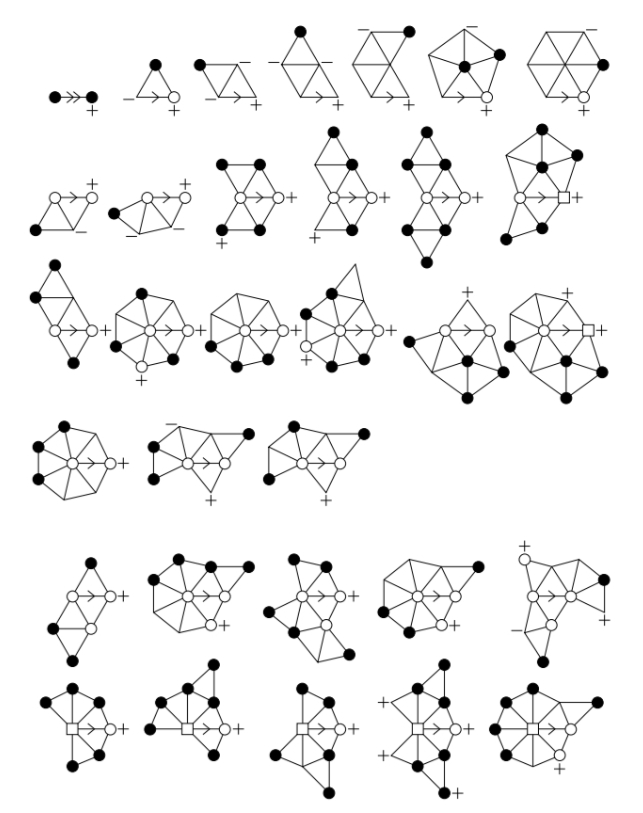
\includegraphics[width=\textwidth, height=20cm]{Immagine2.jpg}
    	\caption{Le 32 regole di Robertson et al.}
    	\label{fig:regole}
    \end{figure}
    
    Definiamo ora la \emph{carica} di un vertice.
    \begin{dfn}
    	Dato un vertice $v$ di una triangolazione $T$, definiamo la sua {\bfseries carica} come
    	\[
    	 \Theta_T(v) = 10(6 - \deg_T(v)) + \sum_{\substack{P \text{ contenuti in } T \\ t(P) = v}} r(P) - \sum_{\substack{P \text{ contenuti in } T \\ s(P) = v}} r(P)
    	\]
    	dove tutti i $P$ sono passaggi.
        \\La carica $\Theta_T(v)$ dipende soltanto dal vicinato di $v$ in $T$, poiché nel primo termine $\deg_T(v)$ dipende dai vertici adiacenti a $v$, che fanno parte del suo vicinato, e il secondo e terzo termine dipendono dai passaggi in cui $v$ è pozzo o sorgente. Ogni passaggio fa interamente parte del vicinato del proprio pozzo e della propria sorgente, come è facile verificare direttamente dall'elenco delle 32 regole presentate nella Figura~\ref{fig:regole}.
    \end{dfn}
    \begin{namedthm*}{Lemma 5.5}
    	Per ogni triangolazione $T$, $\sum_{v \in V(T)} \Theta_T(v) = 120$.
    	\\Perciò, esiste un vertice $v$ di $T$ tale che $\Theta_T(v) > 0$.
    \end{namedthm*}
    \begin{proof}
    	Nelle sommatorie $V$ sta per $V(T)$ e per $P$ si intendono tutti i passi $P$ contenuti in $T$.
    	\[
    	\sum_{v \in V} \Theta_T(v) = \sum_{v \in V} \Big[ 10(6 - \deg_T(v)) + \sum_{P} r(P) \cdot \delta_{t(P), v} - \sum_{P} r(P) \cdot \delta_{s(P), v} \Big],
    	\]
    	dove $\delta_{t(P), v}$ e $\delta_{s(P), v}$ sono funzioni indicatrici che valgono $1$ se $t(P) = v$ o $s(P) = v$, rispettivamente, e $0$ altrimenti.
    	\\Per linearità, possiamo calcolare la sommatoria sui tre termini separatamente:
    	\[
    	\sum_{v \in V} \Theta_T(v) = \sum_{v \in V} 10(6 - \deg_T(v)) + \sum_{v \in V} \sum_{P} r(P) \cdot \delta_{t(P), v} - \sum_{v \in V} \sum_{P} r(P) \cdot \delta_{s(P), v}.
    	\]
    	Consideriamo singolarmente il primo termine: $\sum_{v \in V} 10(6 - \deg_T(v))$.
    	\\Come per ogni grafo, anche $T$ soddisfa:
    	\[
    	\sum_{v \in V} \deg_T(v) = 2\lvert E \rvert,
     	\]
    	dove $E = E(T)$ è l'insieme degli archi di T. 
    	\\Inoltre, poiché $T$ è una triangolazione, e quindi un grafo planare massimale, sappiamo che:
    	\[
    	\lvert E \rvert = 3\lvert V \rvert - 6.
    	\]
    	Quindi:
    	\[
    	\sum_{v \in V} \deg_T(v) = 2(3\lvert V \rvert - 6) = 6\lvert V \rvert - 12.
    	\]
    	Pertanto avremo che
    	\[
    	\sum_{v \in V} 10(6 - \deg_T(v)) = 10 \Big(6\lvert V \rvert - \sum_{v \in V} \deg_T(v)\Big) = 10 \Big(6\lvert V \rvert - (6\lvert V \rvert - 12)\Big) = 10 \cdot 12 = 120.
    	\]
    	
    	Per quanto riguarda invece secondo e terzo termine, è sufficiente notare che se $P$ è un passo contenuto in $T$, allora esisteranno necessariamente sia un vertice $u \in V(T)$ tale che $t(P) = u$, sia un vertice $v \in V(T)$ tale che $s(P) = v$.
    	\\Sommando quindi su tutti i vertici in $V(T)$ i due termini si cancellano:
    	\[
    	\sum_{v \in V} \sum_{P} r(P) \cdot \delta_{t(P), v} - \sum_{v \in V} \sum_{P} r(P) \cdot \delta_{s(P), v} = 0.
    	\]
    	
    	Quindi risulta
    	\[
    	\sum_{v \in V} \Theta_T(v) = 120 + 0 = 120.
    	\]
    	Perciò, la somma totale delle cariche dei vertici in una triangolazione $T$ è pari a $120$ e di conseguenza esiste almeno un vertice $v$ di $T$ tale che $\Theta_T(v) > 0$.
    \end{proof}
    A questo punto, per dimostrare il Teorema 3 è sufficiente dimostrare invece il Teorema seguente.
    \begin{namedthm*}{Teorema 4}
    	Se $v$ è un vertice di una triangolazione $T$ 6-connessa internamente con $\Theta_T(v) > 0$, allora è presente una buona configurazione contenuta in $T$ nel vicinato di $v$.
    \end{namedthm*}
    Chiamiamo $C_1, C_2, \dots, C_{17}$ le 17 configurazioni raffigurate nella Figura~\ref{fig:configurazioni} e suddividiamo il Teorema 4 in due casi.
    \begin{namedthm*}{Teorema 4(a)}
    	Se $v$ è un vertice di una triangolazione $T$ 6-connessa internamente con $\Theta_T(v) > 0$ e $\deg_T(v) \geq 12$ oppure $\deg_T(v) \leq 6$, allora è presente una buona configurazione contenuta in $T$ isomorfa a una tra $C_1, \dots, C_{17}$ nel vicinato di $v$. 
    \end{namedthm*}
    \begin{proof}[Dimostrazione (accenno)]
    Consideriamo il caso in cui $\Theta_T(v) > 0$ e $\deg_T(v) \geq 12$ e supponiamo per assurdo che non sia presente una tale configurazione nel vicinato di $v$.
    Poniamo per comodità $\deg_T(v) = d$ e chiamiamo $D$ l'insieme di tutti i vertici adiacenti a $v$.
    \\Per ogni $u \in D$ definiamo
    \[
    R(u) = \sum_{\substack{P \text{ contenuti in } T \\ \text{con sorgente } u \text{ e pozzo } v}} r(P).
    \]
    Si dimostra tramite un'analisi di tutti i casi possibili che $R(u) \leq 5$ per ogni $u \in D$.
    \\Sappiamo infatti che $\gamma_K(u) \in \{5,6,7,8\}$ per ogni passaggio $P$ con configurazione $K$.
    \\Numeriamo le 32 regole rappresentate nella Figura~\ref{fig:regole} con $i = 1, \dots, 32$, nell'ordine in cui compaiono, sia $R_i$ la somma di $r(P)$ su tutti i passaggi $P$ in $T$ con sorgente $u$ e pozzo $v$ che rispettano la regola $i$.
    \\Chiamiamo $R = R(u) = R_1 + \dots R_{32}$ e vogliamo dimostrare quindi che $R \leq 5$.
    \\Consideriamo separatamente i 4 casi:
    \begin{itemize}
    	\item $\gamma_K(u) = 5$.
    	\\Le uniche regole compatibili sono le prime 3, perciò $R = R_1 + R_2 + R_3$.
    	\\Abbiamo $R_1 = 2$, ma siccome non compare la configurazione $C_1$, è impossibile da un punto di vista geometrico che $R_2 = R_3 = 2$, uno dei due valori deve essere minore.
    	\\Perciò $R \leq 5$.
    	\item $\gamma_K(u) = 6$.
    	\\Le regole compatibili sono le regole $2, \dots, 7$, quindi $R = R_2 + \dots + R_7$.
    	\\Abbiamo necessariamente, per geometria, $R_3 + R_5 + R_6 \leq 2$, $R_2 + R_7 \leq 2$ e $R_4 \leq 2$.
    	\\Se per assurdo valesse l'uguaglianza a ogni termine, avremmo $R_4 = 2$ e di conseguenza $R_7 = 0$. Inoltre $R_2 \leq 1$ poiché le configurazioni $C_3$, $C_6$ e $C_9$ non compaiono.
    	\\Di conseguenza $R_2 + R_7 \leq 1$ e vale $R \leq 5$.
    	\item $\gamma_K(u) = 8$.
    	\\In questo caso $R = R_{28} + \dots + R_{32}$. 
    	\\Abbiamo chiaramente $R_{30}, R_{31}, R_{32} \leq 1$ e se uno dei 3 valori è 1 gli altri due sono 0.
    	\\Vale anche $R_{28}, R_{29} \leq 1$, poiché non compare la configurazione $C_{17}$, perciò $R \leq 3$.
    	\item $\gamma_K(u) = 7$.
    	\\Questo è il caso più complicato, ma sfrutta sostanzialmente gli stessi metodi, per una sua trattazione completa rimandiamo a {\bfseries \cite{4CT}}.
    \end{itemize}
    
    \noindent Di conseguenza avremo $\sum_{u \in D} R(u) \leq 5d$ e quindi 
    \[
    \Theta_T(v) \leq 10(6 - d) + \sum_{u \in D} R(u) \leq 10(6 - d) +5d = 60 - 5d \leq 0
    \]
    poiché $d \geq 12$ per ipotesi, abbiamo quindi una contraddizione con $\Theta_T(v) > 0$.
    \\Il caso in cui $\deg_T(v) \leq 6$ è, di nuovo, un'analisi caso per caso.
    \end{proof}
    A questo punto, per dimostrare il Teorema 4, e di conseguenza il Teorema 3, rimane da provare soltanto il Teorema seguente.
    \begin{namedthm*}{Teorema 4(b)}
    	Se $v$ è un vertice di una triangolazione $T$ 6-connessa internamente con $\Theta_T(v) > 0$ e $\deg_T(v) \in \{7, 8, 9, 10, 11\}$, allora è presente una buona configurazione contenuta in $T$ nel vicinato di $v$.
    \end{namedthm*}
    La dimostrazione del Teorema 4(b) è molto più complicata e lunga di quella precedente, in totale consiste di circa $13.000$ righe, quindi ovviamente non è possibile riportarla né verificare la sua esattezza senza l'ausilio di un computer.
    \\Per questo motivo, Robertson et al. si sono serviti di un computer per accertare la validità della dimostrazione, ma è possibile anche affidare direttamente lo studio dei casi, che sono in numero finito, a un programma apposito. 
    
    In conclusione, avendo dimostrato i Teoremi 1, 2 e 3,
    abbiamo che:
    \begin{itemize}
    	\item ogni minimo controesempio al Teorema dei Quattro Colori (se esiste) è necessariamente una triangolazione 6-connessa internamente
    	\item un minimo controesempio al Teorema dei Quattro Colori non può contenere una buona configurazione
    	\item ogni triangolazione 6-connessa internamente contiene una buona configurazione.
    \end{itemize}
    Chiaramente, siamo giunti a una contraddizione, perciò non può esistere un controesempio al Teorema dei Quattro Colori: ogni grafo semplice planare è 4-colorabile.
    
    \newpage
    \null
    
    \chapter{Conclusioni}
    Il Teorema dei Quattro Colori rappresenta forse uno degli esempi più significativi di quanto, nel mondo della matematica, anche un problema con una formulazione apparentemente molto semplice possa richiedere anni di ricerche, se non secoli, e favorire addirittura lo sviluppo di nuovi campi della matematica.
    \\Nel corso della tesi abbiamo presentato il Teorema da un duplice punto di vista: storico e matematico.
    \\Ne abbiamo ripercorso la storia, partendo dalla formulazione della Congettura da parte di Guthrie nel 1952, passando per le dimostrazioni fallite, gli sviluppi successivi e i risultati parziali, fino a giungere alla dimostrazione di Appel e Haken nel 1976 e a quella di Robertson et al. nel 1996. Risulta quindi evidente quanto il Teorema dei Quattro Colori si sia rivelato longevo e quanti contributi si siano resi necessari per giungere finalmente a una dimostrazione, con il coinvolgimento di una grande quantità di matematici, anche molto illustri.
    \\Analizzando invece la parte matematica del Teorema e delle sue dimostrazioni abbiamo evidenziato quanto esso abbia favorito lo sviluppo non soltanto di una nuova branca della matematica, la Teoria dei grafi, ma anche di nuovi concetti, come la riducibilità e l'inevitabilità delle configurazioni, e di nuove tecniche, come ad esempio quella delle catene di Kempe, che nonostante sia stata presentata per la prima volta in una dimostrazione errata si è poi rivelata fondamentale in quasi ogni sviluppo successivo, o quella della scarica dei grafi.
    \\Inoltre, la dimostrazione del Teorema dei Quattro Colori ha richiesto non soltanto un grande contributo da un punto di vista matematico, ma anche un coinvolgimento di più discipline, che fino ad allora non erano considerate strettamente correlate: matematica, informatica e programmazione.
    \\La dimostrazione di Appel e Haken, nonostante le controversie scatenate, ha quindi rappresentato un momento storico nel mondo della matematica e ha sancito l'inizio di una nuova epoca: quella delle dimostrazioni assistite da computer.
    \\Il Teorema è ormai stato dimostrato e non offre molti spunti per sviluppi futuri, se non forse nella ricerca di insiemi più piccoli di buone configurazioni e di regole di scarica, in quanto una dimostrazione che non faccia uso di computer appare molto improbabile. Tuttavia, la colorazione dei grafi rimane invece un ambito di ricerca molto attivo, anche per quanto riguarda concetti correlati al Teorema dei Quattro Colori, come ad esempio lo studio dei polinomi cromatici e delle loro applicazioni, oppure la ricerca di una dimostrazione alla \emph{Congettura di Hadwiger}, una generalizzazione del Teorema dei Quattro Colori che rappresenta forse uno dei più grandi problemi irrisolti della Teoria dei grafi.
    \vspace{0.3cm}
    \\In conclusione, l'importanza del Teorema dei Quattro colori non è soltanto nel risultato in sé, ma anche nell'aver evidenziato ancora una volta quanto la matematica possa essere interdisciplinare e strettamente correlata ad ogni altro campo nel mondo della scienza, in continua evoluzione e volta a una comprensione sempre più profonda del mondo che ci circonda.
    
    \printbibliography[heading=bibintoc]
    
    \chapter*{Ringraziamenti}
    \addcontentsline{toc}{chapter}{Ringraziamenti}
    
    \setstretch{1.5} % Imposta l'interlinea
    	Giunto alla fine di un percorso così impegnativo, credo sia necessario ringraziare alcune persone importanti per me e fondamentali per il raggiungimento di questo obiettivo.
    	\\A mia mamma Stefania, mio papà Claudio, mia sorella Alessia, mio fratello Simone, alle mie nonne Luciana e Lauretta, e a tutta la mia famiglia, la colonna portante della mia vita, per aver creduto in me e avermi sempre sostenuto in questi lunghi anni.
    	\\Al mio gruppo di amici, ma soprattutto a Tommaso, Christian, Emiliano e di nuovo Tommaso, per aver reso questo periodo molto più leggero ed essere stati in grado di farmi sorridere anche quando non avevo voglia di farlo, soltanto voi sapete come rendere speciale anche una serata passata a non fare nulla, insieme.
    	\\Alle mie migliori amiche, Giulia e Laura, per aver sopportato tutti i miei sfoghi e per tutti i consigli che non vi stancate mai di darmi, nonostante poi finiate sempre a ripetermi \\"te l'avevo detto".
    	\\Ai miei amici delle superiori, Giacomo e Leonardo, per le serate passate insieme, per tutte le partite guardate, e per essere gli esempi più lampanti di amici con i quali, anche dopo mesi senza vedersi, tutto è sempre esattamente come la volta precedente.
    	\\Al Professor D'Angelo, il miglior insegnante che abbia avuto, per aver alimentato il mio amore per la matematica e aver contribuito in modo decisivo alla scelta del mio percorso.
    	\\A Elena, la mia più grande certezza, la mia amica più fidata, la prima a sapere qualunque cosa abbia da dire, la mia spalla, per avermi supportato e avermi convinto a non mollare, anche quando non credevo più in me stesso, senza di te raggiungere questo traguardo non sarebbe stato possibile, questa laurea è anche un po' tua (solo un po', un 10\% va bene?).
    	\\Infine, grazie a me stesso per essere riuscito ad affrontare tutte le difficoltà e per aver trovato la forza di vincere questa sfida personale, che in alcuni momenti sembrava impossibile da superare.
    	\\Grazie di cuore a ognuno di voi, vi voglio bene.
    
\end{document}
